\documentclass[a4paper,11pt]{tubsreprt}

\usepackage[utf8x]{inputenc}
\usepackage{xspace}
\usepackage{amsmath}
\usepackage{tabularx}
\usepackage{booktabs}
\usepackage{listings}
\lstset{basicstyle=\ttfamily}
\lstdefinestyle{cmd}{%
  frame=single,
  backgroundcolor=\color{tuGray20}
}
\lstdefinestyle{file}{%
  frame=single,
%   backgroundcolor=\color{tuGray20}
}
\usepackage[%
  colorlinks=true,
  linkcolor=tuRed100,
  citecolor=tuGreenDark]{hyperref}
\usepackage[ngerman]{babel}
\usepackage{caption, subcaption}
\usepackage{longtable}

\usepackage{enumerate,paralist}

\usepackage{tikz}

% glossaries
\usepackage[ngerman]{translator}
%Paket laden
\usepackage[
nonumberlist, %keine Seitenzahlen anzeigen
acronym,      %ein Abkürzungsverzeichnis erstellen
toc,          %Einträge im Inhaltsverzeichnis
section]      %im Inhaltsverzeichnis auf section-Ebene erscheinen
{glossaries}
\let\acs\gls
%Glossar-Befehle anschalten
\makeglossaries

% Kopiert von KOMA
\makeatletter
\providecommand\marg[1]{%
  {\ttfamily\char`\{}\meta{#1}{\ttfamily\char`\}}}
\providecommand\oarg[1]{%
  {\ttfamily[}\meta{#1}{\ttfamily]}}
\def\cmd#1{\cs{\expandafter\cmd@to@cs\string#1}}
\def\cmd@to@cs#1#2{\char\number`#2\relax}
\DeclareRobustCommand\cs[1]{\texttt{\char`\\#1}}

\newenvironment{Declaration}{%
%    \end{macrocode}
% \begin{macro}{\new@element}
%   Help macro to define new Declaration elements.
%    \begin{macrocode}
  \newcommand*{\new@element}[1]{%
    \expandafter\newcommand\expandafter*\csname X##1\endcsname{}%
    \expandafter\let\csname X##1\expandafter\endcsname
    \csname ##1\endcsname
    \expandafter\newcommand\expandafter*\csname new##1\endcsname[1]{%
%      \begingroup
%        \let\ensuremath\@firstofone
%        \let\textit\@firstofone
%        \lowercase{\def\@tempa{##1}}%
%        \pdfstringdef\@tempb{\label@base.\@tempa.####1}%
%        \xdef\@currentHref{\@tempb}%
%        \Hy@raisedlink{\hyper@anchorstart{\@currentHref}\hyper@anchorend}%
%        \label{desc:\label@base.\@tempa.####1}%
%      \endgroup
      \csname X##1\endcsname{####1}\ignorespaces
    }%
    \expandafter\let\csname ##1\expandafter\endcsname\csname new##1\endcsname
  }%
  \newcommand*{\new@xelement}[2]{%
    \expandafter\newcommand\expandafter*\csname X##1\endcsname{}%
    \expandafter\let\csname X##1\expandafter\endcsname
    \csname ##1\endcsname
    \expandafter\newcommand\expandafter*\csname new##1\endcsname[2]{%
%      \begingroup
%        \let\ensuremath\@firstofone
%        \let\textit\@firstofone
%        \lowercase{\def\@tempa{##1}}%
%        \pdfstringdef\@tempb{\label@base.\@tempa.####1.####2}%
%        \xdef\@currentHref{\@tempb}%
%        \Hy@raisedlink{\hyper@anchorstart{\@currentHref}\hyper@anchorend}%
%        \label{desc:\label@base.\@tempa.####1.####2}%
%      \endgroup
      \csname X##1\endcsname{####1}{##2{####2}}\ignorespaces
    }%
    \expandafter\let\csname ##1\expandafter\endcsname\csname new##1\endcsname
  }%
%    \end{macrocode}
%    \begin{macrocode}
  \new@element{Option}%
  \new@element{Macro}%
  \new@element{Environment}%
  \new@element{Counter}%
  \new@element{FloatStyle}%
  \new@element{PLength}%
  \new@element{Variable}%
  \new@xelement{OptionValue}{\PValue}%
%    \end{macrocode}
% \end{macro}
%    \begin{macrocode}
  \ifvmode\else\par\fi\addvspace{2\baselineskip}%
  \vspace{-\baselineskip}%
  \vspace{\z@ plus \baselineskip}%
  \noindent
  \start@Declaration
  \tabular{|l|}\hline\ignorespaces
}{%
  \\\hline\endtabular\nobreak\after@Declaration\nobreak\par\nobreak
  \vspace{1.5\baselineskip}\nobreak\vspace{-\baselineskip}\nobreak%
  \vspace{0pt minus .5\baselineskip}\nobreak%
  \aftergroup\@afterindentfalse\aftergroup\@afterheading
}
\newcommand*{\start@Declaration}{\hspace{-1em}}
\newcommand*{\after@Declaration}{}
% \begin{macro}{\Macro}
% \begin{macro}{\Option}
% \begin{macro}{\KOption}
% \begin{macro}{\OptionValue}
% \begin{macro}{\Environment}
% \begin{macro}{\Counter}
% \begin{macro}{\Length}
% \begin{macro}{\PLength}
% \begin{macro}{\FloatStyle}
% \begin{macro}{\Pagestyle}
% \begin{macro}{\Variable}
% \begin{macro}{\FontElement}
% \begin{macro}{\PName}
% \begin{macro}{\PValue}
% \begin{macro}{\Parameter}
% \begin{macro}{\OParameter}
% \begin{macro}{\AParameter}
% \begin{macro}{\PParameter}
% \begin{macro}{\POParameter}
%   \begin{description}
%   \item[\cs{Macro}] \LaTeX{} or \TeX{} macro
%   \item[\cs{Option}] class or package option
%   \item[\cs{KOption}] |\KOMAoptions| option
%   \item[\cs{Environment}] \LaTeX{} environment
%   \item[\cs{Counter}] \LaTeX{} counter
%   \item[\cs{Length}] \LaTeX{} length
%   \item[\cs{PLength}] \KOMAScript{} pseudo length
%   \item[\cs{Variable}] \KOMAScript{} variable
%   \item[\cs{FontElement}] \KOMAScript{} element that has its own font
%     selection
%   \item[\cs{PName}] name of a parameter of a macro or environment
%   \item[\cs{PValue}] value of a parameter of a macro or environment
%   \item[\cs{Parameter}] the mandatory parameter of a macro or environment
%   \item[\cs{OParameter}] the optional parameter of a macro or environment
%   \item[\cs{AParameter}] the alternativ parameter of a macro or environment
%   \item[\cs{PParameter}] the part-of-command parameter of a macro or
%     environment
%   \end{description}
%    \begin{macrocode}
\DeclareRobustCommand*{\Macro}[1]{\mbox{\texttt{\char`\\#1}}}
\DeclareRobustCommand*{\Option}[1]{\mbox{\texttt{#1}}}
\DeclareRobustCommand*{\KOption}[1]{\mbox{\Option{#1}\texttt=}}
\DeclareRobustCommand*{\OptionValue}[2]{\mbox{\texttt{#1=#2}}}
\DeclareRobustCommand*{\FloatStyle}[1]{\mbox{\texttt{#1}}}
\DeclareRobustCommand*{\Pagestyle}[1]{\mbox{\texttt{#1}}}
\DeclareRobustCommand*{\Environment}[1]{\mbox{\texttt{#1}}}
\DeclareRobustCommand*{\Counter}[1]{\mbox{\texttt{#1}}}
\DeclareRobustCommand*{\Length}[1]{\mbox{\texttt{\char`\\#1}}}
\DeclareRobustCommand*{\PLength}[1]{\mbox{\PValue{#1}}}
\DeclareRobustCommand*{\Variable}[1]{\mbox{\PValue{#1}}}
\DeclareRobustCommand*{\FontElement}[1]{\PValue{#1}}
\DeclareRobustCommand*{\PName}[1]{\texttt{\textit{#1}}}
\DeclareRobustCommand*{\PValue}[1]{\texttt{#1}}
\DeclareRobustCommand*{\Parameter}[1]{\texttt{\{}\PName{#1}\texttt{\}}}
\DeclareRobustCommand*{\OParameter}[1]{%
  \texttt{[%]
  }\PName{#1}\texttt{%[
    ]}}
\DeclareRobustCommand*{\AParameter}[1]{%
  \texttt{(%)
  }\PName{#1}\texttt{%(
    )}}
\DeclareRobustCommand*{\PParameter}[1]{\texttt{\{#1\}}}
\DeclareRobustCommand*{\POParameter}[1]{\texttt{[#1]}}
%    \end{macrocode}
% \end{macro}
% \end{macro}
% \end{macro}
% \end{macro}
% \end{macro}
% \end{macro}
% \end{macro}
% \end{macro}
% \end{macro}
% \end{macro}
% \end{macro}
% \end{macro}
% \end{macro}
% \end{macro}
% \end{macro}
% \end{macro}
% \end{macro}
% \end{macro}
% \end{macro}
% NOTE: taken from scrguide.cls

% \begin{environment}{desctable}
%   This is almost the same like \texttt{desctabular} but it uses a longtable
%   to allow page breaks.
%    \begin{macrocode}
\newenvironment{desctable}[1][2em]{%
  \onelinecaptionsfalse
  \start@desctab{#1}%
  \newcommand{\Endfirsthead}{\toprule\endfirsthead}%
  \newcommand{\Endhead}{\midrule\endhead}%
  \newcommand*{\standardfoot}{%
    \addlinespace[-.5\normalbaselineskip]\midrule
    \multicolumn{2}{r@{}}{\dots}\\
    \endfoot
    \addlinespace[-.5\normalbaselineskip]\bottomrule
    \endlastfoot
  }%
  \longtable{lp{\descwidth}}%
}{%
  \endlongtable
}
%    \end{macrocode}
% \end{environment}

% \begin{length}{\descwidth}
%   I need a length of local usage. I could have used |\@tempdima| or
%   another local length from kernel. But I've decided not to try to find a
%   unused length at \texttt{tabular} environment.
%    \begin{macrocode}
\newlength{\descwidth}
%    \end{macrocode}
% \end{length}

% \begin{macro}{\start@desctab}
%   This is the \emph{worker} macro of \texttt{desctable} and
%   \texttt{desctabular}. It does the complete calculations and definition of
%   the entry (something like |\item|) commands.
%    \begin{macrocode}
\newcommand*{\start@desctab}[1]{%
  \setlength{\descwidth}{\linewidth}%
  \addtolength{\descwidth}{-4\tabcolsep}%
  \addtolength{\descwidth}{-#1}%
  \setlength{\labelwidth}{\linewidth}%
  \addtolength{\labelwidth}{-2\tabcolsep}%
  \newcommand{\nentry}[2]{%
    \multicolumn{2}{p{\labelwidth}}{\raggedright##1}\\*%
    \hspace*{#1} & ##2\tabularnewline%
  }%
  \newcommand{\entry}[2]{\nentry{##1}{##2}[.5\baselineskip]}%
  \newcommand*{\pentry}[1]{%
    \entry{\PLength{##1}\IndexPLength[indexmain]{##1}}}%
  \newcommand*{\pventry}[1]{\entry{\PValue{##1}}}%
  \newcommand*{\mentry}[1]{\entry{\Macro{##1}}}%
  \newcommand*{\ventry}[1]{%
    \entry{\Variable{##1}%\IndexVariable[indexmain]{##1}%
    }%
  }%
  \newcommand*{\feentry}[1]{%
    \entry{\FontElement{##1}\IndexFontElement[indexmain]{##1}}%
  }%
  \newcommand*{\oentry}[1]{%
    \entry{\Option{##1}\IndexOption[indexmain]{##1}}%
  }%
}
% \end{macro}

\makeatother

% xspace für tubslatex-Logo
\makeatletter
\g@addto@macro{\tubslatex}{\xspace}
\makeatother

\def\example{\par\smallskip\noindent\textit{Beispiel: }}

% Schreibt 'Beispiel vor den folgenden Inhalt und rückt alles nach dem ersten
% Absatz um 2em ein.
\newenvironment{Example}{%
\begingroup
\leftskip2em
\par\smallskip\noindent\hspace*{-2em}\textit{Beispiel: }
}{%
\par\endgroup
}

% Umgebung: 'Wichtig:' ...
\newenvironment{important}{%
  \begin{description}
    \item[\itshape\mdseries\rmfamily Wichtig:]
}{%
  \end{description}
}

% Umgebung: 'Hinweis'
\newenvironment{hint}{%
  \begin{description}
    \item[\itshape\mdseries\rmfamily Hinweis:]
}{%
  \end{description}
}


\newcommand{\zB}{\mbox{z.\,B.}\xspace}

% Beamer-Macros
% Copyright 2003--2007 by Till Tantau
% Copyright 2010 by Vedran Mileti\'c
%
% This file may be distributed and/or modified
%
% 1. under the LaTeX Project Public License and/or
% 2. under the GNU Free Documentation License.
%
% See the file doc/licenses/LICENSE for more details.

% $Header: /home/vedranm/bitbucket/beamer/doc/beamerug-macros.tex,v 14743c450e2c 2010/06/17 09:25:56 rivanvx $

\def\beamer{\textsc{beamer}}
\def\pdf{\textsc{pdf}}
\def\pgfname{\textsc{pgf}}
\def\translatorname{\textsc{translator}}
\def\pstricks{\textsc{pstricks}}
\def\prosper{\textsc{prosper}}
\def\seminar{\textsc{seminar}}
\def\texpower{\textsc{texpower}}
\def\foils{\textsc{foils}}

{
  \makeatletter
  \global\let\myempty=\@empty
  \global\let\mygobble=\@gobble
  \catcode`\@=12
  \gdef\getridofats#1@#2\relax{%
    \def\getridtest{#2}%
    \ifx\getridtest\myempty%
      \expandafter\def\expandafter\strippedat\expandafter{\strippedat#1}
    \else%
      \expandafter\def\expandafter\strippedat\expandafter{\strippedat#1\protect\printanat}
      \getridofats#2\relax%
    \fi%
  }

  \gdef\removeats#1{%
    \let\strippedat\myempty%
    \edef\strippedtext{\stripcommand#1}%
    \expandafter\getridofats\strippedtext @\relax%
  }

  \gdef\stripcommand#1{\expandafter\@gobble\string#1}
}

\providecommand\href[2]{\texttt{#1}}

\def\printanat{\char`\@}

\def\declare#1{{\color{red!75!black}#1}}
%\def\declare{\afterassignment\translatormanualdeclare\let\next=}
%\def\translatormanualdeclare{\ifx\next\bgroup\bgroup\color{red!75!black}\else{\color{red!75!black}\next}\fi}

\def\command#1{\list{}{\leftmargin=2em\itemindent-\leftmargin\def\makelabel##1{\hss##1}}%
\item\extractcommand#1@\par\topsep=0pt}
\def\endcommand{\endlist}
\def\extractcommand#1#2@{\strut\declare{\texttt{\string#1}}#2%
  \index{\stripcommand#1@\protect\myprintocmmand{\stripcommand#1}}}

%\let\textoken=\command
%\let\endtextoken=\endcommand

\def\myprintocmmand#1{\texttt{\char`\\#1}}

\def\example{\par\smallskip\noindent\textit{Beispiel: }}
\def\themeauthor{\par\smallskip\noindent\textit{Theme author: }}

\def\environment#1{\list{}{\leftmargin=2em\itemindent-\leftmargin\def\makelabel##1{\hss##1}}%
\extractenvironement#1@\par\topsep=0pt}
\def\endenvironment{\endlist}
\def\extractenvironement#1#2@{%
\item{{\ttfamily\char`\\begin\char`\{\declare{#1}\char`\}}#2}%
  {\itemsep=0pt\parskip=0pt\item{\meta{environment contents}}%
  \item{\ttfamily\char`\\end\char`\{\declare{#1}\char`\}}}%
  \index{#1@\protect\texttt{#1} environment}%
  \index{Environments!#1@\protect\texttt{#1}}}

\def\classoption#1{\list{}{\leftmargin=2em\itemindent-\leftmargin\def\makelabel##1{\hss##1}}%
\item{{\ttfamily\char`\\documentclass[\declare{#1}]\char`\{beamer\char`\}}}
  \index{#1@\protect\texttt{#1} class option}%
  \index{Class options for \textsc{beamer}!#1@\protect\texttt{#1}}%
  \par\topsep=0pt}
\def\endclassoption{\endlist}


\newcommand\beameroption[2]{\list{}{\leftmargin=2em\itemindent-\leftmargin\def\makelabel##1{\hss##1}}%
\item{{\ttfamily\char`\\setbeameroption\char`\{\declare{#1}{\normalfont\opt{#2}}\char`\}}}
  \index{#1@\protect\texttt{#1} beamer option}%
  \index{Beamer options!#1@\protect\texttt{#1}}%
  \par\topsep=0pt}
\def\endbeameroption{\endlist}


\def\smallpackage{\vbox\bgroup\package}
\def\endsmallpackage{\egroup\endpackage}

\def\package#1{\list{}{\leftmargin=2em\itemindent-\leftmargin\def\makelabel##1{\hss##1}}%
\extracttheme#1@usepackage@package@Packages@\par\topsep=0pt}
\def\endpackage{\endlist}
%\def\extracttheme#1#2@{%
%\item{{{\ttfamily\char`\\usepackage}#2{\ttfamily\char`\{\declare{#1}\char`\}}}}}

\def\theme#1#2#3#4{\list{}{\leftmargin=2em\itemindent-\leftmargin\def\makelabel##1{\hss##1}}%
\extracttheme#2@#1@#3@#4@\par\topsep=0pt}
\def\endtheme{\endlist}
\def\extracttheme#1#2@#3@#4@#5@{%
\item{{{\ttfamily\char`\\#3}#2{\ttfamily\char`\{\declare{#1}\char`\}}}}%
  \index{#1@\protect\texttt{#1} #4}%
  \index{#5!#1@\protect\texttt{#1}}
}

\def\class#1{\list{}{\leftmargin=2em\itemindent-\leftmargin\def\makelabel##1{\hss##1}}%
\extractclass#1@\par\topsep=0pt}
\def\endclass{\endlist}
\def\extractclass#1#2@{%
\item{{{\ttfamily\char`\\documentclass}#2{\ttfamily\char`\{\declare{#1}\char`\}}}}%
  \index{#1@\protect\texttt{#1} class}%
  \index{Classes!#1@\protect\texttt{#1}}}

\def\typesetsol#1{\texttt{\def\_{\char`\_}#1}}

\def\solution#1{\list{}{\leftmargin=2em\itemindent-\leftmargin\def\makelabel##1{\hss##1}}%
\item \textbf{Solution Template }\declare{\typesetsol{#1}}\par\topsep=0pt%
  \index{#1@\protect\typesetsol{#1} solution}%
  \index{Solutions!#1@\protect\typesetsol{#1}}}
\def\endsolution{\endlist}

\def\template#1{\list{}{\leftmargin=2em\itemindent-\leftmargin\def\makelabel##1{\hss##1}}%
\item {\ttfamily\char`\\setbeamertemplate\char`\{\declare{#1}\char`\}}\oarg{options}\opt{\meta{args}}\par\topsep=0pt}
\def\endtemplate{\endlist}
\newenvironment{template*}[1]{\list{}{\leftmargin=2em\itemindent-\leftmargin\def\makelabel##1{\hss##1}}%
\item \leavevmode\llap{\color{blue}\vtop
    to0pt{\llap{\textsc{appear-\!}}\vskip-3pt\llap{\textsc{ance}}\vss}\ \ }{\ttfamily\char`\\setbeamertemplate\char`\{\declare{#1}\char`\}}\oarg{options}\opt{\meta{args}}\par\topsep=0pt}
{\endlist}

\newenvironment{element}[4]{\list{}{\leftmargin=2em\itemindent-\leftmargin\def\makelabel##1{\hss##1}}%
\item \textbf{\ifx#2\semiyes Parent Beamer-Template\else%
    Beamer\applier#2{-Template}\applier#3{\applier#2{/}-Color}\applier#4{\ifx#2\yes/\else\ifx#3\yes/\fi\fi
      -Font}\fi}
    {\ttfamily{\declare{#1}}}\par\topsep=0pt%
  \edef\parameters{%
    \ifx#2\semiyes parent template\else%
    \applier#2{template}\applier#3{\applier#2{/}color}\applier#4{\ifx#2\yes/\else\ifx#3\yes/\fi\fi font}\fi}
  \index{#1@\protect\texttt{#1} \parameters}%
  \applier#2{\index{Beamer templates!#1@\protect\texttt{#1}}}%
  \applier#3{\index{Beamer colors!#1@\protect\texttt{#1}}}%
  \applier#4{\index{Beamer fonts!#1@\protect\texttt{#1}}}%
}
{\endlist}

\def\applier#1#2{\ifx#1\yes#2\fi}

\def\templateoptions{\par
  The following template options are predefined:
  \begin{itemize}}
\def\endtemplateoptions{\end{itemize}}

\def\itemoption#1#2{\item {\texttt{[\declare{#1}]}}#2}

%\def\itemoption#1{\item \declare{\texttt{#1}}%
%  \indexoption{#1}%
%}

%\def\indexoption#1{%
%  \index{#1@\protect\texttt{#1} option}%
%  \index{Options!#1@\protect\texttt{#1}}%
%}

\def\yes{\hbox to .6cm{\ding{51}\hfil}}
\def\semiyes{\hbox to .6cm{(\ding{51})\hfil}}
\def\no{\hbox to .6cm{\ding{55}\hfil}}

\def\choosecol#1{}%\ifx#1\yes\color{green!50!black}\else\color{red!50!black}\fi}

\def\templatefontcolor#1#2#3#4{%
  \item\declare{\texttt{#1}}\hfill%
  {\choosecol#2Template #2} {\choosecol#3Color #3} {\choosecol#4Font #4}\par}

\def\fontparents#1{Font parents: \texttt{#1}\par}
\def\colorparents#1{Color parents: \texttt{#1}\par}
\def\colorfontparents#1{Color/font parents: \texttt{#1}\par}

\def\templateinserts{\begin{itemize}}
\def\endtemplateinserts{\end{itemize}}

\def\iteminsert#1{\item {\texttt{\declare{\string#1}}}%
  \index{Inserts!\stripcommand#1@\protect\myprintocmmand{\stripcommand#1}}}

\newcommand\opt[1]{{\color{black!50!green}#1}}
\newcommand\oarg[1]{\opt{{\ttfamily[}\meta{#1}{\ttfamily]}}}
\newcommand\ooarg[1]{{\ttfamily[}\meta{#1}{\ttfamily]}}
\newcommand\sarg[1]{\opt{{\ttfamily\char`\<}\meta{#1}{\ttfamily\char`\>}}}
\newcommand\ssarg[1]{{\ttfamily\char`\<}\meta{#1}{\ttfamily\char`\>}}

%\def\opt{\afterassignment\translatormanualopt\let\next=}
\def\translatormanualopt{\ifx\next\bgroup\bgroup\color{black!50!green}\else{\color{black!50!green}\next}\fi}

\providecommand{\LyX}{L\kern-.1667em\lower.25em\hbox{Y}\kern-.125emX\@}

\newcommand{\beamernote}{\par\smallskip\noindent\llap{\color{blue}\vtop to0pt{\llap{\textsc{presen-\!}}\vskip-3pt\llap{\textsc{tation}}\vss}\ \ }}
\newcommand{\articlenote}{\par\smallskip\noindent\llap{\color{blue}\textsc{article}\ \ }}
\newcommand{\lyxnote}{\par\smallskip\noindent\llap{\color{blue}\textsc{lyx}\ \ }}
\newcommand{\appearancenote}{\par\smallskip\noindent\appearancenotetext}

\def\appearancenotetext{\llap{\color{blue}\vtop
    to0pt{\llap{\textsc{appear-\!}}\vskip-3pt\llap{\textsc{ance}}\vss}\ \ }}

\newcommand{\templatenote}{\par\smallskip\noindent\llap{\color{blue}\textsc{template}\ \ }}
\newcommand{\colornote}{\par\smallskip\noindent\llap{\color{blue}\textsc{color}\ \ }}
\newcommand{\fontnote}{\par\smallskip\noindent\llap{\color{blue}\textsc{font}\ \ }}

\newcommand{\genericthemeexample}[2][]{%
  \smallskip\par\noindent
  \pgfimage[width=.45\textwidth,page=1]{beamerug#2}\qquad\pgfimage[width=.45\textwidth,page=2]{beamerug#2}
  \smallskip\par}
\newenvironment{themeexample}[2][]
{\begin{theme}{usetheme}{{#2}#1}{presentation theme}{Presentation themes}
    \example\genericthemeexample{theme#2}
  }
{\end{theme}}
\newenvironment{innerthemeexample}[2][]
{\begin{theme}{useinnertheme}{{#2}#1}{inner theme}{Inner themes}
    \example\genericthemeexample{innertheme#2}
  }
{\end{theme}}
\newenvironment{outerthemeexample}[2][]
{\begin{theme}{useoutertheme}{{#2}#1}{outer theme}{Outer themes}
    \example\genericthemeexample{outertheme#2}
  }
{\end{theme}}
\newenvironment{colorthemeexample}[2][]
{\begin{theme}{usecolortheme}{{#2}#1}{color theme}{Color themes}
    \example\genericthemeexample{colortheme#2}
  }
{\end{theme}}
\newenvironment{fontthemeexample}[2][]
{\begin{theme}{usefonttheme}{{#2}#1}{font theme}{Font themes}
    \example\genericthemeexample{fonttheme#2}
  }
{\end{theme}}
\newenvironment{fontthemeexample*}[2][]
{\begin{theme}{usefonttheme}{{#2}#1}{font theme}{Font themes}}
{\end{theme}}

\def\partname{Part}

\colorlet{examplefill}{yellow!80!black}
\definecolor{graphicbackground}{rgb}{0.96,0.96,0.8}
\definecolor{codebackground}{rgb}{0.8,0.8,1}

\newenvironment{translatormanualentry}{\list{}{\leftmargin=2em\itemindent-\leftmargin\def\makelabel##1{\hss##1}}}{\endlist}
\newcommand\translatormanualentryheadline[1]{\itemsep=0pt\parskip=0pt\item\strut#1\par\topsep=0pt}
\newcommand\translatormanualbody{\parskip3pt}


%\newenvironment{command}[1]{
%  \begin{translatormanualentry}
%    \extractcommand#1\@@
%    \translatormanualbody
%}
%{
%  \end{translatormanualentry}
%}

%\def\extractcommand#1#2\@@{%
%  \translatormanualentryheadline{\declare{\texttt{\string#1}}#2}%
%  \removeats{#1}%
%  \index{\strippedat @\protect\myprintocmmand{\strippedat}}}


\renewenvironment{environment}[1]{
  \begin{translatormanualentry}
    \extractenvironement#1\@@
    \translatormanualbody
}
{
  \end{translatormanualentry}
}

\def\extractenvironement#1#2\@@{%
  \translatormanualentryheadline{{\ttfamily\char`\\begin\char`\{\declare{#1}\char`\}}#2}%
  \translatormanualentryheadline{{\ttfamily\ \ }\meta{environment contents}}%
  \translatormanualentryheadline{{\ttfamily\char`\\end\char`\{\declare{#1}\char`\}}}%
  \index{#1@\protect\texttt{#1} environment}%
  \index{Environments!#1@\protect\texttt{#1}}}



%\newenvironment{package}[1]{
%  \begin{translatormanualentry}
%    \translatormanualentryheadline{{\ttfamily\char`\\usepackage\opt{[\meta{options}]}\char`\{\declare{#1}\char`\}}}
%    \index{#1@\protect\texttt{#1} package}%
%    \index{Packages and files!#1@\protect\texttt{#1}}%
%    \translatormanualbody
%}
%{
%  \end{translatormanualentry}
%}



\newenvironment{filedescription}[1]{
  \begin{translatormanualentry}
    \translatormanualentryheadline{File {\ttfamily\declare{#1}}}%
    \index{#1@\protect\texttt{#1} file}%
    \index{Packages and files!#1@\protect\texttt{#1}}%
    \translatormanualbody
}
{
  \end{translatormanualentry}
}


\newenvironment{packageoption}[1]{
  \begin{translatormanualentry}
    \translatormanualentryheadline{{\ttfamily\char`\\usepackage[\declare{#1}]\char`\{translator\char`\}}}
    \index{#1@\protect\texttt{#1} package option}%
    \index{Package options for \textsc{translator}!#1@\protect\texttt{#1}}%
    \translatormanualbody
}
{
  \end{translatormanualentry}
}

\makeatletter
\def\index@prologue{\section*{Index}\addcontentsline{toc}{section}{Index}
  This index only contains automatically generated entries, sorry. A good
  index should also contain carefully selected keywords.
  \bigskip
}
% \c@IndexColumns=2
%   \def\theindex{\@restonecoltrue
%     \columnseprule \z@  \columnsep 35\p@
%     \twocolumn[\index@prologue]%
%        \parindent -30pt
%        \columnsep 15pt
%        \parskip 0pt plus 1pt
%        \leftskip 30pt
%        \rightskip 0pt plus 2cm
%        \small
%        \def\@idxitem{\par}%
%     \let\item\@idxitem \ignorespaces}
%   \def\endtheindex{\onecolumn}
% \def\noindexing{\let\index=\@gobble}

\makeatother


% Bindet Grafik mit Rahmen ein
\newcommand{\examplegraphic}[2][]{%
  \fboxsep0mm\fbox{\includegraphics[#1]{#2}}
}



%opening
\title{\tubslatex\ -- Das CorporateDesign in \LaTeX}
\subtitle{Anleitung und Dokumentation}
\author{Enrico Jörns}
\publishers{Presse und Kommunikation} % to logo?

\newcommand{\CD}{Corporate Design\xspace}

\begin{document}

\pagestyle{empty}
\hfill
\begin{center}
\huge\color{tuRed}
Dokument befindet sich im Aufbau!\bigskip

Informationen evtl. unvollständig oder unklar!
\end{center}

\newpage~\newpage

\begin{titlepage}
  \showtubslogo
  \showlogo{Presse und Kommunikation}
  \showtopline
  \begin{segment}{2}
    \centering
    \Huge \tubslatex\\[\medskipamount]
    \bfseries\huge Das Corporate Design in \LaTeX
  \end{segment}
  \begin{segment}{1}
    \centering
    \LARGE Anleitung und Dokumentation
  \end{segment}
  \begin{segment}{2}
    \centering
    \Large Enrico Jörns\\[\bigskipamount]
    \bfseries\today
  \end{segment}
  \begin{segment}{3}
    \Large \tubslatex-Autoren: Enrico Jörns, Tobias Rad, Martin Bäker et al.
  \end{segment}
\end{titlepage}

\chapter*{Vorwort}

Eine klare, wiedererkennbare und dennoch abwechslungsreiche
Repräsentation ist in einem medialen Umfeld wie wir es heutzutage
vorfinden nicht nur für jedes Unternehmen, sondern vor allem auch
für eine Universität von großer Bedeutung.
Sie schafft Identität, fördert Identifikation und behauptet sich zugleich im 
Blickfeld der Öffentlichkeit.

Mit dem Corporate Design der TU Braunschweig ist dieses wichtige Ziel
erfüllt worden. Es verbindet ein ganzheitliches Aussehen mit dem nötigen
Spielraum für Individualität und Kreativität der einzelnen Institute und 
Einrichtungen.\bigskip


Die Vorgaben und Möglichkeiten, die das Corporate Design bietet,
mit einem effektiven und professionellen Textsatz zu verbinden, ist
das Ziel von \tubslatex. Diese Sammlung von Paketen und Klassen
für das Textsatzprogramm \LaTeX\ soll dem Benutzer zum einen das Erstellen und
die Gestaltung von verschiedensten Schriftstücken vereinfachen und zum anderen
die Einhaltung der notwendigen Richtlinien sicherstellen.

Die Einsatzmöglichkeiten sind dabei sehr vielfältig.
Vom Schreiben einfacher Textdokumente und Briefe über die Gestaltung von Postern
und Flyern bis hin zur Erstellung von umfangreichen Präsentationen erstreckt
sich das Spektrum der Möglichkeiten.
Im Mittelpunkt fast jedes Dokumentes stehen die Grundelemente des Corporate
Designs. Dazu zählen das rote Siegelband-Logo, die Hausschrift Nexus,
das markante Gauß-Layout, sowie ein klares Farbschema.\bigskip


Alle Vorlagen wurden nach bestem Wissen erstellt und getestet, was
jedoch den Fehlerteufel erfahrungsgemäß zumeist nicht sonderlich beeindruckt.
Daher bitte ich bei Auftreten eines Fehlers oder Problems Milde walten
zu lassen und diesen zu melden.
Dies ist zum einen mit dem auf der Projektseite\footnote{\url{http://enricojoerns.de/tubslatex/}}
verlinkten Bugtracker möglich,
oder natürlich auch immer gerne per Mail an \textit{e.joerns@tu-bs.de}.
Dies gilt natürlich auch für Anwendungsfragen, Anregungen und Wünsche.

Ich wünsche viel Erfolg und Produktivität bei der Arbeit mit \tubslatex!

\hfill\textit{Braunschweig, den \today}\\[\bigskipamount]
\noindent Enrico Jörns



\pagestyle{scrheadings}
\tableofcontents


\newcommand{\newdocumentclass}[1]{\textcolor{tuRed}{\lstinline{#1}}}
\newcommand{\newpackage}[1]{\textcolor{tuRed}{\lstinline{#1}}}

\chapter{Einleitung}

Das vorliegende Dokument beschreibt die Verwendung und die Möglichkeiten von \tubslatex.
Mit \tubslatex wird im Folgenden immer die Sammlung aller \LaTeX-Vorlagen
(in Form von Paketen und Klassen) zur Erstellung von Dokumenten im
Corporate Design der TU Braunschweig bezeichnet.

Dieses einführende Kapitel stellt zuerst die wesentlichen Elemente und Richtlinien
des Corporate Designs vor und vermittelt so ein erstes Verständnis für
die bereitgestellten Gestaltungsmöglichkeiten.

Im Kapitel~\ref{sec:install} wird dann die automatische und manuelle
Installation von \tubslatex auf verschiedenen Systemen erläutert.

Der \hyperlink{part:user}{erste} Hauptteil des Dokumentes beschäftigt sich mit
der allgemeinen Verwendung der bereitgestellten Dokumentenklassen.
Dabei wurde versucht, für jede Klasse eine möglichst vollständige Beschreibung
zu liefern. Da sich allerdings viele Funktionen gleichen
(da sie auf die selben Grundfunktionen zurück greifen),
sind manche Funktionen an einer Stelle nur kurz erwähnt mit einem Verweis
auf die Stelle mit ausführlicherer Beschreibung.

Einige Grundelemente von \tubslatex sind in eigenständigen Paketen untergebracht,
sodass sie bei Bedarf auch von anderen \LaTeX-Klassen benutzt werden könnten.
Dazu gehören unter anderem die Schriftart \emph{Nexus}, das Siegelband-Logo
und die Farbdefinitionen.
Auf diesen Aspekt geht der \hyperlink{part:packages}{zweite}
Teil des Dokumentes näher ein.

Für besonders Eilige empfiehlt sich das Kapitel~\ref{sec:rapid},
welches in aller Kürze die jeweils wichtigsten Befehle und Optionen einer Klasse
zusammenfasst und so einen raschen Einstieg ermöglicht.

Für interessierte Anwender und Entwickler seien hier auch noch die
aus dem Quellcode generierten Dokumentationen zu empfehlen, die bei jeder
Version im doc-Verzeichnis mit ausgeliefert werden. Dort finden sich
ggf. auch noch weitere Optionen und Befehle, die hier aus Gründen der
Verwirrungsfreiheit oder inkompletten Unterstützung verschwiegen wurden.

\clearpage
\section{Das Corporate Design der TU Braunschweig}\label{sec:intro:dascddertubs}

\paragraph{Seitenlayout}\hfill\\
\begin{minipage}[t]{0.45\textwidth}
\vspace*{0pt}
\centering\fboxsep0mm%
\fbox{\includegraphics[width=0.85\textwidth,page=1]{examples/thecd.pdf}}
\end{minipage}
\begin{minipage}[t]{0.55\textwidth}
\vspace*{0pt}
Das Corporate Design setzt sich aus ein paar wesentlichen Elementen und
Gestaltungsmerkmalen zusammen.
Eine Seite teilt sich grundsätzlich in einen \emph{Absenderbereich} (1)
und einen \emph{Kommunikationsbereich} (2).
\Index{Absenderbereich}\Index{Kommunikationsbereich}%
Das markante rote \emph{Siegelband-Logo} dient dabei als Bindeglied zwischen
diesen beiden Bereichen. 
\Index{Siegelband-Logo}%
Der Absenderbereich kann sowohl am oberen als auch am unteren Blattende
platziert werden.
Das Siegelband-Logo passt sich in seiner vertikalen Position an
und kann darüber hinaus jeweils rechts- oder linksseitig platziert werden.
Daraus ergeben sich insgesamt 4 Darstellungsvarianten.

Der Kommunikationsbereich wird von einem Rand fester Breite eingerahmt,
der der Gestaltung einen edlen Wiedererkennungswert verleiht und gleichzeitig
den Inhalt absetzt, um Druck- und Kopierprobleme zu vermeiden.
\end{minipage}\bigskip
% TODO: note landscape?

\paragraph{Absenderfeld und Gaußraster}\hfill\\
\begin{minipage}[t]{0.45\textwidth}
\vspace*{0pt}
\centering\fboxsep0mm%
\fbox{\includegraphics[width=0.85\textwidth,page=2]{examples/thecd.pdf}}
\end{minipage}
\begin{minipage}[t]{0.55\textwidth}
\vspace*{0pt}
Das im Absenderbereich befindliche \emph{Absenderfeld} (1) bietet Platz für
einen \mbox{Instituts-/}Abteilungsnamen bzw. ein entsprechendes Logo.
\Index{Absenderfeld}\Index{Institutsname}%

Der Kommunikationsbereich kann in einem an die gauß'sche Summenformel
angelehnten Raster (\emph{Gaußraster}) unterteilt werden.
\Index{Gaußraster}%
Dabei ergibt sich die Höhe eines Grundsegmentes ((2), (3), \ldots)
immer aus der Summe der Höhe der beiden vorhergehenden Grundsegmente.
Zur Darstellung können beliebig viele Grundsegmente zusammengefasst werden,
womit sich ein zugleich flexibles aber trotzdem charakteristisches
Gesamtbild ergibt.

Das Gaußraster ist immer so ausgerichtet, dass sich das breiteste Grundsegment
an der Grenze zum Absenderbereich befindet.
\end{minipage}

\paragraph{Schrift und Farbwelt}\hfill\\
\begin{minipage}[t]{0.45\textwidth}
\vspace*{0pt}
\centering\fboxsep0mm%
\fbox{\includegraphics[width=0.85\textwidth,page=3]{examples/thecd.pdf}}
\end{minipage}
\begin{minipage}[t]{0.55\textwidth}
\vspace*{0pt}
Zum Umfang des Corporate Design gehört neben den verschiedenen
Gestaltungsmerkmalen auch eine unverkennbare Schrift.
Diese ist mit der modernen Hausschrift \emph{Nexus} gegeben, die sowohl mit als auch
ohne Serifen in jeweils drei Schriftschnitten zur Verfügung steht.
\Index{Nexus}%

Ein weiteres wichtiges Merkmal von Dokumenten im Corporate Design sind
die verwendeten Farben, die sich aus einer Reihe fest definierter Paletten
zusammen setzen.
\Index{Farben}%
Als wichtige Strukturfarben sind das TU-Rot, sowie Schwarz und Weiß vorgesehen.
Zur individuellen Gestaltung stehen 4 Farbklänge (Gelb/Orange, Grün, Blau, Violett)
mit jeweils 3 Farben und 12 Abstufungen zur Verfügung.
\Index{Farbklang}%
\end{minipage}

\clearpage
\section{Übersicht über die Vorlagen}

Die Vorlagen bauen allesamt auf Standard-\LaTeX-Klassen und -Paketen auf.
Insbesondere sind alle Dokumentenklassen von Klassen des KOMA-Skripts
abgeleitet, was sich auch in ihrem Benennungsschema widerspiegelt.
Konkret bauen die Vorlagen für Poster (\texttt{tubsposter}) und Dokumente
(\texttt{tubsartcl}, \texttt{tubsreprt}, \texttt{tubsboox}) auf
den entsprechenden KOMA-Skript-Klassen auf,%
\footnote{\texttt{tubsposter} verwendet \texttt{scrartcl}}.
Viele er Optionen und Befehle, die die Basisklassen bieten, können auch
auf bei den Vorlagen verwendet werden.
Sie können in der ausführlichen Dokumentation zum KOMA-Skript\cite{koma-skript}
nachgeschlagen werden.
Einige Funktionalitäten wie etwa die Satzspiegelberechnung sind dagegen
komplett ersetzt wurden.
Die Dokumentation geht an einigen Stellen noch expliziter auf Unterschiede ein.

Ebenfalls von einer KOMA-Klasse abgeleitet ist die Briefklasse
\texttt{tubslttr2}.
Diese nutzt (wie der Name vermuten lässt) die noch verhältnismäßig junge
Klasse \texttt{scrlttr2}. Dies spiegelt sich vor allem darin wieder, dass sich
das verwendete Interface in Teilen stark von den anderen Klassen unterscheidet.
Die Dokumentation geht dabei hauptsächlich auf die Besonderheiten in
\tubslatex ein.
Für detailliertere Informationen kann hier auch wieder die Dokumentation von
KOMA\cite{koma-skript} zu Rate gezogen werden.

Für Präsentationen wird die relativ bekannte \texttt{beamer}-Klasse verwendet.
Hier stellt \tubslatex keine eigene Klasse zur Verfügung,
sondern bietet entsprechend der Beamer-Philosophie ein \emph{Beamer-Theme} an,
das im Dokument geladen werden kann und somit viel Flexibilität erlaubt.
Bei der Verwendung ergeben sich daher lediglich eine minimale Anzahl an
Veränderungen und Erweiterungen des Funktionsumfangs von beamer.

Die Vorlage für Broschüren (\texttt{tubsleaflet}) ist
von der Klasse \texttt{leaflet} abgeleitet.


 % Kapitel 'Einleitung'

\chapter{Installation}\label{chap:install}

Aktuell wird \tubslatex in drei verschiedenen Varianten angeboten.

\begin{description}
  \item[zip-Archiv]
    Das einfache zip-Archiv enthält einen kompletten \TeX-Paketbaum mit
    allen zu \tubslatex gehörenden Dateien.
    Dieser kann universell zur manuellen Installation auf verschiedensten
    Systemen eingesetzt werden.
    Diese Variante ist nur für erfahrenere  \TeX-Benutzer oder aus Mangel
    an Alternative zu empfehlen.
  \item[Windows-Installer]
    Der für Windows vorgesehene Installer kann bei Verwendung der
    populären \LaTeX-Distribution MiKTeX eingesetzt werden.
    Er führt alle notwendigen Schritte automatisch aus und spart somit
    viel Zeit und Probleme.
  \item[deb-Paket]
    Für debian-basierte Systeme, die texLive verwenden gibt es
    ein komplettes deb-Paket, das aller Vorlagendateien enthält,
    alle Abhängigkeiten korrekt auflöst und die notwendigen
    Installationsschritte automatisch durchführt.
\end{description}

Im Nachfolgenden werden automatische und manuelle Installation für
die Betriebssysteme Windows, Linux und Mac in Kombination mit der
jeweils gängigsten \LaTeX-Distribution noch einmal ausführlicher
beschrieben.

Für bekannte Probleme und Fehlermeldungen werden mögliche Lösungen beschrieben.

Generell kann man unter jedem System die Installation entweder global, 
also für alle Benutzer, oder lokal nur für den aktuellen Benutzer vornehmen.
Näheres ist jeweils den systemspezifischen Abschnitten zu entnehmen.


\clearpage
\section{Windows -- MiKTeX}

\subsection{Automatische Installation}

Bei Verwendung von MiKTeX unter Windows kann auf den verfügbaren Installer
zurück gegriffen werden. Um eine fehlerfreie Installation zu ermöglichen,
sollte MiKTeX in der Version 2.9 vorhanden sein.
Ältere Versionen werden nur bedingt unterstützt.

Der Installer bietet die Wahl zwischen einer lokalen und systemweiten
Installation.
\begin{important}
Im Zweifel sollte immer eine \emph{systemweite Installation}
vorgezogen werden, da bei der lokalen Installation auch eine lokale
Datenbank angelegt wird auf die das System fortan zugreift.
Dies kann dazu führen, dass später installierte Pakete nicht automatisch
erkannt werden, sondern manuell registriert werden müssen.
\end{important}

Der Installer kopiert alle benötigten Dateien in ein frei wählbares Verzeichnis
auf der Festplatte und registriert dies automatisch als neuen texmf-Baum.
Auch die Dokumentation und die Schriftart Nexus wird standardmäßig installiert
und in der Font-Verwaltung registriert.
Die Installation erlaubt, einzelne Komponenten von der Installation auszuschließen,
die ist jedoch im Allgemeinen nicht zu empfehlen.\par

Die saubere Deinstallation kann einfach über die Windows-Softwareverwaltung 
durchgeführt werden, in der bei der Installation ein entsprechender Eintrag
angelegt wird.

\newcommand\localinstall[1]{%
  {\leavevmode\color{tuGray80}(#1)}%
}

\subsection{Manuelle Installation} %

Beschrieben wird die \emph{systemweite Installation}.
Die entsprechenden Befehle für die lokale Installation werden wenn nötig
in Klammern und grauer Farbe mit erwähnt.

Für die Installation ist die Eingabe von Kommandozeilenbefehlen nötig.
Dazu sollte der Kommandozeileninterpreter von Windows gestartet
werden (\lstinline{cmd.exe}). Für die systemweite Installation ist es
darüber hinaus notwendig, dass der Interpreter mit
Administratorrechten gestartet wird. % TODO: how?

\begin{description}
  \item[1. Dateien Kopieren]
  
    Alle zu installierenden Dateien sollten entweder in ein bestehendes globales
    \localinstall{lokales}
    texmf-Verzeichnis kopiert werden oder in ein neu angelegtes Verzeichnis
    (z.\,B. \lstinline{C:\tubslatex}).
    
    In dieses sind die Ordner \lstinline{tex}, \lstinline{doc} und 
    \lstinline{fonts} zu kopieren.
    
    \begin{enumerate}[a)]
      \item {\bfseries }
        
        Für den Fall, dass ein neues Verzeichnis angelegt wurde,
        muss dies MiKTeX noch bekannt gemacht werden.
        Dazu sind die MiKTeX-Einstellungen\\
        {\sffamily(Start$\to$Programme$\to$MiKTeX 2.x$\to$Maintenance (Admin)$\to$Settings)\\
        \localinstall{Start$\to$Programme$\to$MiKTeX 2.x$\to$Maintenance$\to$Settings}}
        aufzurufen.
        Im Reiter \glqq Roots\grqq\ kann der neue Pfad hinzugefügt werden.
    \end{enumerate}

  \item[2. Dateien registrieren]

    Anschließend ist es noch ratsam, den Button \glqq Refresh FNDB\grqq\
    zu drücken, um die Dateidatenbank zu aktualisieren. Alternativ kann auch 
    der Kommandozeilenbefehl
    \begin{lstlisting}[style=cmd]
initexmf --admin -u
    \end{lstlisting}
    \localinstall{\lstinline{initexmf -u}} verwendet werden.

  \item[3. Schriften registrieren]
    Nachdem, wie oben beschrieben, die Font-Dateien kopiert wurden, müssen
    diese noch registriert werden.

    \begin{enumerate}

      \item {\bfseries map-Dateien bekannt machen}

      Mit dem Konsolen-Befehl
      \begin{lstlisting}[style=cmd]
initexmf --admin --edit-config-file updmap
      \end{lstlisting}
      \localinstall{\lstinline{initexmf --edit-config-file updmap}}
      wird ein Editor geöffnet in den folgender Text einzutragen ist:

      \begin{lstlisting}[style=file]
Map NexusProSans.map
Map NexusProSerif.map
      \end{lstlisting}

      \item {\bfseries Font maps updaten}

        Danach ist ein Update der Font-Datenbank erforderlich. Dies geschieht
        mittels
        \begin{lstlisting}[style=cmd]
initexmf --admin --mkmaps
        \end{lstlisting}
        \localinstall{initexmf --mkmaps}.
%         Die Konsole muss dazu mit Administratorrechten gestartet werden
%         \localinstall{gilt nicht bei lokaler Installation}.% TODO: general note.

%         \paragraph{Hinweis:} Es ist auch möglich, die Datenbank im 
%           Nicht-Administrator-Modus zu erneu\-ern. Dies ist jedoch nur bei einer
%           Einzelbenutzer-Installation von MiKTeX sinnvoll. Wird
%           \lstinline{initexmf} ohne die Option \lstinline{--admin} aufgerufen,
%           so wird eine lokale map-Liste angelegt, auf die MiKTeX anschließen für
%           den aktuellen Benutzer ausschließlich zugreift.
%           Eine benutzerweite Installation von Fonts ist dann noch 
%           möglich, jedoch muss jedes mal manuell \lstinline{initexmf --mkmaps}
%           aufgerufen werden.
%           Welche map-Liste aktuell verwendet wird, lässt sich mit dem Befehl
    \end{enumerate}

    Danach sollte die Installation abgeschlossen und alle Pakete verwendbar 
    sein.
\end{description}


\clearpage
\section{Ubuntu/Debian -- TexLive}

\subsection{Automatische Installation}

Für debian-basierte Systeme wie Ubuntu oder Debian selber steht ein
\texttt{.deb}-Paket zur Verfügung, das einfach mit Hilfe eines Paketmanagers
installiert werden kann.
Genutzt werden können dafür die diversen graphischen Tools oder einfach das
Kommandozeilenprogramm \texttt{gdebi}. Diese Programme lösen alle Abhängigkeiten
auf und installieren sie automatisch mit.

Die Installation der Dateien erfolgt in das Verzeichnis
\lstinline{/usr/share/texmf-texlive/}. Sowohl die neuen Dateien als auch 
die Schrift Nexus werden automatisch registriert.

\subsection{Manuelle Installation}

% \paragraph{Lokale/systemweite Installation}

Bei der Installation sollte man sich zuerst zwischen einer Benutzer-Installation
und einer System-Installation entscheiden.
Bei einer \emph{Benutzer-Installation} werden alle Dateien im lokalen Benutzerverzeichnis installiert.
Dies kann damit auch auf Systemen geschehen auf denen man nur
eingeschränkte Rechte besitzt.
Die Vorlagen sind dann aber auch nur für den aktuellen Nutzer benutzbar.
Darüber hinaus ist zu beachten, dass durch eine lokale Installation auch
lokale Datenbanken angelegt werden, die fortan benutzt werden.
Daher würden zum Beispiel Schriften, die anschließend global installiert werden,
nicht gefunden werden, da sie nur für die globale Datenbank registriert worden wären.

Dies Problem stellt sich bei einer \emph{systemweiten Installation} nicht,
welche aber auch nur mit entsprechenden Rechten durchgeführt werden kann.
Sind diese jedoch vorhanden, so ist eine \emph{systemweite Installation im
Allgemeinen einer lokalen Installation vorzuziehen}.

Im Folgenden werden sowohl systemweite als auch lokale Installation einzeln
beschrieben.

\subsubsection{Systemweite Installation}

\begin{important}
  Hierfür werden root-Rechte benötigt.
\end{important}

\begin{description}
  \item[1. Dateien Kopieren] Zuerst müssen alle in der Zip-Datei enthaltenen
    Dateien entpackt werden.
    Diese liegen dort schon in der korrekten Ordner-Struktur vor, sodass
    sie lediglich in das Ziel-texmf-Verzeichnis \emph{hinein}kopiert werden
    müssen.
    \begin{lstlisting}[style=cmd]
# unzip -d /usr/share/texmf/ tubslatex_0.3-beta2.zip
    \end{lstlisting}

  \item[2. Dateien registrieren]
    Dies geschieht mit dem Befehl
    \begin{lstlisting}[style=cmd]
# mktexlsr
    \end{lstlisting}

  \item[3. Schriften registrieren]\hfill

    \begin{lstlisting}[style=cmd]
# /usr/bin/updmap-sys --nomkmap --nohash --enable Map=NexusProSans.map
# /usr/bin/updmap-sys --nomkmap --nohash --enable Map=NexusProSerif.map
# /usr/bin/updmap-sys
    \end{lstlisting}
    
  \item[4. Arial installieren]
    Falls die Schrift 'arial' noch nicht installiert wurde, so sollte dies
    nachgeholt werden, da sie für einige Vorlagen als Standard-Schrift
    eingestellt ist.
    
    Die Installation erfolgt mit Hilfe des Programms \lstinline{getnonfreefonts},
    dass die benötigten Dateien automatisch herunterlädt und alle zur Installation
    nötigen Schritte durchführt.
    
    Eine systemweite Installation von Arial geschieht mit Hilfe des Befehls
    \begin{lstlisting}[style=cmd]
# getnonfreefonts-sys --verbose arial-urw
    \end{lstlisting}
    
\end{description}

\subsubsection{Lokale Installation}

\begin{description}
  \item[1. Dateien Kopieren] Zuerst müssen alle in der Zip-Datei enthaltenen
    Dateien entpackt werden.
    Diese liegen dort schon in der korrekten Ordner-Struktur vor, sodass
    sie lediglich in das Ziel-texmf-Verzeichnis \emph{hinein}kopiert werden
    müssen.
    \begin{lstlisting}[style=cmd]
$ unzip -d ~/texmf/ tubslatex_0.3-beta2.zip
    \end{lstlisting}

  \item[2. Dateien registrieren]
    Dies geschieht mit dem Befehl
    \begin{lstlisting}[style=cmd]
$ mktexlsr ~/texmf
    \end{lstlisting}

  \item[3. Schriften registrieren]\hfill

    \begin{lstlisting}[style=cmd]
$ /usr/bin/updmap --nomkmap --nohash --enable Map=NexusProSans.map
$ /usr/bin/updmap --nomkmap --nohash --enable Map=NexusProSerif.map
$ /usr/bin/updmap
    \end{lstlisting}
    
  \item[4. Arial installieren]
    Falls die Schrift 'arial' noch nicht installiert wurde, so sollte dies
    nachgeholt werden, da sie für einige Vorlagen als Standard-Schrift
    eingestellt ist.
    
    Die Installation erfolgt mit Hilfe des Programms \lstinline{getnonfreefonts},
    dass die benötigten Dateien automatisch herunterlädt und alle zur Installation
    nötigen Schritte durchführt.
    
    Eine Lokale Installation von Arial geschieht mit Hilfe des Befehls
    \begin{lstlisting}[style=cmd]
$ getnonfreefonts --verbose arial-urw
    \end{lstlisting}
    
\end{description}



\newenvironment{knownissue}[1]{%
  \item {\sffamily\bfseries#1}\hfill
  \newcommand{\solution}[1]{\noindent{\itshape ##1}}
}{%
}

\subsection{Fehlerbehebung}

\begin{itemize}

\begin{knownissue}{%
  updmap bricht plötzlich ab (Fehlercode 2) / getnonfreefonts bricht ab
}

Dieses Problem ist unter anderem von texlive2009 bekannt.
Dort hat sich ein Problem eingeschlichen, das leider die Funktionalität von
updmap teilweise lahmlegt.

\solution{Mögliche Lösung:}
\begin{itemize}
  \item Die Datei 10local.cfg (falls sie noch nicht vorhanden ist) manuell
    erstellen (z.B. mit \texttt{touch}).
  \item Nicht die Option \texttt{--quiet} verwenden.
\end{itemize}

Alternativ kann auch die Zeile \lstinline{set -e} am Anfang des Skripts einfach auskommentiert werden.
\end{knownissue}


\begin{knownissue}{
  \texttt{mktexpk: don't know how to create bitmap font for \ldots}\newline
  nach Schriften-Installation mit \lstinline{updmap-sys}}

Dieses Problem kann auftauchen, wenn auf dem System vom aktuellen Benutzer
zuvor schon einmal \lstinline{updmap} (ohne -sys) ausgeführt wurde.
Dann legt texlive eine lokale Map-Datei an und verwendet fortan diese,
auch wenn die System-Map mit \lstinline{updmap-sys} upgedated wurde.

\noindent\textit{Überprüfung:}

Die Ausgabe von
\begin{lstlisting}[style=cmd]
kpsewhich pdftex.map
\end{lstlisting}
sollte einen anderen Pfad als
\lstinline{/var/lib/texmf/fonts/map/pdftex/updmap/} liefern.

\solution{Lösung 1:}

Entfernen der aktuell verwendeten (lokalen) Map-Datei.

\solution{Lösung 2:}

Installation weiterer Schriften mit \lstinline{updmap} statt
\lstinline{updmap-sys}.

\end{knownissue}

\end{itemize}

\clearpage
\section{Mac OS -- TexLive}

\subsection{Manuelle Installation}

Diese Beschreibung erklärt zur Zeit nur die lokale Installation.

\begin{description}
  \item[1. Dateien Kopieren] Zuerst müssen alle in der Zip-Datei enthaltenen
    Dateien entpackt werden.
    Diese liegen dort schon in der korrekten Ordner-Struktur vor, sodass
    sie lediglich in das Ziel-texmf-Verzeichnis \emph{hinein}kopiert werden
    müssen.
    Dies sollte im Allgemeinen \lstinline{~/Library/texmf} sein.
%   \item[2. Dateien registrieren]

  \item[2. Schriften registrieren]
    In einem Terminal sind dazu folgende 3 Befehle einzugeben:
    \begin{lstlisting}[style=cmd]
$ updmap --nomkmap --nohash --enable Map=NexusProSans.map
$ updmap --nomkmap --nohash --enable Map=NexusProSerif.map
$ updmap
    \end{lstlisting}


  \item[3. Arial installieren]
    Falls die Schrift 'arial' noch nicht installiert wurde, so sollte dies
    nachgeholt werden, da sie für einige Vorlagen als Standard-Schrift
    eingestellt ist.
    
    Die Installation erfolgt mit Hilfe des Programms \lstinline{getnonfreefonts},
    dass die benötigten Dateien automatisch herunterlädt und alle zur Installation
    nötigen Schritte durchführt.
    \begin{enumerate}[a)]
      \item Falls nicht vorhanden, kann ein Installer unter folgendem Link
        bezogen werden:
        \url{http://tug.org/fonts/getnonfreefonts/install-getnonfreefonts}
    
        Die Installation von \lstinline{getnonfreefonts} erfolgt dann mit dem
        Befehl\footnote{Weitere Informationen dazu gibt es hier:\\
          \url{http://www.golatex.de/vollautomatischen-installation-einiger-nicht-freier-fonts-t5386.html}}
        \begin{lstlisting}[style=cmd]
$ texlua install-getnonfreefonts
        \end{lstlisting}
        
      \item Eine lokale Installation von Arial geschieht mit Hilfe des Befehls
    \begin{lstlisting}[style=cmd]
$ getnonfreefonts arial-urw
    \end{lstlisting}
    
    Eine systemweite Installation ist \emph{alternativ} mit dem Zusatz \lstinline{-sys}
    möglich\\ (\lstinline{getnonfreefonts-sys arial-urw}).
    \end{enumerate}

\end{description}



% TODO...

\def\foonote{%
kpathsea: Running mktexpk --mfmode / --bdpi 600 --mag 1+240/600 --dpi 840 NexusProSans-Bold-Regular--base
mktexpk: don't know how to create bitmap font for NexusProSans-Bold-Regular--base.

Reproduce:
  - sudo updmap
  - sudo aptitude install texlive-tubs
Test:
  - wenn 'kpsewhich pdftex.map' nicht /var/lib/.. ausgibt, liegt der Fehler vor
Beschreibung:
  - Dieses Problem kann unter anderem auftreten, wenn vor der Installation
    irgendwann einmal 'updmap' aufgerufen wurde.
Begründung:
  - Installation greift auf updmap-sys zurück, die Damit generierte Datei
    wird aber nicht mehr verwendet.
Lösung 1:
  - updmap manuell aufrufen.
Lösung 2:
  - Datei, die bei 'kpsewhich pdftex.map' angezeigt wird, löschen
    (z.B. /root/.texmf-var/fonts/map/pdftex/updmap/pdftex.map)
  - 'sudo updmap-sys' aufrufen
}
 % Kapitel 'Installation'

\chapter{Schnellstart}\label{chap:rapid}

\paragraph{Dokumente}
Die schnellste Methode ein Dokument im Corporate Design zu erstellen ist
das Laden einer der zur Verfügung stehenden Dokumentenklassen.
Für die Erstellung von Textdokumenten sind dies \newdocumentclass{tubsartcl},
\newdocumentclass{tubsreprt} und \newdocumentclass{tubsbook}.

\paragraph{Poster}
Die Klasse \newdocumentclass{tubsposter} kann zum Erstellen von Postern verwendet werden.
% tubsflyer?

\paragraph{Papierformat}
Die zu verwendende Papierformat sollte dabei als optionales Argument mit
übergeben werden. Für ein Dokument in DIN A4 ist dies \texttt{a4paper}.
Zur Verfügung stehen alle Papierformate A0 bis A6.

Standardmäßig wird die Titelseite in Dokumenten einfach mit dem Logo und einer
roten Trennlinie zwischen Kommunikations- und Absenderbereich versehen.

\paragraph{Briefe}

Die Klasse \newdocumentclass{tubslttr2} ist für die Erstellung von Briefen
vorgesehen.

\paragraph{Präsentationen}
Um Präsentation zu erstellen existiert ein Style für \LaTeX-Beamer.
Dieser wird einfach mit \lstinline!\usetheme{tubs}! geladen.

\part{Anwenderklassen und -Pakete}

\chapter{Dokumente}

Für das Erstellen von Dokumenten im \acs{CD} gibt es diverse Richtlinien
und Gestaltungsmöglichkeiten, die unter Einsatz von Standard-Klassen nur sehr
mühselig einzuhalten und zu verwirklichen sind.
Daher stellt \tubslatex drei eigene Dokumentenklassen bereit, die als Ersatz für
die Basisklassen \lstinline{article}, \lstinline{report} und \lstinline{book} 
verwendet werden können. Sie heißen \newdocumentclass{tubsartcl},
\newdocumentclass{tubsreprt} und \newdocumentclass{tubsbook}.

Einige Funktionalitäten, welche diese Klassen bieten:
\begin{itemize}
  \item Anpassung der Seitengeometrie
  \item Angepasste Schriftart- und größe für 9pt, 10pt und 11pt
  \item Vorlagenoptimierte Darstellung von Kopf- bzw. Fußzeilen
  \item Vorlagen für Titelseiten im \gls{glos:gaussraster}
  \item Umgebungen zur individuellen Erstellung von (Titel-)Seiten im Gaußraster.
  \item Vordefinierte Farben aus der \acs{CD}-Farbpalette.
  \item Einfache Darstellungsstile für Bildschirmdarstellung und Druck
\end{itemize}

\begin{hint}
  Um die Definitionen von \tubslatex mit anderen Klassen nutzen zu können,
  steht das Paket \newpackage{tubsdoc} zu Verfügung.
  Dies stellt viele der hier beschriebenen Funktionen zur Verfügung, ändert
  aber das Seitenlayout nicht.% TODO: Iwo genauer beschreiben
\end{hint}


\paragraph{Seitenlayout}
\Index{Seitenlayout}

Der im \acs{CD} festgelegte \gls{glos:absenderbereich} findet sich sowohl auf
Titelseiten als auch auf Inhaltsseiten (als Kopf- bzw. Fußzeile) wieder.
Der Absenderbereich wird normalerweise am oberen Seitenende platziert,
kann mittels der Klassenoption \OptionValue{sender}{bottom} aber auch am unteren
Seitenende platziert werden.

Da Dokumente normalerweise gedruckt und ggf. auch gebunden werden,
wird standardmäßig eine kleine Bindekorrektur gesetzt, sodass das
Logo beim Drucken oder Abheften nicht abgeschnitten wird.
Außerdem wird das Dokument als zweiseitig und im \gls{glos:cmyk} gesetzt.
Für eine Optimierung zur Ausgabe auf einem Bildschirm steht die Option
\OptionValue{style}{screen} zu Verfügung. Weitere Optionen dienen der
genauen individuellen Anpassung der Darstellung. Eine genauere Darstellung
liefert \mbox{u.\,a.}\xspace das Kapitel~\ref{sec:pagelayout}.

\paragraph{Titelseiten}
\Index{Titelseiten}

Für die Darstellung von Titelseiten stellt \tubslatex verschiedene Möglichkeiten
zur Verfügung, die an die konventionelle Erstellung von Titelseiten angelehnt
sind. So werden sowohl sowohl der Befehl \Macro{maketitle} als auch die Umgebung
\Environment{titlepage} so umdefiniert, dass man mit ihnen einfach CD-konforme
Titelseiten aus Vorlagen auswählen bzw. individuell erstellen kann.
Darüber hinaus steht auch die Möglichkeit zur Verfügung mittels
\Macro{makebackpage} oder der Umgebung \Environment{backpage}
Rückseiten zu erstellen. Kapitel~\ref{sec:titlepage} geht darauf näher ein.
\bigskip

% \paragraph{Gaußraster}
% Die Darstellung von Seiten basiert im CD-Layout im Prinzip immer auf den
% sogenannten Gaußraster. Dies unterteilt die Seite in verschieden große
% Segmente, deren Höhe durch die gaußsche Summenformel berechnet werden kann.
% Außerdem könne Seiten ein Reihe von Standardelementen wie das Siegellogo oder
% ein zusätzliches individuelles Logo aufweisen.
% Alle Seiten, die im Stil des \gls{glos:gaussraster} erzeugt werden basieren letztendlich
% auf dem Selben backend. Dies wird in Kapitel~\ref{sec:gausspage} ausführlicher
% beschrieben.\bigskip

\paragraph{Schrift, Kopf-/Fußzeilen}

Darüber hinaus ist die Schrift Nexus, sowie alle Farben des Corporate Designs
in allen Dokumenten vordefiniert. Die Alternativschrift Arial kann durch
Angabe der Klassenoption \Option{arial} gehält werden.
Befehle für die Erstellung von Kopf- bzw. Fußzeilen sind CD-konform angepasst und
werden im Kapitel~\ref{sec:headline} beschrieben.


\section{Seitenlayout}\label{sec:pagelayout}
\Index{Seitenlayout}
% TODO: notieren, dass auch Standard-Koma-Optionen funktionieren
% TODO: Tabelle mit Schriftgrößen? (-> Anhang oder so)
% TODO: Allgemein Zusammenhang Schriftgrößen -> Papiergröße erwähnen?

Eine Seite im Corporate Design unterteilt sich grundlegend in 2 Bereiche.
Der Absenderbereich und der Kommunikationsbereich. Der Absenderbereich wird zur
Darstellung des TU-Siegelband-Logos und des Logos eines speziellen Instituts
oder einer Abteilung verwendet. Im Textteil dient er teilweise als Bereich für
Inhalte einer Kopf-/Fußzeile.

Der Absenderbereich kann entweder am Anfang oder am Ende der Seite platziert
werden. Dies beeinflusst auch das Gaußraster, es beginnt jeweils mit dem
größten Segment am Absenderbereich.
\bigskip

Im Folgenden werden alle \tubslatex-Klassenoptionen beschrieben,
die das Layout beeinflussen. Die Reihenfolge der Beschreibung richtet sich dabei
nach einer möglichst sinnvollen Auswahlreihenfolge bei der Gestaltung des Gesamtlayouts.

\subsection{Papierformat}

Das Corporate Design definiert allgemein feste Zusammenhänge zwischen dem
verwendeten Papierformat und den zu verwendeten Basis-Schriftgrößen.
In \tubslatex sind diese Werte größtenteils $1:1$ übernommen, jedoch
werden für die gängigsten Dokumentenformate hier noch weitere Abstufungen 
bereit gestellt. Details zu Schriftgrößen gibt das Kapitel~\ref{subsec:documents:fonts}

\begin{Declaration}
  \Option{a0paper}\\
  \Option{a1paper}\\
  \Option{a2paper}\\
  \Option{a3paper}\\
  \Option{a4paper}\\
  \Option{a5paper}\\
  \Option{a6paper}
\end{Declaration}
\Index{Papierformat!Option}

Für die Auswahl des verwendeten Papierformats stehen alle DIN\,A-Größen von
0 bis 6 zur Verfügung. Standardeinstellung ist \Option{a4paper}.
Die Standard-Schriftgröße wird dabei jeweils automatisch mit umgestellt.
Die verfügbaren \acs{CD}-konformen Schriftgrößen und die jeweils eingestellten
Standard-Schriftgrößen können der Tabelle~\ref{table:fontsizes}
entnommen werden.

\begin{Declaration}
  \Option{landscape}
\end{Declaration}
\Index{Querformat!Option}

\begin{minipage}{0.45\textwidth}
Die Option \Option{landscape} schaltet das Dokument in Querformat-Darstellung.

\begin{important}
  Im Querformat hat das Gaußraster eine abweichende
  Segmentanzahl. Für alle gängigen Formate sind im Querformat \emph{6 Segmente}
  definiert. Daher lösen Layouts, die für hochformatige Dokumente
  geschrieben wurden, im Querformat einen Fehler aus. %TODO: Fehlermeldung benennen bzw. Referenz
\end{important}
\end{minipage}\hfill
\begin{minipage}{0.5\textwidth}\centering
\fboxsep0mm\fbox{\includegraphics[width=\textwidth]{examples/article_landscape.pdf}}
\end{minipage}

\begin{Declaration}
  \KOption{paperwidth}\PName{Breite}\\
  \KOption{paperheight}\PName{Höhe}
\end{Declaration}

Mit den Optionen \Option{paperwidth} und \Option{paperheight} können individuelle
Papierformate angegeben werden.
Diese können jedoch von den Vorlagen nur bedingt unterstützt werden.
% TODO: Möglichkeiten und Grenzen aufzeigen


\subsection{Darstellungsanpassung}

\vspace*{-6mm}
\begin{Declaration}
  \KOption{sender}\PName{Position}
\end{Declaration}
\Index{Absenderbereich!Option}

Mit der Option \Option{sender} kann die Position des Absenderbereichs
festgelegt werden. Mit der Einstellung \OptionValue{sender}{top} wird
der Absenderbereich am oberen Seitenende dargestellt. Dies ist auch die
Standardeinstellung. Wählt man dagegen \OptionValue{sender}{bottom}, so
wird der Absenderbereich am unteren Ende der Seite platziert

\begin{important}
  Die Positionierung des Absenderbereichs beeinflusst die Orientierung des
  Gaußrasters. Das größte Segment wird dabei immer so gesetzt, dass es direkt
  an den Absenderbereich anschließt und alle Folgenden von absteigender Höhe sind.
\end{important}


\begin{Declaration}
  \KOption{style}\PName{<print/screen/printdev>}
\end{Declaration}

Die Option \Option{style} bietet die Möglichkeit, diverse Elemente
des Layouts so anzupassen, dass sie für die Darstellung auf dem gewünschten
Zielmedium optimiert sind.

Mit \OptionValue{style}{print}, was standardmäßig voreingestellt ist,
wird die Darstellung für den Druck optimiert.
Mit \OptionValue{style}{screen} wird die Darstellung
für die Ausgabe auf Bildschirmen optimiert.

Die Option \OptionValue{style}{printdev} entspricht in der Darstellung
der Option \PValue{print}, setzt das Dokument aber nur einseitig.
Damit lassen sich zu druckende Dokumente am Bildschirm leichter entwickeln.
Bei Wechsel zu \OptionValue{style}{print} ändern sich dann keine Umbrüche etc.
mehr, da der Darstellungsbereich gleich groß bleibt.

Eine Übersicht über die Einstellungen liefert folgende Tabelle:

\begin{center}
\begin{tabular}{llll}
  & \textbf{\ttfamily print} & \textbf{\ttfamily screen} & \textbf{\ttfamily printdev} \\
  \midrule
Bindekorrektur          & 15mm  & 0mm   & 15mm\\
Zweiseitige Darstellung & Ja    & Nein  & Nein\\
Farbmodell              & CMYK  & RGB   & CMYK
\end{tabular}
\end{center}

Die einzelnen Einstellungen können natürlich auch einzeln angepasst oder
nachträglich geändert werden. Es entscheidet die Reihenfolge der Optionen.
Die zuletzt gesetzte Option hat dabei die höchste Priorität.

\begin{Declaration}
  \KOption{twoside}\PName{bool}\\
  \Option{oneside}
\end{Declaration}
\Index{Layout!zweiseitiges}
\Index{Layout!einseitiges}

\Index{Dokumente!einseitig}
Für das Setzen von zweiseitigen Dokumente ist die Option \Option{twoside}
vorgesehen. Mit ihr wird von einseitigem Layout auf zweiseitiges Layout
umgeschaltet, was bedeutet, dass die Innenseite eines Dokuments abwechselnd
auf der linken und rechten Seite definiert ist. Dies hat unter anderem Einfluss
auf definierte Ränder (Bindekorrektur, Marginale) und den Inhalt der
Kopf-/Fußzeilen.
Die Angabe eines Wertes ist Optional. \OptionValue{twoside}{true} entspricht
dabei der einfachen Benutzung von \Option{twoside}.

\Index{Dokumente!zweiseitig}
Durch Verwendung von \OptionValue{twoside}{false} oder alternativ
von \Option{oneside} werden Dokumente einseitig gesetzt.

\begin{Declaration}
  \KOption{bcor}\PName{Wert}
\end{Declaration}
\OptionIndex{bcor}
\Index{Bindekorrektur}

Die Bindekorrektur beschreibt einen zusätzlichen Abstand des eigentlichen
Darstellungsbereichs vom inneren Formatrand.
Sie ist bei Textdokumenten standardmäßig auf Rahmenbreite voreingestellt.

Sinnvoll ist eine Bindekorrektur selbstverständlich zum einen für Bindungen,
wo sie der Breite des durch die Bindung verdeckten Bereiches entsprechen sollte.
Zum anderen ist sie aber auch für den Druckvorgang sinnvoll, da normale Drucker
keinen randlosen Druck ermöglichen.
Die Bindekorrektur verhindert so \zB ein 'Abschneiden' des Siegellogos.
Soll das Dokument ohne Bindekorrektur dargestellt werden, so ist dies
mit \OptionValue{bcor}{0mm} möglich.

\subsubsection{Marginale}

\vspace*{-6mm}
\begin{Declaration}
  \Option{marginleft}\\
  \Option{marginright}
\end{Declaration}
\Index{Marginale}

Das setzen einer Marginale wird durch die Optionen \Option{marginleft} und
\Option{marginright} vereinfacht. Diese setzen jeweils auf der linken (inneren)
bzw. rechten (äußeren) Seite des Dokumentes eine Marginale, deren Breite
einem Element im sechsgeteilten \gls{glos:spaltenraster} entspricht.

\begin{Declaration}
  \Option{extramargin}
\end{Declaration}% TODO: Namenskonflikt mit marginleft, ..?

% TODO: noch woanders Präferenz für zweispaltiges Layout erwähnen?
Die Vorgaben des CD definieren einen recht breiten Textbereich, der im Prinzip
für den zweispaltigen Textsatz vorgesehen ist. Jedoch ist dieser für die häufig
verwendete einspaltige darstellung deutlich zu breit.
Die Option \Option{extramargin} definiert dafür einen Textbereich, der um
doppelte Rahmenstärke schmaler und um einfache Rahmenstärke flacher
ist als der herkömmliche Textbereich.
\begin{important}
Dies hat keine Auswirkung auf Darstellungen, die die Umgebung
\Environment{gausspage} benutzen.
\end{important}
% TODO: Notiz, Spaltenraster, \twocolumn, etc.
% TODO: Rahmenstärke?

\section{Titelseite}\label{sec:titlepage}
\Index{Titelseite}

Titelseiten können bei \LaTeX\ generell auf zwei verschiedene Arten erstellt
werden; entweder mit Hilfe des Befehls \Macro{maketitle} oder mit
der Umgebung \Environment{titlepage}. Beide Varianten werden von \tubslatex
in modifizierter Weise unterstützt.

Darüber hinaus können auch Rückseiten automatisch bzw. manuell eingefügt
werden. Das Kapitel~\ref{subsec:backpages} geht hierauf näher ein.

\begin{Declaration}
  \Macro{maketitle}\OParameter{style}
\end{Declaration}
\CommandIndex{maketitle}

Die einfache Verwendung von \Macro{maketitle} erzeugt eine Titelseite
mit dem TU-\gls{glos:siegelbandlogo} und einer roten Trennlinie zwischen Absender- und
Kommunikationsbereich.

Mit Hilfe des optionalen Arguments \PName{style} kann die Darstellung
der Titelseite geändert werden, indem aus einer Reihe vordefinierter Styles
ausgewählt wird. Eine weiterführende Erklärung zu verfügbaren Style samt
Beispielen findet sich in Kapitel~\ref{sec:titlestyles}.\bigskip

\begin{hint}
  Aktuell sind die vordefinierten Styles nur korrekt nutzbar, wenn sich der
  Absenderbereich am oberen Blattrand befindet, was jedoch für fast alle
  Anwendungsfälle angemessen sein sollte.
\end{hint}


Neben den standardmäßig definierten Elementen für Titelseiten wie \Macro{author}
oder \Macro{title} werden in \tubslatex noch ein paar Zusätzliche definiert.

\begin{Declaration}
  \Macro{logo}\Parameter{logo}\\
  \Macro{titlepicture}\OParameter{fitting}\Parameter{file}\\
  \Macro{titleabstract}\Parameter{text}
\end{Declaration}
\CommandIndex{logo}
\CommandIndex{titlepicture}
\CommandIndex{titleabstract}

\begin{minipage}[t]{0.6\textwidth}
  \Macro{logo} dient zur Darstellung eines zusätzlichen Absender-Logos als Schrift
  oder Bild. Es wird in allen Stilen im Absenderbereich auf der dem
  TU-\gls{glos:siegelbandlogo} gegenüberliegenden Seite dargestellt.
  
  Mittels \Macro{includegraphics} eingefügte Grafiken werden automatisch
  passend auf die Höhe des Kopfbereichs (\Macro{headheight}) und
  halbe Textbereichsbreite (0.5\Macro{textwidth}) skaliert
  (Seitenverhältnis wird beibehalten).
\end{minipage}
\hfill
\begin{minipage}[t]{0.3\textwidth}
  \vspace*{-1ex}%
  \fboxsep0mm\fbox{\includegraphics[width=\textwidth,page=1]{examples/doc_layout.pdf}}
\end{minipage}

Mit \Macro{titlepicture} kann eine Bilddatei angegeben werden, die bei
Verwendung eines entsprechenden Styles auf der Titelseite dargestellt wird.
Diese wird standardmäßig so skaliert und zurechtgeschnitten, dass sie den ihr
zur Verfügung stehenden Bereich optimal ausfüllt.
Mit der Option \Option{fitting} kann die Einpassung beeinflusst werden.
Hier können die in Kapitel~\ref{subsec:gausspage:bgelement} beschriebenen Werte
verwendet werden.

Der Befehl \Macro{titleabstract} erlaubt die Darstellung eines kurzen
zusammenfassenden Textes auf der Titelseite, sofern der gewählte Style
dies unterstützt.

Weitere Erläuterungen und eine Übersicht über die vordefinierten Styles
finden sich in Kapitel~\ref{sec:titlestyles}.


\begin{Declaration}
  \XMacro{begin}\PParameter{\Environment{titlepage}}\\
  \quad\dots\\
  \XMacro{end}\PParameter{titlepage}
\end{Declaration}
\EnvironmentIndex{titlepage}

Mit der \Environment{titlepage}-Umgebung können, wie von den Standardklassen
gewohnt, Titelseiten definiert werden. Sie bietet aber in \tubslatex noch einige
zusätzliche Darstellungsmöglichkeiten. \Environment{titlepage} entspricht
im Prinzip der Umgebung \Environment{gausspage}, die allgemein zum Erstellen
von Seiten im \gls{glos:gaussraster} konzipiert ist. Daher finden sich
weiterführende Information zu Definitionsmöglichkeiten auch in
Abschnitt~\ref{chap:gausspage}.

\begin{Declaration}
  \Macro{showtubslogo}\OParameter{Seite}\\
  \Macro{showlogo}\Parameter{Inhalt}\\
  \Macro{showtopline}
\end{Declaration}
\CommandIndex{showtubslogo}
\CommandIndex{showlogo}
\CommandIndex{showtopline}

Die Verwendung einer dieser Befehle innerhalb einer \Environment{titlepage}-Umgebung
sorgt dafür, dass das entsprechende Element auf der Seite dargestellt wird.
\Macro{showtubslogo} stellt das Siegelbandlogo dar. Der optionale Parameter
\PName{Seite} legt dabei fest auf welcher Seite des Blattes
das Logo gezeigt werden soll.
Der Wert \PValue{left} entspricht der Standardeinstellung und platziert das Logo auf der linken Seite.
Mit dem Wert \PValue{right} wird dagegen eine Darstellung auf der rechten
Seite des Blattes erwirkt. Gleichzeitig hat dies Auswirkungen
auf die Positionierung des Zweitlogos, das automatisch immer auf der 
dem Siegelbandlogo gegenüberliegenden Seite platziert wird.

\begin{Declaration}
  \Macro{showdesignhelper}
\end{Declaration}
\CommandIndex{showdesignhelper}

Dieser Befehl eignet sich für die Gestaltungsphase der Titelseite.
Er stellt alle verfügbaren Gauß-Segmente, sowie die möglichen Positionen
für Siegelbandlogo und Zweitlogo dar.

\begin{Declaration}
  \XMacro{begin}\PParameter{\Environment{titlerow}}%
    \OParameter{options}%
    \Parameter{gaussheight}\\
  \quad\dots\\
  \XMacro{end}\PParameter{titlerow}
\end{Declaration}
\EnvironmentIndex{titlerow}

Die Umgebung \Environment{titlerow} erlaubt es, Titelelemente im 
Gaußraster anzulegen. Der Parameter \PName{gaussheight} gibt dabei
die Höhe des jeweiligen Elements in Segmenten an. Die Position der Elemente
ergibt sich aus der Reihenfolge der Definition.
Mit dem optionalen Parameter \PName{options} können Einstellung wie
die Hintergrundfarbe oder ein Hintergrundbild übergeben werden.
Die Umgebung basiert auf der \Environment{segment}-Umgebung.
Detailliertere Informationen sind daher deren Beschreibung
in Kapitel~\ref{subsec:gausspage:bgelement} zu entnehmen.

\subsection{Rückseiten}\label{subsec:backpages}

Neben der Möglichkeit Titelseiten zu definieren, gibt es in \tubslatex auch
einen ähnlichen Mechanismus zur Erstellung von Rückseiten.
Sodass ohne Mühe ein komplettes Titelblatt, dass auf die Möglichkeiten des
Corporate Design abgestimmt ist, erstellt werden kann.

\begin{Declaration}
  \Macro{makebackpage}\OParameter{Style}
\end{Declaration}

Dieser Befehl stellst das Gegenstück zu \Macro{maketitle} dar und erstellt eine
Rückseite. Genau wie bei \Macro{maketitle} kann über den Optionalen Parameter
\PName{style} wieder ein vordefinierter Style geladen werden.

Außerdem stehen ein paar Befehle zur Verfügung, mit denen sich der Inhalt
der Rückseite festlegen lässt. Die konkrete Darstellung ist dabei wieder
von dem verwendeten Style abhängig.
Beschreibungen und Beispiele zu den verfügbaren Styles finden sich in
Kapitel~\ref{sec:backstyles}.


\begin{Declaration}
  \Macro{address}\Parameter{Adressdaten}\\
  \Macro{backpageinfo}\Parameter{Inhalt}
\end{Declaration}
\CommandIndex{address}
\CommandIndex{backpageinfo}

Mit \Macro{address} kann eine Herausgeber-Adresse für das Dokument
dargestellt werden.
mit \Macro{backpageinfo} Lässt sich ganz allgemein der verbleibende
Inhalt der Rückseite nach Belieben füllen.
Siehe hierzu jeweils auch Kapitel~\ref{sec:backstyles}.

\begin{Declaration}
  \XMacro{begin}\PParameter{\Environment{backpage}}\\
  \quad\dots\\
  \XMacro{end}\PParameter{backpage}
\end{Declaration}
\EnvironmentIndex{backpage}

Die Umgebung \Environment{backpage} erlaubt alternativ zu
\Macro{makebackpage} das Erstellen komplett individueller
Rückseiten. Die Verwendung entspricht der \Environment{titlepage}-Umgebung
(siehe vorheriges Kapitel),
jedoch wird das Siegelband-Logo bei Verwendung standardmäßig im
\Option{plain}-Stil dargestellt, also schriftlos.

Die Einzelnen Segmente können mit der Umgebung \Environment{segment}
erstellt werden, welche in Kapitel~\ref{sec:gausspage:kombi} näher beschrieben ist.

\subsection{Vordefinierte Titel-Styles}\label{sec:titlestyles}

%TODO: Hinweis Schriftgrößen, KOMA-Fonts

Für Titelseiten gibt es 3 vordefinierte Styles, die durch Angabe des
Style-Namens als Option von \Macro{maketitle} verwendet werden können

\begin{Declaration}
  \KOption{logo}\PName{Position}
\end{Declaration}

Bei allen Styles kann die Darstellungsseite des Siegelbandlogos
(und somit auch des Zweitlogos) durch Angabe der Option
\OptionValue{logo}{Position} angepasst werden.
Mögliche Werte sind \PValue{left} bzw. \PValue{inside} für die Darstellung
auf der linken bzw. inneren Blattseite und \PValue{right} bzw. \PValue{outside}
für die Darstellung auf der rechten bzw. äußeren Blattseite.

\paragraph{Farbe}
Da als Darstellungsfarbe der \gls{glos:sekundaerfarbklang} verwendet wird,
kann die Farbgebung der Titelseite z.B. durch eine entsprechende Klassenoption
angepasst werden.
% TODO: styles selbst definieren.
% Hinweis zu Farbdarstellung!
% TODO: Default-Style in Config-Datei speichern

Die folgenden Styles sind jeweils im blauen Standardfarbklang dargestellt.

% \begin{center}

  \begin{minipage}[t]{0.33\textwidth}
    \null\centering\sffamily
    \fboxsep0mm\fbox{%
      \includegraphics[width=0.95\textwidth,page=1]{examples/titlestyle_plain.pdf}}
%     [default]
  \end{minipage}%
  \hfill
  \begin{minipage}[t]{0.6\textwidth}
    \paragraph{default}
    Einfacher Stil, der Darstellung der Standardklassen imitiert und Logos,
    sowie eine Trennline zwischen Absender- und Kommunikationsbereich hinzufügt.
    \\
    Er wird benutzt, wenn kein Style explizit gewählt wurde.
    % TODO: Kompatibel mit landscape-Modus?
    \par\bigskip
    \Macro{maketitle}\OParameter{default}
    \par\bigskip
    Dargestellte Zusatz-Elemente:
    \begin{compactitem}\ttfamily
      \item logo
    \end{compactitem}
  \end{minipage}
  
  \begin{minipage}[t]{0.33\textwidth}
    \null\centering\sffamily
    \fboxsep0mm\fbox{%
      \includegraphics[width=0.95\textwidth,page=1]{examples/titlestyles.pdf}}
  \end{minipage}%
  \hfill
  \begin{minipage}[t]{0.6\textwidth}
    \paragraph{image}
    
    Einfacher dreigeteilter Stil im Gaußraster mit großem Titelbild.
    \par\bigskip
    \Macro{maketitle}\OParameter{image}
    \par\bigskip
    Dargestellte Zusatz-Elemente:
    \begin{compactitem}\ttfamily
      \item logo
      \item titlepicture
    \end{compactitem}
  \end{minipage}
  
  \begin{minipage}[t]{0.33\textwidth}
    \null\centering\sffamily
    \fboxsep0mm\fbox{%
      \includegraphics[width=0.95\textwidth,page=2]{examples/titlestyles.pdf}}
  \end{minipage}
  \hfill
  \begin{minipage}[t]{0.6\textwidth}
    \paragraph{imagetext}
    
    Viergeteilter Stil im Gaußraster mit Titelbild und schmalem Abstract-Bereich.
    \par\bigskip
    \Macro{maketitle}\OParameter{imagetext}
    \par\bigskip
    Dargestellte Zusatz-Elemente:
    \begin{compactitem}\ttfamily
      \item logo
      \item titlepicture
      \item titleabstract
    \end{compactitem}
  \end{minipage}

  \begin{minipage}[t]{0.33\textwidth}
    \null\centering\sffamily
    \fboxsep0mm\fbox{%
      \includegraphics[width=0.95\textwidth,page=1]{examples/titlestyle_landscape.pdf}}
%     [default]
  \end{minipage}%
  \hfill
  \begin{minipage}[t]{0.6\textwidth}
    \paragraph{landscape}
    Aktuell einziger Stil für querformatige Darstellung.
    \par\bigskip
    \Macro{maketitle}\OParameter{landscape}
    \par\bigskip
    Dargestellte Zusatz-Elemente:
    \begin{compactitem}\ttfamily
      \item logo
      \item titlepicture
    \end{compactitem}
  \end{minipage}
  
\paragraph{Gestaltungsbeispiele:}\hfill

\begin{minipage}{0.33\textwidth}\centering
  \fboxsep0mm\fbox{\includegraphics[width=0.95\textwidth,page=3]{examples/titlestyles.pdf}}
  Farbklang: \texttt{orange}\\
  \OParameter{imagetext,logo=right}
\end{minipage}
\begin{minipage}{0.33\textwidth}\centering
  \fboxsep0mm\fbox{\includegraphics[width=0.95\textwidth,page=4]{examples/titlestyles.pdf}}
  Farbklang: \texttt{violet}\\
  \OParameter{imagetext}
\end{minipage}
\begin{minipage}{0.33\textwidth}\centering
  \fboxsep0mm\fbox{\includegraphics[width=0.95\textwidth,page=5]{examples/titlestyles.pdf}}
  Farbklang: \texttt{green}\\
  \OParameter{image,logo=right}
\end{minipage}

\subsection{Vordefinierte Rückseiten-Styles}\label{sec:backstyles}

Für Rückseiten gibt es 4 vordefinierte Styles, die durch Angabe des
Style-Namens als Option von \Macro{makebackpage} verwendet werden können.
Auf Rückseiten wird das Siegelbandlogo immer als einfarbige Fläche fortgesetzt.

Die Positionierung der Logos ist abhängig von der Wahl in \Macro{maketitle}.
Die Farbgebung ergibt sich wie bei Titelseiten aus dem aktiven Sekundärfarbklang.
% TODO: wie wird Adresse dargestellt

  \begin{minipage}[t]{0.33\textwidth}
    \fboxsep0mm
    \null\centering\sffamily
    \fbox{%
      \includegraphics[width=0.95\textwidth,page=1]{examples/backstyles.pdf}}
  \end{minipage}%
  \hfill
  \begin{minipage}[t]{0.6\textwidth}
    \paragraph{plain}
    \par
    Einfache Darstellung ohne Hintergrundfarbe aber mit
    roter Trennlinie zwischen Absender- und Kommunikationsbereich.
    Lediglich Absenderinformationen werden (wenn vorhanden) dargestellt.
    \par\bigskip
    \Macro{makebackpage}\OParameter{plain}
    \par\bigskip
    Dargestellte Zusatz-Elemente:
    \begin{compactitem}\ttfamily
      \item address
    \end{compactitem}
  \end{minipage}

  \begin{minipage}[t]{0.33\textwidth}
    \fboxsep0mm
    \null\centering\sffamily
    \fbox{%
      \includegraphics[width=0.95\textwidth,page=2]{examples/backstyles.pdf}}
  \end{minipage}%
  \hfill
  \begin{minipage}[t]{0.6\textwidth}
    \paragraph{info}
    \par
    Einfarbiger Hintergrund mit Darstellung der backpageinfo.
    \par\bigskip
    \Macro{makebackpage}\OParameter{info}
    \par\bigskip
    Dargestellte Zusatz-Elemente:
    \begin{compactitem}\ttfamily
      \item backpageinfo
    \end{compactitem}
  \end{minipage}

  \begin{minipage}[t]{0.33\textwidth}
    \fboxsep0mm
    \null\centering\sffamily
    \fbox{%
      \includegraphics[width=0.95\textwidth,page=3]{examples/backstyles.pdf}}
  \end{minipage}
  \hfill
  \begin{minipage}[t]{0.6\textwidth}
    \paragraph{addressinfo}
    \par
    Kontrastreiche zweigeteilte Darstellung von Adresse und backpageinfo.
    \par\bigskip
    \Macro{makebackpage}\OParameter{addressinfo}
    \par\bigskip
    Dargestellte Zusatz-Elemente:
    \begin{compactitem}\ttfamily
      \item address
      \item backpageinfo
    \end{compactitem}
  \end{minipage}

  \begin{minipage}[t]{0.33\textwidth}
    \fboxsep0mm
    \null\centering\sffamily
    \fbox{%
      \includegraphics[width=0.95\textwidth,page=4]{examples/backstyles.pdf}}
  \end{minipage}
  \hfill
  \begin{minipage}[t]{0.6\textwidth}
    \paragraph{trisec}
    \par
    Kontrastreiche dreigeteilte Darstellung, die aber nur Adresse anzeigt.
    \par\bigskip
    \Macro{makebackpage}\OParameter{trisec}
    \par\bigskip
    Dargestellte Zusatz-Elemente:
    \begin{compactitem}\ttfamily
      \item address
    \end{compactitem}
  \end{minipage}

\subsection{Eigene Titelseiten-/Rückseiten-Styles definieren}

Fortgeschrittenen Anwendern steht die Möglichkeit offen eigene Styles
zu definieren und zu verwenden. Eine Beschreibung dazu liefert
die Dokumentation zu \texttt{tubstitlepage}.
% TODO: Hier mehr erklären, User-Befehle definieren, ...

\section{Kopf-/Fußzeile}\label{sec:headline}
\Index{Kopfzeile}
\Index{Fußzeile}
\Index{Absenderbereich}
% \marginpar[Neu in 0.3-alpha3]{}

Durch das im \acs{CD} festgeschriebene Layout ist eine klassische Behandlung von
Kopf- und Fußzeile nicht möglich.
Stattdessen wird jeweils der Absenderbereich zur Darstellung entsprechender
Inhalte benutzt. Dies entspricht je nach dessen Platzierung
(Seitenanfang/Seitenende) einer Kopf- oder Fußzeile.

Bei Dokumenten mit Absenderbereich am oberen Seitenrand wird daher die Fußzeile
komplett leer gelassen und die Kopfzeile wird auf ungeraden Seiten
(bzw. bei einseitigem Layout auf allen Seiten)
mit Seitennummer und (Unter-)Kapitelname rechts bzw. außen gesetzt.
Bei zweiseitiger Darstellung wir auf geraden Seiten die Seitennummer außen und
der Kapitelname innen gesetzt.
Zusätzlich wird noch ein schmaler Strich am oberen äußeren Ende des
Absenderbereichs gesetzt.
Bei Dokumenten mit Absenderbereich am unteren Rand wird dagegen die Kopfzeile
komplett leer gelassen und die Fußzeile entsprechend der eben aufgeführten
Vorgaben gesetzt. Der kleine Trennstrich befindet sich dabei am unteren
äußeren Rand.

Die Darstellung der Kopf- und Fußzeilen lässt sich mit einigen
speziellen Befehlen individuell anpassen.

\begin{Declaration}
  \Macro{outersender}\OParameter{links}\Parameter{rechts}\\
  \Macro{innersender}\OParameter{rechts}\Parameter{links}\\
  \Macro{outerhead}\OParameter{links}\Parameter{rechts}\\
  \Macro{innerhead}\OParameter{rechts}\Parameter{links}\\
  \Macro{outerfoot}\OParameter{links}\Parameter{rechts}\\
  \Macro{innerfoot}\OParameter{rechts}\Parameter{links}
\end{Declaration}
\CommandIndex{outersender}
\CommandIndex{innersender}
\CommandIndex{outerhead}
\CommandIndex{innerhead}
\CommandIndex{outerfoot}
\CommandIndex{innerfoot}

Mit dem Befehl \Macro{outersender}\OParameter{links}\Parameter{rechts}
wird der Inhalt des äußeren Absenderbereichs festgelegt.
Die Parameter \PName{rechts} stellt dabei den darzustellenden Inhalt dar.
Mit Hilfe des optionalen Parameters \PName{links} können unterschiedliche
Inhalte gesetzt werden, abhängig davon, ob (bei zweiseitigem Layout)
der äußere Rand auf der jeweiligen Seite der linke oder rechte Rand ist.
Abhängig davon, ob der Absenderbereich am oberen oder unteren Ende des Blattes
dargestellt ist wird der Inhalt entweder in der Kopf- oder in der Fußzeile
dargestellt.

Mit den Befehlen \Macro{outerhead} und \Macro{innerhead}, die ansonsten genauso
wie die beiden zuvor erläuterten Befehle funktionieren, kann man dagegen
Inhalte festlegen, die explizit nur als Kopfzeile gesetzt werden, also
im Falle eines am unteren Rand platzierten Absenderbereichs nicht dargestellt 
werden.

Analog dazu gibt es noch die zwei Befehle \Macro{outerfoot}
und \Macro{innerfoot}, die selbiges Verhalten für Fußzeilen aufweisen.
Der so festgelegte Inhalt wird dann im Falle eines am oberen Blattrand
befindlichen Absenderbereichs nicht dargestellt.

% \begin{minipage}{0.5\textwidth}
%   \fboxsep0mm
%   \fbox{\includegraphics[bb=100 0 200 200, clip, page=3]{examples/headsender.pdf}}
% \end{minipage}


\begin{Declaration}
  \Macro{headtopline}
\end{Declaration}
\CommandIndex{headtopline}

Die standardmäßig gesetzte kurze Linie am oberen äußeren Ende des
Kopfbereichs kann mit diesem aus dem Koma-Skript stammenden Befehl verändert
werden. Näheres ist in der zugehörigen Dokumentation zu
entnehmen\cite{koma-skript}.


\section{Schrift}\label{subsec:documents:fonts}
\Index{Schrift}

Dokumente im \acs{CD} werden allgemein in der Schriftart \emph{Nexus}
gesetzt.

\begin{Declaration}
  \Option{nexus}\\
  \Option{arial}
\end{Declaration}
\Index{Schrift!Nexus}
\Index{Schrift!Arial}

Als Alternativschrift ist im \acs{CD} Arial festgelegt. Durch die Klassenoption
\Option{arial} kann die Dokumentenschriftart auf die serifenlose Schrift
Arial umgestellt werden. Dies ist bei textlastigen Darstellungen aus
typographischer Sicht jedoch nicht zu empfehlen.
Die vollständigkeitshalber definierte Option \Option{nexus} wählt Nexus als 
Dokumentenschriftart, welche jedoch standardmäßig bereits voreingestellt ist.


\paragraph{Schriftgröße}
\Index{Schrift!Größe}
% TODO: List Format <-> Default font size !?

Die Standardschriftgröße bei allen DINA4-Dokumenten ist 11pt.
Für diese sind die verschiedenen Größenabstufungen
(\Macro{small}, \Macro{large}, \ldots) \acs{CD}-konform definiert.
Dies gilt ebenfalls für die Basis-Schriftgrößen von 10pt und 9pt.
Für andere Formate ist jeweils ebenfalls eine Basis-Schriftgröße definiert.
Eine Übersicht darüber bietet Tabelle~\ref{table:fontsizes}
Auf die Verwendung einer Schriftgröße außerhalb des Definitionsbereichs sollte
nach Möglichkeit verzichtet werden, da dies zu starken Abweichungen in der
Größendarstellung und somit im Gesamtlayout führt.
% \begin{important}
%   Bei Abweichung von diesen vordefinierten Basis-Schriftgrößen kann es zu deutlichen
%   Abweichungen bei größeren Schriftelementen (\Macro{large}, \Macro{huge}, \ldots)
%   kommen, da die CD-Definitionen teilweise stark von den Standard-\LaTeX-Definitionen
%   abweichen.
% \end{important}

% TODO: Hier weiter machen!
\begin{table}\centering
\begin{tabular}{ll}
  Format  & Basis-Schriftgröße  \\
  \midrule
  DIN A0  & 40pt \\
  DIN A1  & 25pt \\
  DIN A2  & 18pt \\
  DIN A3  & 13pt \\
  DIN A4  & 9pt,10pt,11pt \\
  DIN A5  & 9pt \\
  DIN lang& 9pt \\
\end{tabular}
\caption{Definierte Basis-Schriftgrößen}\label{table:fontsizes}
\end{table}


Für wichtige Standard-Elemente gibt es des Weiteren vordefinierte Koma-Fonts.
Diese können bei Bedarf mit dem Befehl \Macro{setkomafont}\Parameter{Parameter} 
geändert werden, wovon aber abgeraten wird, da sie entsprechend des CD korrekt
definiert sind. Teilweise sind Namen auch doppelt definiert, um sowohl
CD- als auch \LaTeX-Konventionen zu entsprechen.

\paragraph{Ziffern} Nexus verwendet normalerweise \gls{glos:mediaevalziffern}, welche
sich meist besser in das Schriftbild einfügen als \gls{glos:versalziffern}.
Bei Bedarf kann global oder temporär auf die Verwendung von Versalziffern
umgestellt werden.

\begin{Declaration}
  \Option{lnum}
\end{Declaration}
Die Paket-/Klassenoption \Option{lnum} wählt für das Dokument einen Schriftschnitt mit
Versalziffern.

\begin{Declaration}
  \Macro{lnum}\Parameter{Text}
\end{Declaration}
Setzt den \Parameter{Text} mit Versalziffern.


\paragraph{Überschriften}
\Index{Überschriften}

Alle Überschriftsebenen werden (bei standardmäßiger Schriftgrößenwahl)
in einer im CD definierten Schriftgröße dargestellt.
Die Darstellung erfolgt dabei entweder in der im Dokument eingestellten Farbe
oder bei Verwendung der Option \Option{colorheadings} in der Farbe
\Option{tubsheadings}.

\begin{Declaration}
  \KOption{colorheadings}\PName{Farbe}
\end{Declaration}
\Index{Schriftfarbe}
\Index{Farbe!Schrift}

Diese Klassenoption stellt alle Überschriftsebenen
(\Macro{chapter}, \ldots, \Macro{subsubsection}) farbig dar.
Wird keine \PName{Farbe} explizit angegeben, wir dafür standardmäßig die aktive
Sekundärfarbe (siehe vorheriger Abschnitt) verwendet.
Ansonsten wir die angegebene Farbe verwendet.

\paragraph{Schriftauszeichnung}
\begin{sloppypar}
Die Schriften für die verschiedenen Elemente sind als benannte Schrift-Elemente
definiert und können so einfach und universell verwendet werden.
Dabei wird auf das aus dem KOMA-Skript\cite{koma-skript} bekannte Schrift-Interface
aufgebaut. Die verschiedenen Befehle können daher größtenteils wie ihre KOMA-Pendants
benutzt werden. Eine kurze Benutzungsbeschreibung ist trotzdem sinnvoll.
\end{sloppypar}

\begin{Declaration}
  \Macro{usetubsfont}\Parameter{Element}\\
  \Macro{settubsfont}\Parameter{Element}\Parameter{Befehle}\\
  \Macro{addtotubsfont}\Parameter{Element}\Parameter{Befehle}
\end{Declaration}

Mit \Macro{usetubsfont} können die einzelnen Schrift-\PName{Element}e benutzt
werden, um die aktuelle Schriftart zu ändern.
Die Schriftart für Introtexte wird beispielsweise mit\\
\lstinline!\usetubsfont{introtext}! ausgewählt.
Auch wenn es allgemein nicht zu empfehlen ist, können die einzelnen
\PName{Element}e auch verändert oder individuell neu definiert werden.
Dies geschieht mit den Befehlen \Macro{addtotubsfont} bzw.
\Macro{settubsfont}.


Die folgende Liste bietet eine Übersicht über alle verfügbaren bzw.
vordefinierten Schriftart-Elemente. Identisch definierte Elemente sind
dabei zusammengefasst dargestellt:

\begin{desctable}
\toprule
\entry{%
  \PValue{headline}, \PValue{title}}{%
  Einfache Überschrift (groß) wie sie hauptsächlich auf Titelseiten verwendet wird.
  Die Schriftfarbe ist abhängig von der Klassenoption \Option{colorheadings} bzw.
  der Farbe \lstinline{tubsheadings}.
}
\entry{%
  \PValue{headlinesmall}, \PValue{chapter}}{%
  Einfache Überschrift (klein).
  Sie wird auch als Schrift der Gliederungsebene \Macro{chapter}
  verwendet.
  Die Schriftfarbe ist abhängig von der Klassenoption \Option{colorheadings} bzw.
  der Farbe \lstinline{tubsheadings}.
}
\entry{%
  \PValue{subheadline}, \PValue{subtitle}, \PValue{section}}{%
  Unterüberschrift wie sie unter anderem auf Titelseiten verwendet wird.
  Sie wird auch als Schrift der Gliederungsebene \Macro{section} verwendet.
  Die Schriftfarbe ist abhängig von der Klassenoption \Option{colorheadings} bzw.
  der Farbe \lstinline{tubsheadings}.
}
\entry{%
  \PValue{subheadlinesmall}, \PValue{subsection}}{%
  Unterüberschrift (klein).
  Sie wird auch als Schrift der Gliederungsebene \Macro{subsection} verwendet.
  Die Schriftfarbe ist abhängig von der Klassenoption \Option{colorheadings} bzw.
  der Farbe \lstinline{tubsheadings}.
}
\entry{%
  \PValue{intro}, \PValue{subsubsection}}{%
  Schrift für Introtext.
  Sie wird auch als Schrift der Gliederungsebene \Macro{subsubsection}
  verwendet.
  Die Schriftfarbe ist abhängig von der Klassenoption \Option{colorheadings} bzw.
  der Farbe \lstinline{tubsheadings}.
}
\entry{%
  \PValue{institute}}{%
  Institutsname im Logo-Bereich des Absenders.
}
\entry{%
  \PValue{author}}{%
  Autorenname auf der Titelseite
}
\entry{%
  \PValue{date}}{%
  Datum auf der Titelseite
}
% \entry{\PValue{infotext}}{%
% }
% \entry{\PValue{infotextitem}}{%
% }
\entry{\PValue{copytext}}{%
  Mengentext in Basis-Schriftgröße
}
\bottomrule
\caption{In \tubslatex-Dokumentenklassen definierte Schriften (KOMA-Fonts)}
\end{desctable}


\paragraph{Aufzählungszeichen}
%TODO: farbige Aufzählungszeichen?

Aufzählungszeichen für die \Environment{itemize}-Umgebung werden in \tubslatex
als kleine Kästchen dargestellt.
Diese sind für die ersten zwei Ebenen einer Aufzählung definiert, wobei
die zweite Ebene kleinere Kästchen in der Darstellung aufweist:
\begin{center}
\fbox{\parbox{0.5\textwidth}{\begin{itemize}
  \item Item 1
  \item Item 2
  \begin{itemize}
    \item Sub-Item 1
    \item Sub-Item 2
  \end{itemize}
  \item Item 3
\end{itemize}}}
\end{center}



\section{Farben}

Diese Kapitel gibt nur einen kurzen Einblick über die wichtigsten Punkte
zum Thema Farben. Für eine detaillierte Übersicht über die verfügbaren Farben
und weitere Möglichkeiten siehe Kapitel~\ref{chap:tubscolors}.%TODO...

Die Dokumentenklassen in \tubslatex unterstützen im Prinzip 2 Farbmodelle:
Das für Bildschirmdarstellungen verwendeten RGB-Modell und das im
Druck gebräuchliche CMYK-Modell. Zwischen diesen beiden kann in den Optionen
der Dokumentenklasse gewählt werden. Darüber hinaus gibt es noch die Unterstützung
für die Darstellung von Schwarz-Weiß-Dokumenten. Dabei werden automatisch
alle Elemente, die sonst in der roten Primärfarbe des CD dargestellt werden,
schwarz dargestellt.

\begin{Declaration}
  \Option{cmyk}
\end{Declaration}

Diese Klassenoption erwirkt eine CMYK-Darstellung des Siegelbandlogos und der
CD-Standardfarben. Sie ist für den Druck zu bevorzugen.

\begin{important}
  Bei der Verwendung von \Option{cmyk} ist zu beachten,
  dass das die Farbe Schwarz (\texttt{tuBlack})
  aus den Farbdefinitionen der Mischung 0\%C, 0\%M, 0\%Y, 100\%K entspricht,
  was in der Bildschirmdarstellung allgemein als dunkles grau wirkt. Dies
  gilt somit auch für den Text im Dokument und ist normal.

  Sollte dagegen die Ausgabe aus dem Drucker zu hell erscheinen, so kann dies
  durch einen manuelle Anpassung der Farbe \texttt{tuBlack} korrigiert werden,
  indem zusätzlich die CMY-Farben benutzt werden. Dies kann jedoch auch zu
  schlechteren Druckergebnissen durch übermäßigen Tinteneinsatz führen!
  
  Beispiel zur Umdefinierung:
  \lstinline!\definecolor{tuBlack}{CMYK}{0.5,0.5,0.5,1.0}!
\end{important}

\begin{Declaration}
  \Option{rgb}
\end{Declaration}

Diese Klassenoption erwirkt eine RGB-Darstellung des Siegelbandlogos und der
CD-Standardfarben. Sie ist für Bildschirmdarstellungen zu bevorzugen.

\begin{Declaration}
  \Option{mono}
\end{Declaration}

Diese Klassenoption stellt sowohl das Siegelbandlogo als auch alle in der
roten Primärfarbe (\texttt{tuRed}) des CD definierten Elemente schwarz dar.
Sie entscheidet dabei \emph{nicht} über das verwendete Farbmodell (RGB/CMYK).
\begin{important}
  Bei der Verwendung von \Option{mono} in Verbindung mit \Option{cmyk}
  ist zu beachten, dass das die Farbe Schwarz (\texttt{tuBlack})
  aus den Farbdefinitionen (wie oben beschrieben) nicht dem 'wirklichen' Schwarz
  des Siegelbandlogos entspricht.
  Im Zweifelsfall ist also eine Verwendung des RGB-Farbmodells in Verbindung
  mit \Option{mono} oder eine Neudefinition von \texttt{tuBlack} vorzuziehen.
\end{important}

\subsection{Farbschema}

Das Farbschema des CD gliedert sich grob in zwei Kategorien: Primärfarben
und Sekundärfarben. Während zu den Primärfarben nur das TU-Rot (\texttt{tuRed})
und Schwarz, Weiß, sowie weitere Grautöne gehören, bieten die Sekundärfarben
eine größere Auswahl. Sie sind nochmals in 4 verschiedene Farbklänge
(orange, grün, blau, violett) unterteilt, die jeweils 3 aufeinander
abgestimmte Farben enthalten, die wiederum noch in 20\%-Schritten aufgehellt
werden können.

\begin{Declaration}
  \Option{orange}\\
  \Option{blue}\\
  \Option{green}\\
  \Option{violet}
\end{Declaration}

\begin{sloppypar}
Da oftmals nur mit einem Hauptfarbklang gearbeitet wird, gibt es die Möglichkeit
diesen in den Klassenoptionen zu wählen. Die Farben sind dann unter den
Aliasnamen
\texttt{tuSecondary\textit{<Light//Medium/Dark>}\textit{<100/80/60/40/20}}
verwendbar.
So entspricht \texttt{tuSecondaryDark80} in Verbindung mit Option
\Option{blue} \texttt{tuBlueDark80}, in Verbindung mit Option \Option{green}
jedoch \texttt{tuGreenDark80}.
\end{sloppypar}

Viele der standardmäßig definierte Styles und Vorlagen nutzen ebenfalls diese
Alias-Farben, sodass deren Darstellung durch die Optionen ebenfalls beeinflusst 
werden kann.

\begin{Declaration}
  \Macro{colorshow}\OParameter{Breite}\Parameter{Farbe}\Parameter{Helligkeit}
\end{Declaration}

\begin{sloppypar}
Hilfreicher Befehl für den Design-Prozess. Er zeigt alle Abstufungen
einer \PName{Farbe} (\PValue{Orange/Blue/Green/Violet}) mit gewählter 
\PName{Helligkeit} (\PValue{Light/Medium/Dark}).
Optional kann noch die \PName{Breite} der Darstellung gewählt werden,
ist kein Wert angegeben, so wird \Macro{textwidth} verwendet.sollte
\end{sloppypar}

\begin{figure}
  tuOrange\ldots\\
  \colorshow{Orange}{Light}
  \colorshow{Orange}{Medium}
  \colorshow{Orange}{Dark}\\[-1ex]
  tuBlue\ldots\\
  \colorshow{Blue}{Light}
  \colorshow{Blue}{Medium}
  \colorshow{Blue}{Dark}\\[-1ex]
  tuGreen\ldots\\
  \colorshow{Green}{Light}
  \colorshow{Green}{Medium}
  \colorshow{Green}{Dark}\\[-1ex]
  tuViolet\ldots\\
  \colorshow{Violet}{Light}
  \colorshow{Violet}{Medium}
  \colorshow{Violet}{Dark}
  \caption{Im CD definierte Farben und deren Benennung (Auszug)}
\end{figure}


\paragraph{Hinweis zur Verwendung}

Für Typografie auf farbigen Flächen gilt:
Bis zu einer Abstufung von 60\% kann die Schrift in Weiß auf diesem Farbton stehen.
Ab einem Tonwert von 40\% sollte die Schrift,
im Sinne einer optimalen Lesbarkeit, in Schwarz dargestellt werden. 

Weitere Hinweise zur allgemeinen Verwendung sind bitte der
CD-Toolbox\cite{toolbox} zu entnehmen.

\subsection{hyperref-Anpassung}

\begin{Declaration}
  \Option{hyperref}\\
  \Option{hyperrefdark}
\end{Declaration}

Mit Hilfe der Klassenoption \Option{hyperref} kann ein auf \tubslatex abgestimmtes
Farbschema für das \texttt{hyperref}-Paket geladen werden.
Das Paket selber wird dabei nicht geladen, sondern muss manuell geladen werden.
Somit können auch einzelne Farben und Optionen noch nach Belieben geändert werden.
Die Anweisung lädt ebenfalls die \texttt{hyperref}-Option \Option{colorlinks}.\\
Die Option \Option{hyperrefdark} bewirkt dasselbe wie \Option{hyperref},
lädt jedoch ein deutlich dunkleres und damit dezenteres Farbschema vor.



% TODO... later...
% \section{Arbeiten mit \tubslatex}

% \subsection{Text schreiben}



% TODO: margins, textwidth-Problem, etc.





\chapter{Broschüren}

Mit der Klass \newdocumentclass{tubsleaflet} können dreigeteilte Broschüren
im Corporate Design erstellt werden.

\begin{figure}[!ht]
  \fboxsep0mm\fbox{\includegraphics[width=\textwidth]{examples/leaflet.pdf}}
  \caption{Einfacher Flyer im CD (erste Seite)}
\end{figure}



% \noindent\hspace*{-\parindent}\fbox{\cmd{\maketitle}\oarg{asdf}\marg{asdf}}
\chapter{Plakate}

Plakate werden mit Hilfe der Klasse \newdocumentclass{tubsposter} erstellt.
Dabei kann mittels der Option \texttt{style} zwischen der Darstellung als
normales Plakat oder als wissenschaftliches Plakat gewählt werden.

\section{Veranstaltungsplakate}

\begin{Declaration}
  \XMacro{begin}\PParameter{\Environment{tubsposter}}%
    \OParameter{options}\\
  \quad\dots\\
  \XMacro{end}\PParameter{tubsposter}
\end{Declaration}

Ein neues Plakat wird mit der Umgebung \Environment{tubsposter} erstellt.
Der optionale Parameter \PName{options} akzeptiert dabei die
unter \ref{} beschriebenen Optionen.

\begin{Declaration}
  \XMacro{begin}\PParameter{\Environment{posterrow}}%
    \OParameter{cols}\\%
  \quad\dots\\
  \XMacro{end}\PParameter{posterrow}%\\
%   \XMacro{begin}\PParameter{\Environment{posterrow*}}%
%     \OParameter{cols}\\%
%   \quad\dots\\
%   \XMacro{end}\PParameter{posterrow*}
\end{Declaration}

Einzelne Segmente im Gaußraster können mit der Umgebung \Environment{posterrow}
erzeugt werden.

\section{Wissenschaftliche Plakate}

\begin{Declaration}
  \XMacro{begin}\PParameter{\Environment{tubsposter}}%
    \OParameter{options}%
    \Parameter{rows}\\
  \quad\dots\\
  \XMacro{end}\PParameter{tubsposter}
\end{Declaration}

Für die Erstellung von wissenschaftlichen Plakaten wird ebenfalls die Umgebung
\Environment{tubsposter} verwendet, welche in diesem Fall jedoch einen
zusätzlichen Parameter \PName{rows} erwartet.
Damit wird die Anzahl an Modulzeilen bestimmt. Dies geschieht mittels
einer kommagetrennten Liste, wobei jedes Element entweder eine Länge
oder der Buchstabe 'X' sein kann. Eine Länge legt die Höhe der jeweiligen
Modulzeile genau fest, ein X sorgt dafür, dass alle mit X gekennzeichneten
Zeilen den restlichen zur Verfügung stehenden Platz gleichmäßig untereinander
aufteilen. Dieses Vorgehen ist an die Tabellen-Umgebung \Environment{tabularx}
angelehnt.

\begin{Example}
  \noindent\Macro{begin}\PParameter{\Environment{tubsposter}}
    \Parameter{3cm,X,5cm,X}\par
  \noindent Erzeugt 4 Modulzeilen, wobei die 1. 3cm und die 3. 5cm hoch sind.
  Die Zeilen 2 und 4 nehmen den Restlichen verfügbaren Platz ein
  und sind gleich hoch.
\end{Example}


\begin{Declaration}
  \XMacro{begin}\PParameter{\Environment{posterrow}}%
    \OParameter{cols}\\%
  \quad\dots\\
  \XMacro{end}\PParameter{posterrow}\\
  \XMacro{begin}\PParameter{\Environment{posterrow*}}%
    \OParameter{cols}\\%
  \quad\dots\\
  \XMacro{end}\PParameter{posterrow*}
\end{Declaration}

Die mit \Environment{tubsposter} angelegten Modulzeilen können nun jeweils mit
der Umgebung \Environment{posterrow} mit Inhalt gefüllt werden.
Dabei kann entweder direkt der gewünschte Inhalt geschrieben oder das optionale
Parameter \PName{cols} benutzt werden.
Dieses erlaubt die Definition zusätzlicher Spalten in der aktuellen Modulzeile.
Es wird wieder ein kommagetrennte Liste erwartet,
deren Elemente dieselbe Bedeutung haben wie bereits beschrieben, außer, dass
sie die Breite und nicht die Höhe definieren.

Der normale Abstand des Inhalts vom Rand der Modulbox beträgt halbe
Rahmenbreite. Für das Einfügen von Bildern etwa kann es sinnvoll sein,
diesen Rahmen wegzulassen. Dies geschieht mit der Sternchen-Variante
\Environment{posterrow*}.


\begin{Declaration}
  \XMacro{begin}\PParameter{\Environment{postercol}}%
    \OParameter{rows}\\%
  \quad\dots\\
  \XMacro{end}\PParameter{postercol}\\
  \XMacro{begin}\PParameter{\Environment{postercol*}}%
    \OParameter{rows}\\%
  \quad\dots\\
  \XMacro{end}\PParameter{postercol*}
\end{Declaration}

Die mit \Environment{posterrow} angelegten Spalten können jeweils mit 
\Environment{postercol} mit Inhalt gefüllt oder in neue Unterzeilen aufgeteilt 
werden.

\begin{Declaration}
  \XMacro{begin}\PParameter{\Environment{postersubrow}}\\%
  \quad\dots\\
  \XMacro{end}\PParameter{postersubrow}\\
  \XMacro{begin}\PParameter{\Environment{postersubrow*}}\\%
  \quad\dots\\
  \XMacro{end}\PParameter{postersubrow*}
\end{Declaration}

Die mit \Environment{postercol} angelegten Unterzeilen können jeweils mit 
\Environment{postercol} mit Inhalt gefüllt werden.

\begin{Example}

\end{Example}

\section{Seitenlayout}

% margin
% bcor
% sender=top/bottom


\section{Format}

\section{Farben}

\section{Befehle}

\section{Optionen}

\chapter{Briefe}

Briefe können mit der Dokumentenklasse \newdocumentclass{tubslttr2} erstellt
werden.

Der Aufbau eines Briefes unterscheidet sich zum Teil grundlegend von dem eines
normalen Dokumentes, weswegen hierfür eine spezielle Klasse vorliegt%
\footnote{Das etwas spezielle Interface liegt in der zugrunde liegenden 
KOMA-Skript-Klasse scrlttr2 begründet.}, deren Benutzung sich ein wenig von
der der anderen unterscheidet.

Die Absender-Informationen eines Briefes können mit Hilfe einer Reihe von
Variablen festgelegt werden. Näher geht darauf das Kapitel \ref{sec:lettervars}
ein.

Absender-Informationen variieren naturgemäß von Institut zu Institut
und vor allem von Person zu Person. Innerhalb eines Instituts und insbesondere
bei gleichem individuellen Absender sind diese Informationen jedoch sehr
konstant. Daher gibt es die Möglichkeit, die Absender-Informationen in
separaten Dateien als Vorlage vorzudefinieren. Mehr Informationen dazu gibt
das Kapitel \ref{sec:lco}

\section{Paketoptionen}

Generell können die meisten Optionen, die auch die zugrunde liegenden Klasse
\texttt{scrlttr2} akzeptiert, übergeben werden. Es wird jedoch keine korrekte
Funktionalität gewährleistet und darauf hingewiesen, dass diese Optionen
ggf. nicht Corporate Design-Konform sind.

Als Schriftgröße ist standardmäßig \PValue{10pt} eingestellt.

\begin{Declaration}
  \Option{arial}\\
  \Option{nexus}
\end{Declaration}

Standardmäßig wird ein Brief in der Schriftart \emph{Nexus} gesetzt.
Ist stattdessen eine Darstellung in der Schriftart \emph{Arial} erwünscht,
so kann dies mittels der Option \PName{arial} festgelegt werden.
Die Option \PName{nexus} sorgt für eine Darstellung in \emph{Nexus} und
kann optional angegeben werden.

\begin{Declaration}
  \Option{mono}
\end{Declaration}

Falls ein Brief nur in schwarz-weiß erstellt werden soll, können mit Hilfe
der Option \PName{mono} alle wesentlichen Elemente der Briefvorlage monochrom
dargestellt werden. Dazu zählen unter anderem Das Siegelband-Logo und die
angrenzende Trennlinie.
Auch sämtliche Elemente, die die Farbe \texttt{tuRed} verwenden, werden
in Schwarz statt in Rot dargestellt.

\section{Variablen}\label{sec:lettervars}

Eine Übersicht über alle zu verwendenden Variablen geben die
Tabellen \ref{table:lettervars} und \ref{table:lettervars2}.
Es ist dabei meist nicht nötig zu wissen,
wo die entsprechenden Werte verwendet werden, da das Design im allgemeinen
festgelegt ist. Zur besseren Veranschaulichung kann jedoch
Abbildung~\ref{fig:lettervarpos} zu Rate gezogen werden.

\begin{Declaration}
  \Macro{setkomavar}\Parameter{Name}\Parameter{Inhalt}
\end{Declaration}

Variablen werden mit dem Befehl \Macro{sektomavar} gesetzt.
\PName{Name} ist dabei der Name der zu setzenden Variable, also z.B. einer der in
Tabelle~\ref{table:lettervars} definierten Namen. \PName{Inhalt} setzt den
Inhalt der Variablen, was mit Ausnahme des Logos meist ein einfacher
Text sein sollte.

Die meisten der aufgeführten Variablen müssen nicht für jeden zu erstellenden
Brief neu gesetzt werden, sondern sollten besser in eine \texttt{.lco}-Datei,
entsprechend der Beschreibung in Kapitel~\ref{sec:lco}, ausgelagert werden.
Diese Variablen finden sich in Tabelle~\ref{table:lettervars}.

Ein Paar Variablen müssen (wenn sie überhaupt benutzt werden) in jedem Brief
neu gesetzt werden. Diese sind in Tabelle~\ref{table:lettervars2} aufgezählt.

\begin{example}
\begin{lstlisting}
\setkomavar{fromname}{Max Mustermann}
\end{lstlisting}
Mit dieser Anweisung wird der Name des Absender auf \glqq Max Mustermann\grqq\ 
gesetzt.
\end{example}


\begin{desctable}
  \caption{Von der Klasse \newdocumentclass{tubslttr2} unterstützte
    Variablen -- Inhaltsunabhängig}\label{table:lettervars}\\
  \Endfirsthead
  \caption[]{Von der Klasse \newdocumentclass{tubslttr2} unterstützte Variablen
    (\emph{Fortsetzung})}\\
  \Endhead%
  \standardfoot%
  \ventry{fromlogo}{Anweisungen zum Setzen des Institutslogos (Text oder Grafik)}%
  \ventry{frominstitute}{Name des Instituts}%
  \ventry{fromstreest}{Straßennahme und Hausnummer der Absenders}%
  \ventry{fromzipcode}{Postleitzahl des Absenders}%
  \ventry{fromtown}{Absender-Ort}%
  \ventry{fromfaxdirect}{Fax-Durchwahl}%
  \ventry{fromurl}{Internetaddresse}%
  \ventry{frombank}{Bankverbindung des Absenders}%
  \ventry{fromIBAN}{IBAN des Absender}%
  \ventry{fromBIC}{BIC-Code des Absenders}%
  \ventry{fromUStID}{Umsatzsteuer-ID des Absenders}%
  \ventry{fromSteuernummer}{Steuernummer des Absenders}%
  %
  \ventry{fromdepartment}{ggf. Abteilung oder andere Untereinheit des Instituts}%
  \ventry{fromtitle}{Titel des Absenders (Dr., Prof. Dr., \ldots)}
  \ventry{fromname}{Vollständiger Name des Absenders}
  \ventry{signature}{Signatur unter Unterschrift und Grußformel}
  \ventry{fromphonedirect}{Durchwahl}
  \ventry{fromemail}{E-Mail-Adresse}
\end{desctable}

\begin{desctable}
  \caption{Von der Klasse \newdocumentclass{tubslttr2} unterstützte
    Variablen -- Inhaltsabhängig}\label{table:lettervars2}\\
  \Endfirsthead
  \ventry{subject}{Inhalt der Betreffzeile}
  \ventry{specialmail}{Spezielle Versandart, wird zwischen Rücksendeadresse
    und Empfängeradresse dargestellt.}
  \ventry{yourref}{Feld \glqq Ihr Zeichen:\grqq}
  \ventry{yourmail}{Feld \glqq Ihre Nachricht vom:\grqq}
  \ventry{myref}{Feld \glqq Unser Zeichen:\grqq}
  \ventry{mymail}{Feld \glqq Unsere Nachricht vom:\grqq}
\end{desctable}


\begin{figure}[!ht]
\centering\fboxsep0mm\fbox{%
\includegraphics[width=0.9\textwidth]{../../letter/doc/examples/example_vars.pdf}
}
\caption{Darstellung der Variablen}
\label{fig:lettervarpos}
\end{figure}\clearpage

\section{Briefe schreiben}

Die Inhalt eines Briefdokumentes erfordert nur in der Einleitung ein paar
spezielle Kommandos. 

\begin{Declaration}
  \XMacro{begin}\PParameter{\Environment{letter}}%
  \OParameter{Optionen}\Parameter{Empfänger}\\
  \quad\dots\\
  \XMacro{end}\PParameter{letter}
\end{Declaration}

Innerhalb von \lstinline!\begin{document}! und \lstinline!\end{document}!
können mit der Umgebung \lstinline{letter} beliebig viele einzelne Briefe
erstellt werden. Der grundlegende Aufbau eines solchen Briefes ist in
Abbildung~\ref{fig:scrlttr2.letter} dargestellt. Die wichtigsten Befehle
sind im Folgenden aufgelistet.

\begin{Declaration}
  \Macro{opening}\Parameter{Anrede}\\
  \Macro{closing}\Parameter{Grußfloskel}\\
  \Macro{ps}\\
  \Macro{cc}\Parameter{Verteiler}\\
  \Macro{encl}\Parameter{Anlagen}
\end{Declaration}

Die Anweisungen \Macro{opening} und \Macro{closing} sind für das Erstellen
eines Briefes unerlässlich. Mit \Macro{opening} wird sowohl die Anrede
festgelegt (z.B. \textit{Seehr geehrte Damen und Herren}) als auch der
Bereich für den Brieftext begonnen.
Dieser Bereich wird dann wiederum mit dem Befehl \Macro{closing}, über den
man zugleich eine Grußfloskel angibt (z.B. \textit{Mit freundlichen Grüßen}),
beendet.

Der Befehl \Macro{ps} wird ein Absatz für das Postscriptum eingeleitet.
Mit \Macro{cc} lässt sich ein \PName{Verteiler} Angeben und
aufzugührende \PName{Anlagen} werden im Makro \Macro{encl} angegeben.

Für weitere Details zum Schreiben von Briefen wird auf die Dokumentation
der zugrundeliegenden Klasse \lstinline{scrlttr2} verwiesen
\cite[S.162ff]{koma-skript}.

\begin{important}
Eine Besonderheit Beim Erstellen des Brieftextes ergibt sich aus dem wechselnden
Seitenlayout nach der ersten Seite.
Soll mehr als eine Seite beschrieben werden, so muss nach
dem Inhalt für die erste Seite ein \lstinline{\clearpage} eingefügt werden.
Ansonsten kommt es zu fehlerhafter Darstellung der Textbreite des ersten
Absatzes auf der zweiten Seite
\end{important}


\begin{figure}[!ht]
  \centering\small
  \fbox{\parbox{.667\linewidth}{\raggedright%
      \Macro{begin}\PParameter{letter}%
      \OParameter{Optionen}\Parameter{Empfänger}\\
      \dots\\[\dp\strutbox]
      {\centering\emph{Einstellungen für diesen Brief}\\}
      \dots\\
      \Macro{opening}\Parameter{Anrede}\\
    }}\\[1pt]
  \fbox{\parbox{.667\linewidth}{\raggedright%
      \dots\\[\dp\strutbox]
      {\centering\emph{Brief"|text}\\}
      \dots\\
    }}\\[1pt]
  \fbox{\parbox{.667\linewidth}{\raggedright%
      \Macro{closing}\Parameter{Grußformel}\\
      \Macro{ps}\\
      \dots\\[\dp\strutbox]
      {\centering\emph{Postscriptum}\\}
      \dots\\
      \Macro{encl}\Parameter{Anlagen}\\
      \Macro{cc}\Parameter{Verteiler}\\
      \Macro{end}\PParameter{letter}\\
    }}\\[\dp\strutbox]
  \caption[Genereller Aufbau eines einzelnen Briefes innerhalb eines
    Briefdokuments]{Genereller Aufbau eines einzelnen Briefes
    innerhalb eines Briefdokuments nach \cite[S.171]{koma-skript} }
  \label{fig:scrlttr2.letter}
\end{figure}

\section{lco-Dateien}\label{sec:lco}

Eine Reihe von Einstellungen und definierten Variablen für das Erstellen eines
Briefes sind meist bei allen Briefen, die man erstellt gleichbleibend.
Während Zieladresse, Anrede, Inhalt und Grußformel meist von Brief zu Brief
abweichen werden Elemente wie Absenderadresse, Telefon-Durchwahl oder
Bankverbindung immer dieselben bleiben.

Es ist daher sinnvoll, diese Einstellungen in als Vorlage in separaten Dateien
auszulagern, die man dann bei jedem neu zu erstellenden Brief einfach laden
kann. Bei \texttt{tubslttr2} bzw. \texttt{scrlttr2} sind dafür die sogenannten
\emph{Letter-Class-Option}-Dateien, kurz \texttt{.lco}-Dateien vorgesehen.

Im Prinzip kann eine \text{.lco}-Datei alle möglichen Arten von Anweisungen
enthalten, in Zusammenhang mit den Corporate Design-Vorlagen sollten dort jedoch
hauptsächlich die im vorigen Kapitel definierten Variablen gesetzt werden.

Aufgrund der Organisationsstruktur an der Universität gibt es meist 3 Ebenen für
die jeweils ein bestimmter Satz an Informationen immer gleichbleibend ist.

\begin{itemize}
  \item Die \emph{TU Braunschweig} nimmt dabei die oberste Ebene ein. Alle allgemeinen
    Einstellung, wie die Nennung des Namens oder die Stadt Braunschweig sind
    bereits standardmäßig vordefiniert.

  \item Die Zweite Ebene stellen die einzelnen \emph{Institute} bzw.
    zentralen Einrichtung dar. Auf dieser Ebene sind meist Elemente wie die
    Anschrift, die Web-Adresse oder die Bankverbindung gleich.

  \item Die unterste Ebene stellt dann der individuelle \emph{Mitarbeiter} dar,
    für den Elemente wie der Name, die Durchwahl oder die Mail-Adresse konstante
    Informationen darstellen.
\end{itemize}

Aufgrund dieser Aufteilung wird empfohlen zwei Arten von \texttt{.lco}-Dateien
anzulegen. Das jeweilige Institut kann eine institutsspezifische Datei
bereit stellen, auf die alle Mitarbeiter zugriff haben. Jeder Mitarbeiter kann
sich dann eine individuelle \texttt{.lco}-Datei erstellen, die seine spezifischen
Informationen enthalten. Beides sind einmalige Vorgänge und erleichtern die
weitere Arbeit deutlich.

Im Anhang \ref{appendix:letter} finden sich jeweils ein Beispiel für eine
Instituts-Datei (\ref{appendix:letter:ilco}) und eine Mitarbeiter-Datei
(\ref{appendix:letter:mlco}). Da die Aufteilung der Informationen nicht immer 
gleich und eindeutig ist, können individuelle Änderungen des jeweils definierten
Variablen-Satzes nötig sein.

\paragraph{lco-Dateien laden}

Es gibt prinzipiell zwei Möglichkeiten eine \texttt{.lco}-Datei zu laden.
Die erste ist, den Namen der Datei ohne Endung als Option an
\Macro{documentclass} zu übergeben.
Die Zweite besteht in der Benutzung des Befehls \Macro{LoadLetterOption}.

\begin{Declaration}
  \Macro{LoadLetterOption}\Parameter{Name}
\end{Declaration}

Diese Anweisung nimmt ebenfalls den Namen der Datei ohne Endung als
Argument und lädt sie an der entsprechenden Stelle.
Die Anweisung kann vor allem dazu benutzt werden, um Innerhalb von
\texttt{.lco}-Dateien weitere \texttt{.lco}-Dateien zu laden.

\begin{example}
  Eine Datei \lstinline{mitarbeiter.lco} könnte mit der Zeile
\begin{lstlisting}
\LoadLetterOption{institut}
\end{lstlisting}
  die übergeordnete Instituts-Vorlage (\lstinline{institut.lco}) laden.
\end{example}




% TODO: 
% - Beispielbrief (-> Anhang!?)
% - Hinweis für clearpage bei mehr als einer Seite

\chapter{Präsentationen}

% \section{Anwendung und Folienaufbau}

Grundsätzlich handelt es sich bei der Vorlage für Präsentationen lediglich um
ein \emph{theme} für das \emph{beamer}-Paket.
Für allgemeine Fragen zur Präsentationserstellung wir daher auf die
entsprechende Dokumentation\cite{beamer} verwiesen.

Beschrieben werden hier alle Besonderheiten des Corporate-Design-Themes.
Außerdem sollen einige damit verbundene allgemeine Hinweise gegeben werden.

Die Vorlage wird mit dem Beamer-Befehl \lstinline!\usetheme{tubs}! geladen.

\section{Titelfolie}

Die Titelfolie ist im Absender-/Kommunikations-Bereich-Layout mit
\gls{glos:siegelbandlogo} im Sinne der allgemeinen Gestaltungsprinzipien des
Corporate Design gehaltens.

Die Kommunikationsfläche ist nach Vorlage des \gls{glos:gaussraster}s
in drei Bereiche aufgeteilt:
Ein \emph{Bildbereich}, der ein Foto oder eine Grafik als Blickfang enthalten
sollte, darunter der \emph{Titelbereich}, der Präsentationstitel,
sowie alle relevanten Informationen trägt
und zum Abschluss ein einfarbiger (roter) Streifen.

Zusätzlich kann in der rechten oberen Ecke des Absenderbereichs ein
Instituts-Logo platziert werden.

\begin{minipage}{0.5\textwidth}
\begin{verbatim}
\title{Corporate Design}
\subtitle{Jetzt mit \LaTeX}
\author{Max Mustermann}

\begin{frame}[plain]
\titlepage
\end{frame}
\end{verbatim}
\end{minipage}
\fboxsep0mm
\begin{minipage}{0.5\textwidth}
\fbox{\includegraphics[width=0.9\textwidth]{examples/titelseite.pdf}}
\end{minipage}

\paragraph{Standardbefehle}

Es können die Standardbefehle zur Titelseitenerstellung, wie
\lstinline{\title},
\lstinline{\subtitle},
\lstinline{\author},
\lstinline{\titlegraphic}
und \lstinline{\logo} verwendet werden.

Die Titelseite wird normal mit \lstinline{\titlepage} erzeugt:

\begin{lstlisting}
\begin{frame}[plain]
  \titlepage
\end{frame}
\end{lstlisting}

\emph{Wichtig:} Der \lstinline{frame}-Umgebung muss die Option
\lstinline{[plain]} übergeben werden,
sonst kommt es zu einer falschen Darstellung!

\begin{Declaration}
  \Option{colorfoot}
\end{Declaration}

Mit der Beamer-Option \Option{colorfoot} wird die untere einfarbige Linie
der Titelseite statt in rot in der Farbe des benutzten Sekundärfarbklangs
dargestellt. Weitere Informationen zur Farbanpassung liefert
Kapitel~\ref{beamer:sec:color}


\subsection{Titelgrafik}

\begin{Declaration}
  \Macro{titlegraphic}\Parameter{Inhalt}
\end{Declaration}

\begin{sloppypar}
Dieser von \LaTeX-beamer bereitgestellte Befehl erlaubt in \tubslatex
die Darstellung von Inhalten im Bildbereich der Titel-Folie.
Der \PName{Inhalt} kann dabei ein beliebiges \LaTeX-Konstrukt sein
und wird am unteren Rande des Bildbereiches ausgerichtet dargestellt.

Im Normalfall wird als Titelgrafik allerdings eine Bild-Datei mittels
\lstinline{\includegraphics} eingebunden werden.
Diese kann (im Rahmen der allgemeinen Corporate Design-Richtlinien)% TODO:cite?
frei gewählt werden.
Das eingebundene Bild wird dabei automatisch randlos
auf den Darstellungsbereich skaliert und zugeschnitten, sofern keine
Standard-Optionen an \lstinline{\includegraphics} übergeben werden oder
manuell eine andere Einpassungsart gewählt wurde.

Innerhalb von \lstinline!\titlegraphic{}! stehen folgende
Optionen zur Einpassung des Bildes zur Verfügung:
\end{sloppypar}

%TODO: float-table + Link?
\begin{desctable}
\toprule
\entry{\PValue{clipped}}{%
  Automatisches Abschneiden. Dies ist die \emph{Standardeinstellung}.
  Das Bild wird dabei optimal in den Darstellungsbereich eingepasst
  (automatische Wahl von \PValue{hclip}/\PValue{vclip}).
}
\entry{\PValue{hclip}}{%
  Das Bild wird vertikal auf Höhe des Bildbereiches skaliert und (falls nötig)
  horizontal zugeschnitten.
}
\entry{\PValue{vclip}}{%
  Das Bild wird horizontal auf Breite des Bildbereiches skaliert und (falls nötig)
  vertikal zugeschnitten.
}
\entry{\PValue{scaled}}{%
  Horizontale \emph{und} vertikale Skalierung. Das Seitenverhältnis des
  Bildes kann dabei verändert und das Bild somit verzerrt werden.
}
\entry{\PValue{keepsize}}{%
  Es wird keinerlei Skalierung oder Beschneidung durchgeführt.
}
\bottomrule
\caption{Mögliche Parameter für \Macro{titlegraphic} zur
automatische Einpassung von Titelgrafik}
\end{desctable}

\begin{Example}
  \begin{lstlisting}
\titlegraphic[scaled]{\includegraphics{myimage.jpg}}
  \end{lstlisting}
  Fügt \textit{myimage.jpg} passend in den Bildbereich ein, indem es das Bild
  horizontal und vertikal skaliert.
\end{Example}

Im Prinzip ist das Seitenverhältnis des Quellbildes durch die automatische
Einpassung nicht besonders kritisch. Jedoch wird durch ein korrektes Verhältnis
sicher gestellt, dass keine wichtigen Teile des Bildes abgeschnitten werden.
In Tabelle \ref{tab:picratio} sind daher Bild-Seiten\-verhältnisse für
verschiedene Seitenverhältnisse der Präsentation aufgeführt.

\begin{table}[ht]
\centering
\begin{tabular}{ll}
\toprule
\bfseries Präsentation  & \bfseries  Bild  \\
\midrule
$3:4$   & $1:3{,}15$ \\
% Seitenverhältnis für 5:4 einfügen
$16:9$  & $1:4{,}30$ \\
$16:10$ & $1:3{,}83$ \\
\bottomrule
\end{tabular}
\caption{Bild-Seitenverhältnisse}
\label{tab:picratio}
\end{table}



\paragraph{Standardgrafik}

Zu Testzwecken oder falls kein eigenes Bild zur Hand ist,
kann alternativ ein Standardbild eingefügt werden, das die Front
des TU-Altgebäudes zeigt und gut mit den Standard-Folienfarben harmoniert.

Das Einfügen des Standardbildes ist mit dem Befehl
\linebreak\lstinline{\tuDefaultTitlegraphic} möglich,
der \lstinline!\titlegraphic{}! direkt als Argument übergeben werden kann.

\begin{example}
\begin{lstlisting}
\titlegraphic{\tuDefaultTitlegraphic}
\end{lstlisting}
\end{example}


\paragraph{Manuelle Einpassung}\hfill

\begin{Declaration}
  \Macro{titlegraphicswidth}\\
  \Macro{titlegraphicsheight}
\end{Declaration}

Zur manuellen Einpassung oder für das Erstellen von Grafiken mittels
\LaTeX-Befehlen ist die Dimension des Titelgrafik-Bereichs (Bildbereich) in den
beiden Längen \lstinline{titlegraphicswidth} und \lstinline{titlegraphicsheight}
hinterlegt.

% Das Titelbild wird generell an der unteren Kante des dafür vorgesehenen Bereichs ausgerichtet, sodass in falschem Seitenverhältnis vorliegene Bilder nach Oben 'rausgeschoben' werden.

\subsection{Logo}

Neben dem immer vorhandenen Siegelband-Logo der TU kann noch ein sekundäres Logo
dargestellt werden, welches das jeweilige Institut bzw. die jeweilige Abteilung
repräsentiert.

\begin{Declaration}
  \Macro{logo}\Parameter{Bild}
\end{Declaration}

Das mittels \lstinline{\logo} eingebundene Logo wird in der rechten oberen
Ecke des Absenderbereichs angezeigt und standardmäßig auch auf allen weiteren
Folien im Fußbereich, sofern nicht die Option \Option{nologoinfoot}
verwendet wird.

Das eingebundene Logo wird bei Verwendung von \Macro{includegraphics}
automatisch korrekt vertikal skaliert,
sofern keine manuelle Skalierung als Option angegeben wird.

% Die Verwendung von \lstinline{\logoheight} als Höhenbeschränkung für Grafiken
% stellt deren automatische korrekte vertikale Skalierung sicher.
% Das Seitenverhältnis der verwendeten Grafik-Datei ist dabei relativ
% frei, sollte jedoch nach Möglichkeit und Gründen der Lesbarkeit breiter sein als
% hoch.

\begin{example}
\begin{lstlisting}
\logo{
\includegraphics{institut.jpg}}
\end{lstlisting}
\end{example}

\begin{Declaration}
  \Macro{logoheight}
\end{Declaration}

Für allgemeine Inhalte kann auf die Höhe des Logo-Bereichs über die Länge
\Macro{logoheight} zugegriffen werden.

\section{Inhaltsfolien}

Das Layout der Inhaltsfolien ist relativ schlicht und bietet viel Platz.
Es zeichnet sich durch einen Kopfbereich, der Folientitle und evtl. eine
Inhaltsübersicht enthält, und einen Fußbereich, der neben Siegelband- und
Institutslogo allgemeine Informationen zur Präsentation liefert.
Auf den genaueren Aufbau des Kopfbereichs geht Kapitel~\ref{subsec:head},
auf den des Fußbereichs Kapitel~\ref{subsec:foot} ein.
% Die Überschrift ist im Kopfbereich grau hinterlegt und im Fußbereich der Folien
% findet sich das TU-Logo, sowie eine rote Trennlinie.
% Rechts unterhalb der Trennlinie wird, wenn definiert, das Logo angezeigt.
% Ist dies nicht gewünscht, kann dies mit der Klassenoption
% \Option{nologoinfoot} unterdrückt werden.

\begin{minipage}{0.5\textwidth}
\begin{verbatim}
\begin{frame}{Inhaltsseite}
  \begin{itemize}
    \item Hier steht der Inhalt
    \item Hier nicht
    \item Weitere Informationen
  \end{itemize}
\end{frame}
\end{verbatim}
\end{minipage}
\begin{minipage}{0.5\textwidth}
\fboxsep0mm
\fbox{\includegraphics[width=0.9\textwidth,page=1]{examples/inhaltsseite.pdf}}
\end{minipage}

\subsubsection{Hervorgehobene Folien}

Einzelne wichtige Folien können extra hervorgehoben werden.
Dazu dient die Option \Option{highlight},
welche einen breiteren und rot hinterlegten Titelbereich erzeugt.

\begin{minipage}{0.5\textwidth}
\begin{verbatim}
\begin{frame}[highlight]
  {Inhaltsseite -- Hervorgehoben}
  \begin{itemize}
    \item Hier steht der Inhalt
    \item Hier nicht
    \item Weitere Informationen
  \end{itemize}
\end{frame}
\end{verbatim}
\end{minipage}
\begin{minipage}{0.5\textwidth}
\fboxsep0mm
\fbox{\includegraphics[width=0.9\textwidth,page=2]{%
  examples/inhaltsseite.pdf}}
\end{minipage}

\subsubsection{Titellose Folien}

Wird bei einer Folie kein Titel angegeben, so wird der graue Titelbereich
nicht dargestellt.
Ein eventuell vorhandenes Inhaltsverzeichnis wird jedoch weiterhin samt
Hintergrund angezeigt!

\begin{minipage}{0.5\textwidth}
\begin{verbatim}
\begin{frame}
  \begin{itemize}
    \item Hier steht der Inhalt
    \item Hier auch
    \item Weitere Informationen
  \end{itemize}
\end{frame}
\end{verbatim}
\end{minipage}
\begin{minipage}{0.5\textwidth}
\fboxsep0mm
\fbox{\includegraphics[width=0.9\textwidth,page=3]{%
  examples/inhaltsseite.pdf}}
\end{minipage}

\subsection{Kopfbereich}\label{subsec:head}

Der Kopfbereich der Folien besteht standardmäßig aus dem grau hinterlegten
Folientitel. Optional kann darüber auch noch eine Inhaltsübersicht
(Inhaltsverzeichnis) dargestellt werden,
die auch zur Navigation im Dokument genutzt werden kann,

\begin{Declaration}
  \Option{colorhead}
\end{Declaration}

Der Kopfbereich ist normalerweise in einem hellen Grauton hinterlegt.
Durch Verwendung der Option \Option{colorhead} wird der Hintergrund
in der 40\%-Version der aktiven Variante des Sekundärfarbklangs gesetzt.
Nähere Informationen zur Farbanpassung liefert das
Kapitel~\ref{beamer:sec:color}.

\subsubsection{Inhaltsübersicht}

Die Inhaltsübersicht (Inhaltsverzeichnis) wird bei Verwendung rechts
ausgerichtet als oberstes Element jeder Folie dargestellt.
Es wird auch auf titellosen Folien angezeigt.


\begin{Declaration}
  \Option{tocinheader}\\
  \Option{tinytocinheader}
\end{Declaration}

Das Inhaltsverzeichnis im Folienkopf
wird mir der Option \Option{tocinheader} aktiviert.
Die \Option{tinytocinheader} bewirkt dies ebenfalls,
verwendet aber eine kleinere Schriftgröße.

Angezeigt werden standardmäßig untereinander die Gliederungsebenen
\Macro{section} und \Macro{subsection}. Dies kann mit der Option
\Option{nosubsectionsintoc} deaktiviert werden.


\begin{Declaration}
  \Option{widetoc}\\
  \Option{narrowtoc}
\end{Declaration}

Während die Option \Option{widetoc} das Inhaltsverzeichnis in der Breite
streckt, wird es durch die Option \Option{narrowtoc} gestaucht.
Somit kann eine flexiblere Platzausnutzung erreicht werden.

\begin{Declaration}
  \Option{nosubsectionsintoc}% TODO: nosubsectionsintoc
\end{Declaration}

Soll im Inhaltsverzeichnis des Kopfbereichs die Gliederungsebene
\Macro{subsection} nicht mit angezeigt werden, so kann dies durch die Option
\Option{nosubsectionsintoc} erreicht werden.

Dies Option ist natürlich nur wirksam, wenn die Option
\lstinline{tocinheader} oder \lstinline{tinytocinheader} verwendet wird.



\subsection{Fußbereich}\label{subsec:foot}

Der Fußbereich zeichnet sich durch das Siegelband-Logo und eine rote Trennlinie
aus. Darunter stehen standardmäßig Informationen wie Datum, Autor(en), Präsentationstitel
und Seitenzahl, sowie auf der rechten Seite ein Instituts-/bzw. Abteilungslogo,
sofern definiert.
Die konkrete Darstellung kann jedoch durch eine Reihe von Beamer-Optionen angepasst werden.
%TODO: Details zu automat. Umbrüchen etc.?

Autor und Titel werden, falls vorhanden, in ihrer Kurzversion dargestellt,
welche jeweils bei \Macro{author} und \Macro{title} im optionalen Argument
definiert werden kann.

% Sprache
Ändert man im Babel-Paket die Sprache, ändert sich auch automatisch
die Sprache der Fußzeile (z.B. "`page"' statt "`Seite"', anderes Datumsformat, etc.).

\begin{Declaration}
  \Option{nodate}\\
  \Option{noauthor}\\
  \Option{nopagenum}
\end{Declaration}

Diese Beamer-Optionen unterdrücken jeweils die Darstellung eines Elementes in der Fußzeile.
\Option{nodate} sorgt dafür, dass das Datum nicht dargestellt wird,
\Option{noauthor} dafür, dass der Autor nicht angezeigt und
\Option{napagenum} dafür, dass die Seitenzahl ausgeblendet wird.

\begin{Declaration}
  \Option{totalpages}
\end{Declaration}

Standardmäßig wird die Seitenzahl wie folgt dargestellt: "`Seite x"'.
Die Option \Option{totalpages} bewirkt, dass zusätzlich die Gesamtseitenzahl
mit eingeblendet wird: "`Seite x von y"'.
% TODO: note lange

\begin{Declaration}
  \Option{nologoinfoot}
\end{Declaration}

Diese Beamer-Option deaktiviert die Darstellung des Institutslogos im Fußbereich.



\section{Farbanpassung}\label{beamer:sec:color}

Um ein individuelleres Foliendesign zu ermöglichen, können einige Elemente
(unter Verwendung des CD-Farbkontingents)
farblich angepasst werden.
Dazu zählen die Elemente der Titelseite (mit Ausnahme des Logos),
sowie die Hintergrundfarbe der Folientitel.

Zur einfachen Farbanpassung stehen einige spezielle Optionen zur Verfügung.
Eine komplett freie Gestaltung kann bei Bedarf über Änderung der
jeweiligen Templates erfolgen. Beide Möglichkeiten werden im folgenden
erläutert.

Details über die Farben der CD-Farbklänge können dem
Kapitel~\ref{chap:tubscolors} entnommen werden.

\subsection{Anpassung über Optionen}

Über die Angabe von Farbargumenten können alle zur farblichen Anpassung
vorgesehenen Elemente nach einem vordefinierten \emph{Farbschema}
verändert werden.
Dazu kann ein Farbklang sowie eine Variante gewählt werden.

Die Optionen gliedern sich in 3 Kategorien:
\begin{itemize}
  \item \emph{Farbe} -- Auswahl des Farbklangs\\
    Optionen: \texttt{yellow}, \texttt{green}, \texttt{blue}, \texttt{violet}
  \item \emph{Helligkeit} -- Auswahl der Helligkeitsabstufung
    innerhalb des gewählten Farbklangs\\
    Optionen: \texttt{dark}, \texttt{medium}, \texttt{light}
  \item \emph{Elemente} -- Färbung von Fußbereich/Kopfbereich aktivieren\\
    Optionen: \texttt{colorhead}, \texttt{colorfoot}
\end{itemize}

Weitere Details zu Verwendung der Optionen sind im Kapitel \ref{beamer:optionen}
zu finden.

\paragraph{Farbklang}
Es stehen vier verschiedene Farbklänge mit aufeinander abgestimmten Farbtonwerten
und Varianten zur Verfügung.

\begin{Declaration}
  \Option{yellow}\\
  \Option{green}\\
  \Option{blue}\\
  \Option{violet}
\end{Declaration}

Mit den Optionen \Option{yellow}, \Option{green}, \Option{blue}
oder \Option{violet} erfolgt die Auswahl des
gelben, grünen, blauen oder violetten Farbklangs als Farbschema.

\paragraph{Variante}
Für jeden Farbklang gibt es 3 verschiedene Varianten, die sich in ihrem Ton
und ihrer Helligkeit unterscheiden.

\begin{Declaration}
  \Option{dark}\\
  \Option{medium}\\
  \Option{light}
\end{Declaration}

Auswahl der hellen, mittleren bzw. dunklen Farbreihe aus gewähltem Farbklang.

\begin{example}
\lstinline!\usetheme[green,light]{tubs}! Wählt den grünen Farbklang und die
helle Farbreihe. Damit wird das Farbschema auf hellgrün gesetzt.
\end{example}

\paragraph{Farbmodell}
Standardmäßig werden Folien in einem optimierten RGB-Farbmodell ausgegeben.
Bei Bedarf kann ein anderes Farbmodell zur Darstellung gewäht werden.


\begin{Declaration}
  \Option{rgbprint}\\
  \Option{cmyk}
\end{Declaration}

Mit der Option \Option{rgbprint} erfolgt die Ausgabe in RGB-Druckfarben.
Mit der Option \Option{cmyk} erfolgt die Ausgabe im CMYK-Farbmodell.

\clearpage
\subsubsection{Beispiele}

% \begin{minipage}{0.55\textwidth}
% \lstinline!\usetheme[green,dark]{tubs}!
% \end{minipage}\hfill
\begin{center}
\begin{minipage}{0.49\textwidth}
\fboxsep0mm
\fbox{\includegraphics[width=0.99\textwidth,page=1]{%
  examples/colorscheme1.pdf}}
\end{minipage}\hfill
\begin{minipage}{0.49\textwidth}
\fboxsep0mm
\fbox{\includegraphics[width=0.99\textwidth,page=2]{%
  examples/colorscheme1.pdf}}
\end{minipage}\medskip\\
{\ttfamily \textbackslash usetheme[green,dark]\{tubs\}}
\end{center}

\begin{center}
\begin{minipage}{0.49\textwidth}
\fboxsep0mm
\fbox{\includegraphics[width=0.99\textwidth,page=1]{%
  examples/colorscheme2.pdf}}
\end{minipage}
\begin{minipage}{0.49\textwidth}
\fboxsep0mm
\fbox{\includegraphics[width=0.99\textwidth,page=2]{%
  examples/colorscheme2.pdf}}
\end{minipage}\medskip\\
{\ttfamily \textbackslash usetheme[green,dark,colorfoot,colorhead]\{tubs\}}
\end{center}

\begin{center}
\begin{minipage}{0.49\textwidth}
\fboxsep0mm
\fbox{\includegraphics[width=0.99\textwidth,page=1]{%
  examples/colorscheme3.pdf}}
\end{minipage}
\begin{minipage}{0.49\textwidth}
\fboxsep0mm
\fbox{\includegraphics[width=0.99\textwidth,page=2]{%
  examples/colorscheme3.pdf}}
\end{minipage}\medskip\\
{\ttfamily%
  \textbackslash usetheme[blue,colorhead]\{tubs\}}
\end{center}

\clearpage
\subsection{Anpassung über Farb-Templates}

Eine individuellere Farbanpassung ist über die Änderung der entsprechenden
Templates möglich.

Folgende Farb-Templates können u.a. angepasst werden:
\begin{description}
  \item[\color{tuRed100}\ttfamily titlebarsecond]
    Der Hintergrund des Grafik-Bereichs auf der Titelseite
  \item[\color{tuRed100}\ttfamily titlebarthird]
    Der Bereich unterhalb des Grafik-Bereichs auf der Titelseite
  \item[\color{tuRed100}\ttfamily titlebarlow]
    Die schmale Fußleiste auf der Titelseite
  \item[\color{tuRed100}\ttfamily titlebarlike]
    Der Hintergrund der einzelnen Folientitel
\end{description}

\example

\begin{lstlisting}
\setbeamercolor{titlebarthird}{bg=tuBlueDark80}
\setbeamercolor{titlebarsecond}{bg=tuBlueDark40,fg=black}
\setbeamercolor{titlebarlow}{bg=tuBlueDark80}
\setbeamercolor{titlelike}{bg=tuBlueDark40,fg=black}
\end{lstlisting}

Die Anpassung weiterer Elemente ist natürlich möglich,
wird aber nicht empfohlen.

% \section{Template-Optionen}\label{beamer:optionen}
% 
% Auflistung aller template-spezifischer Optionen zur Übergabe an die
% Dokumentenklasse bzw. das Beamer-theme.
% 
% Die template-spezifischen Argumente sollten bevorzugt
% über \lstinline!\usetheme! übergeben werden.


\section{Hinweise}

\subsection{Inner-, Outer-, Font-, Color-Template}

Die einzelnen Teil-Templates des beamer-Templates können,
entsprechend der beamer-Konventionen, selbstverständlich
auch unabhängig voneinander verwendet werden.
So kann zum Beispiel das color-Template in Kombination mit einem der
Standard-Template verwendet werden, etc.

Die Kompbination mit anderen Templates ist im allgemeinen jedoch nicht
CorporateDesign-konform, weswegen davon \emph{ausdrücklich} abgeraten wird.

\subsection{Skalierbarkeit}

Die Beamer-Option \lstinline{aspectratio}, mit der die Präsentation auch auf
andere Seitenformate gebrachte werden kann, wird vom Layout generell
unterstützt, jedoch ist zu bedenken, dass dafür ein Titelbild in einem anderen
Seitenverhältnis benötigt wird, wenn es verlustfrei dargestellt werden soll
(siehe Tabelle \ref{tab:picratio}).

\subsection{columns-Umgebung}

Die Verwendung der columns-Umgebung ist in vielen Fällen sinnvoll.
Jedoch ist auf eine korrekte Verwendung zu achten.
Nachfolgendes Beispiel Teilt die Folie zwar in 2 Spalten,
jedoch werden dabei die normalen Seitenränder überschritten.

\begin{lstlisting}
\begin{columns}
  \column{0.5\textwidth}
  \column{0.5\textwidth}
\end{columns}
\end{lstlisting}

Der Grund dafür ist, dass zwar 2 Spalten mit jeweils halber Textbreite erstellt
werden, jedoch dazwischen noch ein Abstand eingefügt wird. Dies kann mit der
Option \lstinline{onlytextwidth} verhindert werden.
Das Beispiel wäre wie folgt zu ändern:

\begin{lstlisting}[morekeywords={onlytextwidth},keywordstyle=\color{tuOrange}]
\begin{columns}[onlytextwidth]
  \column{0.5\textwidth}
  \column{0.5\textwidth}
\end{columns}
\end{lstlisting}


\subsection{Listings in Folien}

Auch wenn dies in der beamer-Dokumentation ausdrücklich erläutert ist,
sollte hier noch einmal erwähnt werden, dass bei Gebraucht von Listings etc.
in Folien die Option \lstinline{fragile} übergeben werden muss.

\begin{lstlisting}
\begin{frame}[fragile]{Titel}
  % Listings, etc.
\end{frame}
\end{lstlisting}



\subsection{PDF-Titel}

Die standardmäßige Erstellung des PDF-Titel von beamer ist dahingehend
abgeändert, dass, sofern vorhanden, die Kurzversion des Präsentationstitels
als PDF-Titel verwendet wird.

Dies ermöglicht es zum Beispiel kleine Grafiken in den Titel einzubringen und
trotzdem einen korrekten PDF-Titel zu erhalten.


\subsection{Zusätzliche Schriftgrößen}

Das font-Template legt zwei zusätzliche Schriftgrößen \lstinline{\microsize}
und \lstinline{\nanosize} an, die jeweils noch kleiner sind als alle restlich
verfügbaren.

Sie werden intern verwendet, können aber auch bei \emph{begründeter}
Notwendigkeit von Autoren verwendet werden, z\,B für kleinste Quellenangaben
etc.


\section{Minimalbeispiel}% TODO: Anhang?!

Im folgenden ist der Code eines Minimalbeispiels aufgeführt, zusammen mit den
daraus erzeugten Folien.

\begin{verbatim}
\documentclass{beamer}

\usetheme{tubs}
\usepackage[T1]{fontenc}
\usepackage[utf8x]{inputenc}

\title{Corporate Design}
\subtitle{Jetzt mit \LaTeX}
\author{Max Mustermann}
\titlegraphic{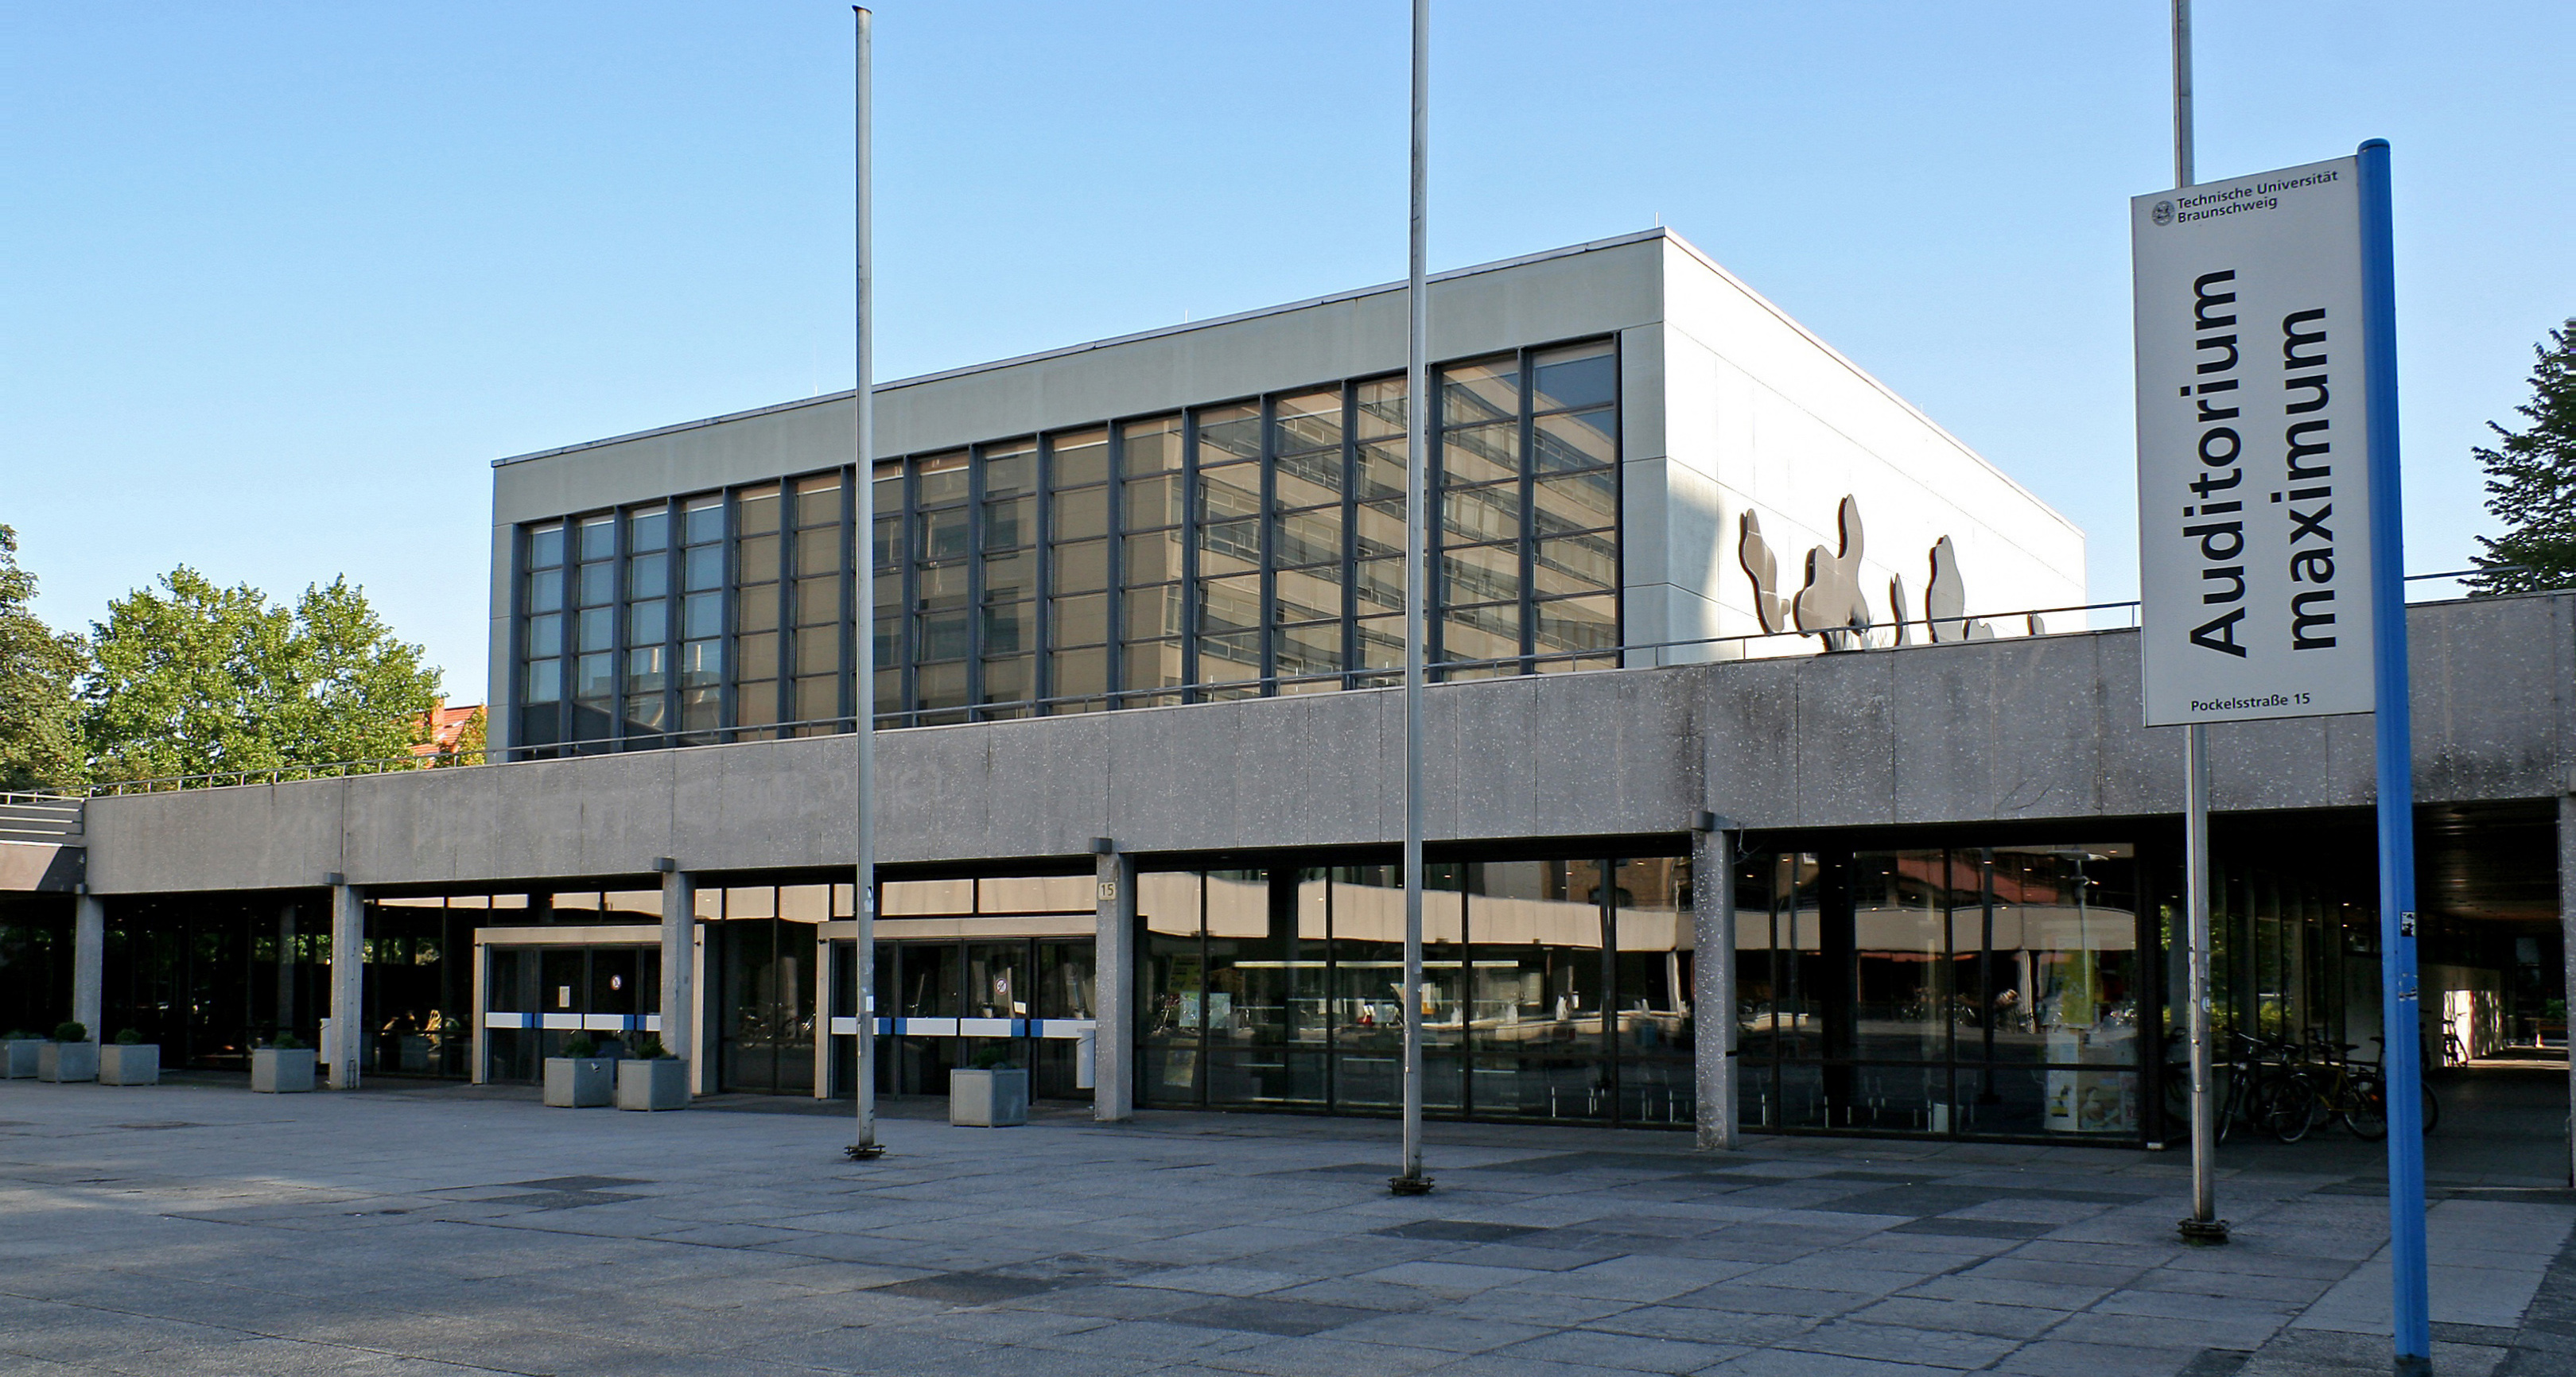
\includegraphics[width=\titlegraphicswidth]{titlepicture}}
\logo{
\includegraphics[height=\logoheight]{institut.jpg}}

\begin{document}

\begin{frame}[plain]
  \titlepage
\end{frame}

\begin{frame}{Inhaltsseite}
  \begin{itemize}
    \item Hier steht der Inhalt
    \item Hier nicht
    \item Weitere Informationen
  \end{itemize}
\end{frame}

\end{document}
\end{verbatim}

\begin{center}
  \fbox{\includegraphics[width=0.9\textwidth]{examples/titelseite.pdf}}

  \fbox{\includegraphics[width=0.9\textwidth]{examples/inhaltsseite.pdf}}
\end{center}
  % Kapitel: 'Präsentationen'


\chapter{Hintergrundlayout}

\begin{Declaration}
  \Macro{showtubslogo}\OParameter{Position}
\end{Declaration}

Bewirkt Darstellung des TU-Siegelbandlogos im aktiven Layout.
Die Option \PName{Position} erlaubt die Angabe der Darstellungsseite
(links/rechts). Standardmäßig wird das Logo links bzw. innen dargestellt.

\begin{Declaration}
  \Macro{showlogo}\PParameter{Logo}
\end{Declaration}

Bewirkt Darstellung eines Individuellen Logos im aktuellen Layout.
\PName{Logo} kann dabei entweder einfacher Text oder auch ein 
mit \Macro{includegraphics} eingebundenes Bild sein.

Die Positionierung wird automatisch an die Positionierung des Siegelbandlogos
angepasst. Wird dies links bzw. innen platziert, so steht das individuelle
Logo rechts bzw. außen.

\begin{Declaration}
  \Macro{showtopline}
\end{Declaration}

Bewirkt Darstellung einer Trennlinie zwischen Absender und Kommunikationsbereich
im aktuellen Layout.

\begin{Declaration}
  \Macro{bgelement}\OParameter{Darstellung}\PParameter{Höhe}
\end{Declaration}

Erstellt ein Hintergrundelement im Gaußraster mit angegebener \PName{Höhe}.
Der Parameter \PName{Darstellung} kann die folgenden Einstellungen verarbeiten:

\begin{Declaration}
  \KOption{bgcolor}\PName{Farbe}\\
  \KOption{bgimage}\PName{Bild-Datei}\\
  \KOption{imagefit}\PName{Darstellungsoption}
\end{Declaration}

Mit \OptionValue{bgcolor}{Farbe} wird das Hintergrundelement mit der angegebenen
Farbe gefüllt.

Die Option \OptionValue{bgimage}{Bild-Datei} erlaubt dagegen die Darstellung
eines Hintergrundbildes im Element.
Da der Darstellungsbereich fest vorgegeben ist, muss das eingebundene Bild
in diesen Bereich eingepasst werden. Dies geschieht automatisch, die Art
der Einpassung lässt sich aber mit der Option \Option{imagefit} kontrollieren.
Sie erlaubt folgende Einstellungen:


\begin{desctable}
\entry{\PValue{cropped}}{%
  Automatisches Abschneiden. Dies ist die Standardeinstellung.
}
\entry{\PValue{cropx}}{%
  Abschnitt horizontal.
}
\entry{\PValue{cropy}}{%
  Abschnitt vertikal.
}
\entry{\PValue{scaled}}{%
  Horizontale \emph{und} vertikale Skalierung.
}
\end{desctable}

\part{Basis-Pakete}

Dieser Abschnitt befasst sich mit den Paketen, die von den jeweiligen
\tubslatex-Anwenderklassen normalerweise automatisch geladen werden.
Diese Pakete stellen einige grundlegende Funktionalitäten und Darstellungen
für das \CD der TU Braunschweig dar. Dazu gehören zum einen das Paket
\newpackage{tubscolors}, das alle Farben, die im \CD vorgesehen sind,
definiert. Des weiteren gibt es das Paket \newpackage{tubslogo}, welches
zur Darstellung des Siegelbandlogos dient. Abschließend ist noch das Paket
\newpackage{nexus} zu erwähnen, welches die Hausschrift \emph{Nexus}
lädt.

All diese Pakete sind so konzipiert, dass sie auch unabhängig von den
Klassen und Paketen aus \tubslatex eingesetzt werden können, auch wenn dies
im Allgemeinen nicht erforderlich sein sollte.

\chapter{Farben}\label{sec:tubscolors}
\Index{Farben|indexbf}

\newcommand{\classoptionitem}[1][ ]{
  \item[\mdseries{\ttfamily%
    \textbackslash usepackage%
    {[{\color{tuRed}#1}]}%
    \{tubslogo\}}]\hfill\\
}

Die Farbdefinitionen in \tubslatex werden vom Paket \newpackage{tubscolors}
zur Verfügung gestellt. Die folgende Beschreibung bezieht sich
auf den Funktionsumfang dieses Paketes.
Da das Paket aber in allen verfügbaren \tubslatex-Klassen fest eingebunden ist,
gelten die Erklärungen auch allgemein.

\newcommand{\rainbow}[2][\relax]{{\noindent\sffamily\footnotesize%
\ifx#1\relax\colorlet{fglbg}{black}\else\colorlet{fglbg}{#1}\fi
\colorbox{#2100}{\hbox to 0.188\textwidth{%
  \color{fglbg}\vphantom{Fg}#2{}100\hfill}}% 
\colorbox{#280}{\hbox to 0.188\textwidth{%
  \color{fglbg}\vphantom{Fg}#2{}80\hfill}}% 
\colorbox{#260}{\hbox to 0.188\textwidth{\vphantom{Fg}#2{}60\hfill}}% 
\colorbox{#240}{\hbox to 0.188\textwidth{\vphantom{Fg}#2{}40\hfill}}% 
\colorbox{#220}{\hbox to 0.188\textwidth{\vphantom{Fg}#2{}20\hfill}}\\% 
}}

\section{Verfügbare Farben}

Der Farbklang der TU-Braunschweig ist in eine Primär- und einen
Sekundärfarbbereich aufgeteilt.

Die Primärfarben bilden dabei Rot, Schwarz und Weiß, sowie in
20-Prozent-Schritten abgestufte Grautöne. Die Primärfarben dienen
vor allem zur Auszeichnung von Hintergrund, Textfarbe und dem TU-Logo.
Zur individuellen Gestaltung von Dokumenten ist der Sekundärfarbbereich
vorgesehen.

Die Sekundärfarben setzen sich aus 12 weiteren aufeinander abgestimmten
Farben zusammen, die 
in 4 Farbklänge (Gelb-Orange, Grün, Blau und Violett) mit je 3 Basisfarben
aufgeteilt sind.
Alle Sekundärfarben können in 20-Prozent-Schritten aufgehellt werden.

\subsection{Benennungsschema}
\Index{Farben!Benennungsschema}

Alle Farben tragen das Präfix \texttt{tubs} vor Ihrem Namen.
Der eigentliche Farbname setzt sich zusammen aus dem Namen
des Sekundärfarbklangs
(\texttt{Orange}, \texttt{Blue}, \texttt{Green}, \texttt{Violet}) 
und einer Farbvariante
(\texttt{Light}, \texttt{Medium}, \texttt{Dark})
gefolgt von der Prozentzahl ihrer Helligkeitsstufe
(\texttt{20}, \texttt{40}, \texttt{60}, \texttt{80}, \texttt{100}).

Die Farben können sowoh in Präfix-Notation
(\Color{tubs\textsf{<Variante>}\textsf{<Klang>}80})
als auch in Suffix-Notation (\Color{tubs\textmd{<Klang>}\textmd{<Variante>}80})
angegeben werden.

\begin{example}
  Die helle Variante des Blau in 60\%iger Helligkeit kann also
  über den Namen \Color{tubsBlueLight60} als auch
  \Color{tubsLightBlue60} gewählt werden.
\end{example}

Vereinfachte Varianten der Benennung gibt es unter anderem für die 100\%-Varianten.
Hier kann die Prozentzahl weggelassen werden.
\begin{important}
Die Primärfarbe \Color{tubsRed} ist \emph{nicht} identisch mit \Color{tubsRed100}
aus dem gelb-orange-Sekundärfarbbereich.
In diesem speziellen Fall handelt es sich um verschiedene Farben.
\end{important}
Auch für die \texttt{Medium}-Varianten ist kein Präfix/Suffix notwendig.
\begin{example}
  Die Medium-Variante des Grün in 100\%iger Helligkeit kann vereinfacht
  mit \Color{tubsGreen} bezeichnet werden.
\end{example}

Die drei Primärfarben rot, schwarz und weiß sind unter den Namen
\Color{tubsRed}, \Color{tubsBlack} und \Color{tubsWhite} verfügbar.

Im Folgenden werden die zu Verfügung stehenden Farben aufgelistet.
Die Standardnamen über die die einzelnen Farben angesprochen werden können,
sind in den Beispielfeldern angegeben.

\subsection{Primärfarben}
\Index{Primärfarben}
\Index{Farben!Primär-}

{\sffamily\footnotesize%
\colorbox{tubsRed}{\hbox to 0.188\textwidth{%
  \vphantom{Fg}tubsRed\hfill}}%
\colorbox{tubsBlack}{\hbox to 0.188\textwidth{%
  \color{white}\vphantom{Fg}tubsBlack\hfill}}%
\fcolorbox{tubsBlack}{tuWhite}{\hbox to 0.188\textwidth{%
  \vphantom{Fg}tubsWhite\hfill}}\\%
}

\rainbow[tuWhite]{tubsGray}

Zur Vereinfachung sind noch die Farben \Color{tubsGray} und
\Color{tubsLightGrey} definiert, die den Farben \Color{tubsGray60} und
\Color{tubsGray20} entsprechen.

Alle Graytöne sind darüber hinaus auch in britischer Schreibweise nutzbar
(\Color{tubsGrey}).


\pagebreak
\subsection{Sekundärfarben}
\Index{Sekundärfarben}
\Index{Farben!Sekundär-}

  tubsOrange\ldots\\
  \colorshow{Orange}{Light}
  \colorshow{Orange}{Medium}
  \colorshow{Orange}{Dark}\\[-1ex]
  tubsBlue\ldots\\
  \colorshow{Blue}{Light}
  \colorshow{Blue}{Medium}
  \colorshow{Blue}{Dark}\\[-1ex]
  tubsGreen\ldots\\
  \colorshow{Green}{Light}
  \colorshow{Green}{Medium}
  \colorshow{Green}{Dark}\\[-1ex]
  tubsViolet\ldots\\
  \colorshow{Violet}{Light}
  \colorshow{Violet}{Medium}
  \colorshow{Violet}{Dark}
%   \caption{Im CD definierte Farben und deren Benennung (Auszug)}


% \begin{example}
% In folgendem Beispiel wurde \lstinline{blau} als Farbklang ausgewählt:
% 
% tubsSecondary\ldots\\
% \colorshow{Secondary}{Light}
% \colorshow{Secondary}{Medium}
% \colorshow{Secondary}{Dark}\\[-1ex]
% \end{example}

\subsection{Farbmodelle}
\Index{Farbmodelle}

Die Farben sind für 3 Farbmodelle (\acrshort{RGB}, RGB beamer-optimiert, \acrshort{CMYK}) definiert.
Das gewünschte Farmodell kann durch Klassen- bzw. Paketoptionen gewählt werden.
Die einzelnen Klassen haben bereits das jeweils passende Farbmodell voreingestellt.

Zusätzlich kann eine Monochrom-Variante gewählt werden, die die Farbe
\Color{tusbRed} automatisch als Schwarz darstellt.


\clearpage
\section{Verwendung/Farbwahl}
\sloppy

% TODO: hier ist noch etwas Bedarf...

Die TU-Farben können nach dem oben erläuterten Schema abgerufen und verwendet
werden wie jede andere Farbe auch.

\paragraph{Haupt-Sekundärfarbklang}\label{sec:secondary}

Die Farben des aktuell gewählten Haupt-Sekundärfarbklangs können zusätzlich
über die Namen \Color{tuSecondaryLight},
\Color{tuSecondaryMedium}, \Color{tuSecondaryDark}, sowie die
entsprechenden Prozentualwert \Color{tuSecondaryLight20},
\Color{tuSecondaryLight40}, \ldots) angesprochen werden können.
Dies erlaubt eine flexible Verwendung der 4 Sekundärfarbklänge.

Die Wahl der Haupt-Sekundärfarbklangs erfolgt entweder über die weiter
unten beschriebenen Klassen-/Paketoptionen oder innerhalb des Dokumentes auch
mit dem Befehl \Macro{selectsecondary}.

\paragraph{Fettes Schwarz}\label{sec:richblack}
\Index{rich black|indexbf}
\Index{Schwarz!fettes|indexbf}

Bei der Verwendung des CMYK-Farbraums ist zu beachten,
dass das die Farbe Schwarz (\Color{tubsBlack})
der Mischung 0\%C, 0\%M, 0\%Y, 100\%K entspricht,
was in der Bildschirmdarstellung meist nur als sehr dunkles grau wahrgenommen wird.
Dies gilt somit auch für den Text im Dokument und ist normal.
Für Bildschirmdarstellung wird immer das RGB-Farbprofil empfohlen.

\begin{figure}[!ht]
\centering
{\selectcolormodel{cmyk}
\colorbox[cmyk]{0,0,0,1}{\parbox[t][2cm]{3cm}{\vfill\centering\sffamily\color{tubsWhite} tubsBlack\vfill}}%
\qquad
\colorbox[cmyk]{0.75,0.68,0.67,0.9}{\parbox[t][2cm]{3cm}{\vfill\centering\sffamily\color{tubsWhite} tubsRichBlack\vfill}}%
}
\caption{Vergleich der Farben \Color{tubsBlack} und \Color{tubsRichBlack} im CMYK-Farbraum}
\end{figure}


Im CMYK-Druck dagegen wird es mit der Key-Patrone gedruckt und daher korrekt
als Schwarz ausgegeben.
Sollte trotz dessen die Ausgabe aus dem Drucker zu hell erscheinen,
so kann dies entweder durch Verwendung der Klassen-/Paketoption \Option{richblack}
(siehe folgendes Kapitel) oder durch einen manuelle Anpassung der Farbe
\Color{tubsBlack} korrigiert werden, indem ein sogenanntes
\emph{Fettes Schwarz} (rich black) verwendet wird.
Dabei werden zusätzlich die CMY-Farben benutzt, um ein möglichst dunkles
Schwarz zu mischen. Die Standarddefinition der Option \Option{richblack}
entspricht dies  einer Mischung von 75\%C, 68\%M, 67\%Y, 90\%K.
Alternativ kann auch die definierte Farbe \Color{tubsRichBlack} verwendet werden.

Zu beachten ist jedoch, dass diese Farbe im Druck ggf. zu unsaubereren
Ergebnissen durch den übermäßigen Tinteneinsatz führen kann!
  
\begin{example}
  Manuelle Umdefinierung von \Color{tubsBlack}:\\
  \lstinline!\definecolor{tubsBlack}{CMYK}{0.5,0.5,0.5,1.0}!
\end{example}


\subsection{Paket-/Klassenoptionen und Befehle}
\Index{RGB}
\Index{RGB!Beamer}
\Index{CMYK}
\Index{monochrom}

\begin{Declaration}
  \Option{rgb}\\
  \Option{rgbbeamer}\\
  \Option{cmyk}\\[1ex]
  \Option{mono}
\end{Declaration}

Die Option \Option{rgb} bewirkt eine Darstellung der Farben im vordefinierten
RGB-Farbprofil.
Die Option \Option{rgbbeamer} lädt ein Beamer-optimierts RGB-Farbprofil.
Mit der Option \Option{cmyk} wird das CMYK-Farbprofil geladen.
Die Zusatz-Option \Option{mono} bewirkt eine Darstellung der Farbe
\Color{tubsRed} als \Color{tubsBlack} im aktuell gewählten Farbprofil.
Dies kann insbesondere für schwarz-weiß Kopiervorlagen in Verbindung
mit der schwarzen Siegelbandlogo-Variante sinnvoll sein.


\begin{Declaration}
  \Option{richblack}
\end{Declaration}

Definiert die Farbe \Color{tubsBlack} bei Verwendung des CMYK-Farbprofils
in ein sog. "`fettes Schwarz"' um. Siehe dazu auch Abschnitt~\ref{sec:richblack}.

\begin{Declaration}
  \Option{orange}\\
  \Option{green}\\
  \Option{blue}\\
  \Option{violet}
\end{Declaration}

Mit diesen Optionen kann der Standard-Sekundärfarbklang des Dokumentes gewählt
werden. Der jeweils geladene Sekundärfarbklang ergibt sich aus dem Namen
der Option.
Die Farben des Sekundärfarbklangs können wie in Abschnitt~\ref{sec:secondary}
beschrieben benutzt werden.

\begin{Declaration}
  \Macro{selectsecondary}\Parameter{Farbklang}
\end{Declaration}

Befehl zur Wahl des Haupt-Sekundärfarbklangs. Als Option für \PName{Farbklang}
sind die Werte \PValue{orange}, \PValue{green}, \PValue{blue} und \PValue{violet}
erlaubt.

\begin{Declaration}
  \Macro{tubscolorshow}\Parameter{Farbe}\Parameter{Variante}
\end{Declaration}

Zeigt farbige Boxen mit allen Helligkeitsstufen der angegebenen Farbklang-Variante.
\begin{example}
 Die Ausgabe von \lstinline!\tubscolorshow{Blue}{Light}! sieht beispielsweise
 wie folgt aus:\\
 \hspace*{-1cm}\tubscolorshow{Blue}{Light}
\end{example}

\fussy
  % Kapitel: 'Farben'

\chapter{Das Siegelbandlogo}

Die verschiedenen Farbvarianten des Siegelbandlogos in \tubslatex werden
vom Paket \lstinline{tubslogo} zur Verfügung gestellt.
Die folgende Beschreibung bezieht sich auf den Funktionsumfang des Paketes.
Das Paket ist in allen verfügbaren Klassen bereits korrekt eingebunden.

Zur Verfügung gestellt werden eine Variante im rgb-Farbmodell, eine im
cmyk-Farbmodell, eine mit der Sonderfarbe HKS 15 oder (für Ausnahmefälle)
eine monochromen Variante.
Die Auwahl erfolgt dabei über Paketoptionen
(siehe Abschnitt \ref{options:color}).

\begin{figure}[!ht]
\begin{minipage}{0.5\textwidth}
  \centering
  
\includegraphics[width=\tubslogoBaseWidth]{TUBraunschweig_RGB}
  \subcaption{Logo in Standardgröße (RGB)}
\end{minipage}
\begin{minipage}{0.5\textwidth}
  \centering
  
\includegraphics[width=\tubslogoBaseWidth]{TUBraunschweig_4C}
  \subcaption{Logo in Standardgröße (CMYK)}
\end{minipage}

\begin{minipage}{0.5\textwidth}
  \centering
  
\includegraphics[width=\tubslogoBaseWidth]{TUBraunschweig_SC}
  \subcaption{Logo in Standardgröße (HKS 15)}
\end{minipage}
\begin{minipage}{0.5\textwidth}
  \centering
  
\includegraphics[width=\tubslogoBaseWidth]{TUBraunschweig_B}
  \subcaption{Logo in Standardgröße (schwarz)}
\end{minipage}
\caption{Verfügbare Farbversionen der Logos}
\end{figure}

\begin{Declaration}
  \Macro{tubslogo}\OParameter{Skalierung}\\
  \Macro{tubslogoAbs}\Parameter{Breite}
\end{Declaration}


Es werden 2 Befehle zum Einfügen des Logos in Dokumente bereit gestellt.
Mit dem Befehl \Macro{tubslogo} wird ein Logo in
standardkonformer Größe der verwendeten Papiergröße entsprechend skaliert
eingefügt. Die verwendete Papiergröße kann dabei als Paketoption übergeben
werden und ist standardmäßig auf \lstinline{a4paper} voreingestellt
(siehe Abschnitt \ref{options:papersize}).
Als optionales Argument kann auch ein frei gewählter Skalierungsfaktor
vorgegeben werden (siehe Abschnitt \ref{cmd:tubslogo}).

Mit \Macro{tubslogoAbs} kann über den Parameter \PName{Breite} dagegen
zusätzlich eine individuell gewählte absolute Breite angegeben werden.


\section{Paket-Optionen}

\subsection{Farbmodell}\label{options:color}

\begin{description}
  \classoptionitem[rgb]
    Verwendung der rgb-Druckfarben. Dies ist die Standardeinstellung.
  \classoptionitem[cmyk]
    Verwendung der cmyk-Farben
  \classoptionitem[hks]
    Verwendung der Spezialfarbe HKS 15.
  \classoptionitem[mono]
    Verwendung einer schwarz-weiß-Version des Logos.
\end{description}

\subsection{Papiergröße}\label{options:papersize}

\begin{description}
  \classoptionitem[a6paper]
    Skaliert das Logo passend für A6-Dokumente auf 60\% der Standardgröße.
  \classoptionitem[a5paper]
    Skaliert das Logo passend für A5-Dokumente auf 70\% der Standardgröße.
  \classoptionitem[a4paper]
    Skaliert das Logo passend für A4-Dokumente auf Standardgröße.
  \classoptionitem[a3paper]
    Skaliert das Logo passend für A3-Dokumente auf 140\% der Standardgröße.
  \classoptionitem[a2paper]
    Skaliert das Logo passend für A2-Dokumente auf 200\% der Standardgröße.
  \classoptionitem[a1paper]
    Skaliert das Logo passend für A1-Dokumente auf 280\% der Standardgröße.
  \classoptionitem[a0paper]
    Skaliert das Logo passend für A0-Dokumente auf 400\% der Standardgröße.
\end{description}


\clearpage
\section{Befehle}

\begin{description}\label{cmd:tubslogo}
  \item[\color{tuRed}\mdseries\ttfamily \textbackslash tubslogo%
    {[\textcolor{tuGreenDark}{\sffamily\itshape $<$Breite rel.$>$}]}]
    Erzeugt ein Logo, dass entsprechend des durch Angabe der Papiergröße
    gewählten Skalierungsfaktors skaliert wird.

    Wird das optionale Argument {\sffamily\itshape $<$Breite rel.$>$}
    verwendet, so kann ein freier Skalierungsfaktor ausgehend von der
    Standardgröße für DINA4-Dokumente ($70$mm$\times 26$mm) übergeben werden.

    \lstinline!\tubslogo[0.6]! erzeugt beispielsweise ein auf 60\% der 
    Standardgröße für DINA4-Dokumente skaliertes Logo.

  \item[\color{tuRed}\mdseries\ttfamily \textbackslash tubslogoAbs%
    \{\textcolor{tuGreenDark}{Breite abs.}\}]
    Dieser Befehl erlaubt die Erzeugung eines Logos mit absolut vorgegebener
    Breite.\footnote{Generell ist die Verwendung von standardkonformen Größen
    einer individuellen Skalierung vorzuziehen!}

    \lstinline!\tubslogoAbs{5cm}! erzeugt beispielsweise ein 5cm breites Logo.
\end{description}


\section{Längen}
  \begin{description}
    \item[\mdseries\ttfamily \textbackslash tubslogoBaseWidth]\hfill\\
      Standardbreite des Logos (70mm).
    \item[\mdseries\ttfamily \textbackslash tubslogoBaseHeight]\hfill\\
      Standardhöhe des Logos (26mm).
    \item[\mdseries\ttfamily \textbackslash tubslogoWidth]\hfill\\
      Breite des automatisch skalierten Logos. Wird automatisch berechnet und
      kann zur dynamischen Positionierung verwendet werden.
    \item[\mdseries\ttfamily \textbackslash tubslogoHeight]\hfill\\
      Höhe des automatisch skalierten Logos. Siehe \lstinline{tubslogoWidth}.
  \end{description}
    % Kapitel: 'Logo'

% \iffalse meta-comment
%
% Copyright (C) 2011 by Enrico Jörns
% -----------------------------------
%
% This file may be distributed and/or modified under the
% conditions of the LaTeX Project Public License, either version 1.2
% of this license or (at your option) any later version.
% The latest version of this license is in:
%
%   http://www.latex-project.org/lppl.txt
%
% and version 1.2 or later is part of all distributions of LaTeX
% version 1999/12/01 or later.
%
% \fi
%
% \CheckSum{0}
%
% \CharacterTable
%  {Upper-case    \A\B\C\D\E\F\G\H\I\J\K\L\M\N\O\P\Q\R\S\T\U\V\W\X\Y\Z
%   Lower-case    \a\b\c\d\e\f\g\h\i\j\k\l\m\n\o\p\q\r\s\t\u\v\w\x\y\z
%   Digits        \0\1\2\3\4\5\6\7\8\9
%   Exclamation   \!     Double quote  \"     Hash (number) \#
%   Dollar        \$     Percent       \%     Ampersand     \&
%   Acute accent  \'     Left paren    \(     Right paren   \)
%   Asterisk      \*     Plus          \+     Comma         \,
%   Minus         \-     Point         \.     Solidus       \/
%   Colon         \:     Semicolon     \;     Less than     \<
%   Equals        \=     Greater than  \>     Question mark \?
%   Commercial at \@     Left bracket  \[     Backslash     \\
%   Right bracket \]     Circumflex    \^     Underscore    \_
%   Grave accent  \`     Left brace    \{     Vertical bar  \|
%   Right brace   \}     Tilde         \~}
%
% \iffalse
%
%<*driver>
\documentclass{tubsltxdoc}
\usepackage[ngerman]{babel}
\usepackage[utf8]{inputenc}
\usepackage{nexus}
\usepackage[colorlinks, linkcolor=blue]{hyperref}
\usepackage{tabularx}
\EnableCrossrefs
\CodelineIndex
\RecordChanges
\begin{document}
  \DocInput{nexus.dtx}
\end{document}
%</driver>
% \fi
%
%
% \changes{v0.2}{ 2011 / 08 / 23 }{%
%   Initial version}
% \changes{v0.3}{ 2011 / 10 / 13 }{%
%   Optionen 'nexus' und 'arial' hinzugefügt,
%   mathpazo als Standard-Mathe-Font.}
% \changes{v0.4}{ 2011 / 10 / 26 }{%
%   Option 'arial' aktiviert nun automatisch sffamily}
%
% \GetFileInfo{nexus.sty}
%
% \DoNotIndex{ list of control sequences }
%
% \title{\textsf{nexus} -- 
%   CD-Schrift für \emph{tubslatex}\thanks{This document
%   corresponds to \textsf{nexus}~\fileversion,
%   dated \filedate.}}
% \author{Enrico Jörns \\ \texttt{e dot joerns at tu minus bs dot de}}
%
% \maketitle
%
% \begin{abstract}
%   Diese Datei stellt die Schriftart \emph{Nexus} zur Verfügung.
% \end{abstract}
%
% \StopEventually{\PrintIndex}
%
% \section{Schriftübersicht}
%
% \subsection{Serif}
% 
% \paragraph{Normal}\hfill\\
% {
% Lorem ipsum dolor sit amet, consectetur adipisici elit, sed eiusmod tempor
% incidunt ut labore et dolore magna aliqua.}
% \paragraph{Italic}\hfill\\
% {\itshape
% Lorem ipsum dolor sit amet, consectetur adipisici elit, sed eiusmod tempor
% incidunt ut labore et dolore magna aliqua.}
% \paragraph{Slanted}\hfill\\
% {\slshape
% Lorem ipsum dolor sit amet, consectetur adipisici elit, sed eiusmod tempor
% incidunt ut labore et dolore magna aliqua.}
% \paragraph{SmallCaps}\hfill\\
% {\scshape
% Lorem ipsum dolor sit amet, consectetur adipisici elit, sed eiusmod tempor
% incidunt ut labore et dolore magna aliqua.}
% 
% {\bfseries
% \paragraph{Bold Normal}\hfill\\
% {
% Lorem ipsum dolor sit amet, consectetur adipisici elit, sed eiusmod tempor
% incidunt ut labore et dolore magna aliqua.}
% \paragraph{Bold Italic}\hfill\\
% {\itshape
% Lorem ipsum dolor sit amet, consectetur adipisici elit, sed eiusmod tempor
% incidunt ut labore et dolore magna aliqua.}
% \paragraph{Bold Slanted}\hfill\\
% {\slshape
% Lorem ipsum dolor sit amet, consectetur adipisici elit, sed eiusmod tempor
% incidunt ut labore et dolore magna aliqua.}
% \paragraph{Bold SmallCaps}\hfill\\
% {\scshape
% Lorem ipsum dolor sit amet, consectetur adipisici elit, sed eiusmod tempor
% incidunt ut labore et dolore magna aliqua.}
% }
% 
% \subsection{SansSerif}
% 
% {\sffamily
% \paragraph{Normal}\hfill\\
% {
% Lorem ipsum dolor sit amet, consectetur adipisici elit, sed eiusmod tempor
% incidunt ut labore et dolore magna aliqua.}
% \paragraph{Italic}\hfill\\
% {\itshape
% Lorem ipsum dolor sit amet, consectetur adipisici elit, sed eiusmod tempor
% incidunt ut labore et dolore magna aliqua.}
% \paragraph{Slanted}\hfill\\
% {\slshape
% Lorem ipsum dolor sit amet, consectetur adipisici elit, sed eiusmod tempor
% incidunt ut labore et dolore magna aliqua.}
% \paragraph{SmallCaps}\hfill\\
% {\scshape
% Lorem ipsum dolor sit amet, consectetur adipisici elit, sed eiusmod tempor
% incidunt ut labore et dolore magna aliqua.}
% 
% {\bfseries
% \paragraph{Bold Normal}\hfill\\
% {
% Lorem ipsum dolor sit amet, consectetur adipisici elit, sed eiusmod tempor
% incidunt ut labore et dolore magna aliqua.}
% \paragraph{Bold Italic}\hfill\\
% {\itshape
% Lorem ipsum dolor sit amet, consectetur adipisici elit, sed eiusmod tempor
% incidunt ut labore et dolore magna aliqua.}
% \paragraph{Bold Slanted}\hfill\\
% {\slshape
% Lorem ipsum dolor sit amet, consectetur adipisici elit, sed eiusmod tempor
% incidunt ut labore et dolore magna aliqua.}
% \paragraph{Bold SmallCaps}\hfill\\
% {\scshape
% Lorem ipsum dolor sit amet, consectetur adipisici elit, sed eiusmod tempor
% incidunt ut labore et dolore magna aliqua.}
% }
% }
% 
%
% \subsection{Nexus Symbol-Tabelle {\normalsize\mdseries (auszugsweise)}}
% {
% \parindent0mm
% 
% 1, 2, 3, 4, 5, 6, 7, 8, 9, 0
% 
% a, b, c, d, e, f, g, h, i, j, k, l, m, n, o, p, q, r, s, t, u, v, w, x, y, z
% 
% A, B, C, D, E, F, G, H, I, J, K, L, M, N, O, P, Q, R, S, T, U, V, W, X, Y, Z
% 
% ä, ö, ü, ß, Ä, Ö, Ü
% 
% *, +, -, =, \textasciitilde, \textasciicircum, , !, ", §, \$, \%, \&,
% /, (, ), =, ?, µ, @,\{, \}, [, ]
% }
%
%
% \subsection{Typewriter- / Mathe-Font}
% 
% Der Typewriter-Font stammt nicht aus Nexus, sondern wird aus dem
% \emph{TxFonts}-Satz übernommen.
% 
% Als Mathe-Font dient die \emph{Pazo Math}-Familie.
%
% \section{Implementierung}
%
%
%    \begin{macrocode}
%<*package>
%    \end{macrocode}
%
%    \begin{macrocode}
\ProvidesPackage{nexus} [2011/10/26 v0.4 Nexus support for LaTeX]
%    \end{macrocode}
%
%    \begin{macrocode}
\RequirePackage{xkeyval}
\newif\ifnexus@usearial\nexus@usearialfalse
%    \end{macrocode}
%
%    \begin{key}{}{arial}
%    \begin{macrocode}
\DeclareOptionX{arial}{%
  \nexus@usearialtrue
}
%    \end{macrocode}
%    \end{key}
%
%    \begin{key}{}{nexus}
%    \begin{macrocode}
\DeclareOptionX{nexus}{%
  \nexus@usearialfalse
}
%    \end{macrocode}
%    \end{key}
%
%    \begin{key}{}{lnum}
% Verwende Versalziffern (lining figures) anstellen von Mediävalziffern.
% Funktioniert nur bei Nexus!
%    \begin{macrocode}
\newif\ifnexus@lnum\nexus@lnumfalse
\DeclareOptionX{lnum}{%
  \nexus@lnumtrue
}
%    \end{macrocode}
%    \end{key}
%
% Behandle Optionen
%    \begin{macrocode}
\ProcessOptionsX*\relax
%    \end{macrocode}
%
% Testen, ob Option 'arial' gewählt wurde.\par
% Behandlung für Option 'arial'
%    \begin{macrocode}
\ifnexus@usearial%
%    \end{macrocode}
%
% Arial und passende Pakete laden
%    \begin{macrocode}
\RequirePackage[scaled]{uarial} % for T1 encoding
\RequirePackage[OT1]{eulervm}% don't know why OT1 is required here, but it is.
\PassOptionsToPackage{T1}{fontenc}
\renewcommand*{\encodingdefault}{T1}
\RequirePackage{fontenc}
\renewcommand{\familydefault}{\sfdefault}
%    \end{macrocode}
%
% Support für babels latintext (used by LaTeX, TeX, etc.)
%    \begin{macrocode}
\AtBeginDocument{%
\ifx\@undefined\latintext%
\else%
\renewcommand{\latintext}{%
\ifx\f@family\rmdefault%
\fontencoding{\latinencoding}\fontfamily{ptm}\selectfont%
\else%
  \ifx\f@family\sfdefault%
  \fontencoding{\latinencoding}\fontfamily{ua1}\selectfont%
  \else%
  \fi%
\fi%
\def\encodingdefault{\latinencoding}}%
\fi%
}
%    \end{macrocode}
%
%    \begin{macrocode}
\let\lnum\relax
%    \end{macrocode}
%
% Behandlung für Option 'nexus'
%    \begin{macrocode}
\else% -> \ifnexus@usearial
%    \end{macrocode}
%
% Lade benötigte Pakete
%    \begin{macrocode}
\RequirePackage{mathpazo}
\PassOptionsToPackage{LY1}{fontenc}
\RequirePackage{fontenc}
%    \end{macrocode}
%
% 
%    \begin{macro}{\glq}
%    \begin{macro}{\grq}
% Anführungszeichen deutsch -- einfach
%    \begin{macrocode}
\ProvideTextCommand{\glq}{LY1}{\symbol{0130}}
\ProvideTextCommand{\grq}{LY1}{\symbol{0096}}
%    \end{macrocode}    
%    \end{macro}\end{macro}
%
%    \begin{macro}{\glqq}
%    \begin{macro}{\grqq}
% Anführungszeichen deutsch -- doppelt
%    \begin{macrocode}
\ProvideTextCommand{\glqq}{LY1}{\symbol{0132}}
\ProvideTextCommand{\grqq}{LY1}{\symbol{0147}}
%    \end{macrocode}    
%    \end{macro}\end{macro}
%
%    \begin{macro}{\flq}
%    \begin{macro}{\flq}
% Anführungszeichen französisch -- einfach
%    \begin{macrocode}
\ProvideTextCommand{\flq}{LY1}{\symbol{0139}}
\ProvideTextCommand{\frq}{LY1}{\symbol{0155}}
%    \end{macrocode}    
%    \end{macro}\end{macro}
%
%    \begin{macro}{\flqq}
%    \begin{macro}{\frqq}
% Anführungszeichen französisch -- doppelt
%    \begin{macrocode}
\ProvideTextCommand{\flqq}{LY1}{\symbol{0171}}
\ProvideTextCommand{\frqq}{LY1}{\symbol{0187}}
%    \end{macrocode}    
%    \end{macro}\end{macro}
%
%    \begin{macro}{\textasteriskcentered}
%    \begin{macrocode}
\DeclareTextCommand{\textasteriskcentered}{LY1}{$*$}
%    \end{macrocode}
%    \end{macro}
%
% Nexus verwenden.
%    \begin{macrocode}
\renewcommand*{\encodingdefault}{LY1}
\ifnexus@lnum
  \renewcommand*{\rmdefault}{NexusProSerif-lnum}
  \renewcommand*{\sfdefault}{NexusProSans-lnum}
\else
  \renewcommand*{\rmdefault}{NexusProSerif}
  \renewcommand*{\sfdefault}{NexusProSans}
\fi
\renewcommand*{\ttdefault}{txtt} % with bold series!
%    \end{macrocode}
%
%    \begin{macro}{\lnum}
% Schaltet auf Versalziffern (newstyle/lining numbers) um.
%    \begin{macrocode}
\newcommand\lnum{%
  \def\@test{NexusProSerif}%
  \ifx\f@family\@test%
    \fontfamily{NexusProSerif-lnum}%
  \else
    \fontfamily{NexusProSans-lnum}%
  \fi
  \selectfont
}
%    \end{macrocode}
%    \end{macro}

%    \begin{macro}{\textlnum}
% Setzt Text mit Versalziffern
%    \begin{macrocode}
\newcommand\textlnum[1]{%
  {\lnum #1}%
}
%    \end{macrocode}
%    \end{macro}
%
%    \begin{macro}{\oldstylenums}
% Schaltet auf Mediävalziffern (oldstyle/text numbers) um.
%    \begin{macrocode}
\newcommand\onum{%
  \def\@test{NexusProSerif-lnum}%
  \ifx\f@family\@test%
    \fontfamily{NexusProSerif}%
  \else
    \fontfamily{NexusProSans}%
  \fi
  \selectfont
}

%    \end{macrocode}
%    \end{macro}
%
%    \begin{macro}{\oldstylenums}
% Setzt Text mit Mediävalziffern
%    \begin{macrocode}
\renewcommand{\oldstylenums}[1]{%
  {\onum #1}%
}
%    \end{macrocode}
%    \end{macro}
%
% mathsf und mathtt passend definieren
%    \begin{macrocode}
\SetMathAlphabet{\mathsf}{normal}{LY1}{NexusProSans}{m}{n}
\SetMathAlphabet{\mathtt}{normal}{LY1}{txtt}{m}{n}
%    \end{macrocode}
%
% Support für babels latintext (used by LaTeX, TeX, etc.)
%    \begin{macrocode}
\AtBeginDocument{%
\ifx\@undefined\latintext%
\else%
\renewcommand{\latintext}{%
\ifx\f@family\rmdefault%
\fontencoding{LY1}\fontfamily{NexusProSerif}\selectfont%
\else%
  \ifx\f@family\sfdefault%
  \fontencoding{LY1}\fontfamily{NexusProSans}\selectfont%
  \else%
  \fi%
\fi%
\def\encodingdefault{LY1}}%
\fi%
}
%    \end{macrocode}
%
%    \begin{macro}{\LaTeX}
% Korrigierte Abstände für Logo unter Nexus
%    \begin{macrocode}
% TODO: fix capacity error
% \def\LaTeX{L\kern-.32em\raise.3ex\hbox{\scalebox{0.76}{A}}\kern-.15em\TeX}%
%    \end{macrocode}
%    \end{macro}
%
%    \begin{macrocode}
\fi%
%    \end{macrocode}
%
%    \begin{macrocode}
%</package>
%    \end{macrocode}
%
% \Finale
\endinput
%
   % Kapitel: 'Nexus'


%Befehle für Glossar
\newglossaryentry{glos:siegelbandlogo}{%
  name=Siegelbandlogo,
  description={\tubslogo}
}
\newglossaryentry{glos:gaussraster}{%
  name={Gau\ss raster},
  description={Auf der gaußschen Summenformel basierende Unterteilung der Seite
    in Segmente. Benachbarte Segmente können beliebig zusammen gefasst werden}
}
\newglossaryentry{glos:cmyk}{%
  name={CMYK-Farbmodell},
  description={Das CMYK-Farbmodell ist ein subtraktives Farbmodell,
    das die technische Grundlage für den modernen Vierfarbdruck bildet.
    Die Abkürzung CMYK steht für die drei Farbbestandteile
    \emph{Cyan}, \emph{Magenta}, \emph{Yellow}
    und den Schwarzanteil \emph{Key} als Farbtiefe}
}
\newglossaryentry{glos:absenderbereich}{%
  name={Absenderbereich},
  description={Bereich zur Darstellung von Absendern}
}
\newglossaryentry{glos:kommunikationsbereich}{%
  name={Absenderbereich},
  description={Bereich zur Darstellung von Inhalten}
}
\newglossaryentry{glos:spaltenraster}{%
  name={Spaltenraster},
  description={Abhängig vom Format kann der Textbereich einer Seite in
    6, 4 oder 2 Grundspalten geteilt werden, welche alle die selbe Breite und
    den selben Abstand zueinander haben.
    Benachbarte Grundspalten können variabel zu einer Darstellungsspalte
    zusammengefasst werden}
}
\newglossaryentry{glos:bindekorrektur}{%
  name={Bindekorrektur},
  description={}
}
\newglossaryentry{glos:sekundaerfarbklang}{%
  name={Sekund\"arfarbklang},
  description={}
}

%Akronyme
\newacronym{CD}{CD}{Corporate Design}
\newacronym{CMYK}{CMYK}{Cyan, Magenta, Yellow, Key}


\appendix

\chapter{lco-Dateien}
\section{Institut}
\lstinputlisting{../../letter/doc/examples/musterinstitut.lco}
\section{Mitarbeiter}
\lstinputlisting{../../letter/doc/examples/mustermann.lco}


\bibliographystyle{alpha}
\bibliography{lit}

\end{document}
